\documentclass[12pt]{beamer}


\usetheme[progressbar=frametitle]{metropolis}
\usepackage{appendixnumberbeamer}

\usepackage{booktabs}
\usepackage[scale=2]{ccicons}

%\usepackage{pgfplots}
%\usepgfplotslibrary{dateplot}

\usepackage{xspace}
\newcommand{\themename}{\textbf{\textsc{metropolis}}\xspace}

%\setbeamertemplate{footline} % To remove the footer line in all slides uncomment this line
%\setbeamertemplate{footline}[page number] % To replace the footer line in all slides with a simple slide count uncomment this line

%\setbeamertemplate{navigation symbols}{} % To remove the navigation symbols from the bottom of all slides uncomment this line


\usepackage{graphicx} % Allows including images
\usepackage{grffile}
\usepackage{amsmath}
\usepackage{adjustbox} 
% have to have Mozilla's=Fira Sans} font and XeTeX installed to use full typography.

%----------------------------------------------------------------------------------------
%	TITLE PAGE
%----------------------------------------------------------------------------------------

\title{Alliance Participation, Treaty Depth, and Military Spending}
\date{August 26, 2020}
\author{Joshua Alley}
\institute{University of Virginia}


\begin{document}

 \maketitle


%----------------------------------------------------------------------------------------
%	PRESENTATION SLIDES
%----------------------------------------------------------------------------------------

%------------------------------------------------
% Here's my point. 
 \begin{frame}[standout]

How does alliance participation affect military spending?  

 \end{frame}
 

%%------------------------------------------------
% 
% \begin{frame}{A Tale of Two Franco-Belgian Alliances} 
%
%\begin{columns}
%
%\uncover<2->{
%\begin{column}{0.5\textwidth}
%\textbf{France and Belgium 1920}
%
%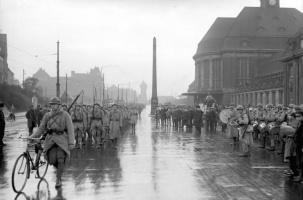
\includegraphics[width = .95\textwidth]{franco-belgian-rhineland.jpg} 
%
%\end{column}
%}
%
%
%\uncover<3->{
%\begin{column}{0.5\textwidth}
%\textbf{France, Belgium and Company 1925}
% 
%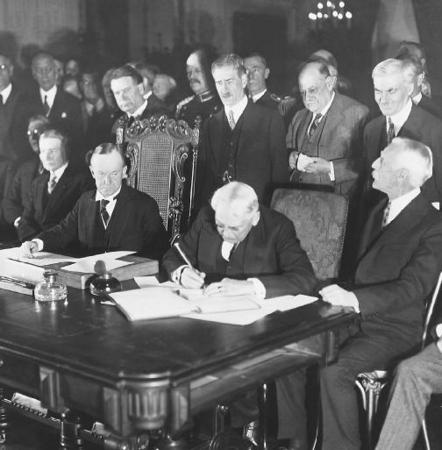
\includegraphics[width = .95\textwidth]{locarno-sign.jpeg}  
% 
%\end{column}
%}
%
%\end{columns}
%
% \end{frame}
 
 
%------------------------------------------------

\begin{frame}{Competing Claims and Results}

\begin{table}[hbt!]
\begin{center}
  \resizebox{.95\textheight}{!}{
\begin{tabular}{lccc}
     & Decrease & Increase & Null \\
\hline
Most \& Siverson 1987  &  &  & X \\
Conybeare 1994 & X & &  \\
Diehl 1994 &  & X &  \\
Goldsmith 2003 &  &  & X \\
Morgan \& Palmer 2006 &  & X & \\ 
Quiroz-Flores 2011 &  & X &  \\
Conybeare \& Sandler 1990 &   & X &  \\
Barnett \& Levy 1991 & X  &  &  \\
Morrow 1993  & X  &  &  \\
Sorokin 1994 & X  &  &  \\
Chen et al 1996 &    & X &  \\
Pluemper \& Neumayer 2015 & X &  &  \\
George \& Sandler 2017 & X &  &  \\ 
\hline
\end{tabular}
}
\end{center} 
\end{table}


\end{frame}
 

%------------------------------------------------

\begin{frame}[standout]

\huge \textit{Does alliance participation increase military spending?} \uncover<2->{Or decrease it?}

\end{frame}

%------------------------------------------------

\begin{frame}{Alliance Heterogeneity}


\begin{itemize}
\item Alliances can \textit{increase or decrease} military spending. 
\pause
\item Depends on alliance characteristics and states' foreign policy goals.  
\pause 
\item \textbf{Treaty depth is a key source of differences between alliances.}
\end{itemize} 

\end{frame}


%------------------------------------------------
% Here's my point. 
 \begin{frame}[standout]

Deep alliances often decrease non-major power military spending, but shallow alliances often increase it.   

 \end{frame}
 
 
 %------------------------------------------------
% Here's my point. 
 \begin{frame}{What Does That Mean?} 

\begin{itemize}
\item \textbf{Depth}: The extent of military cooperation an alliance treaty promises.
\pause 
\item \textbf{Non-major powers}: Countries with less capability and ambition in international politics. 
\end{itemize}

 \end{frame}
 
 
 
%------------------------------------------------

\begin{frame}{Why Should You Care?}

\begin{figure}[htbp]
	\centering
		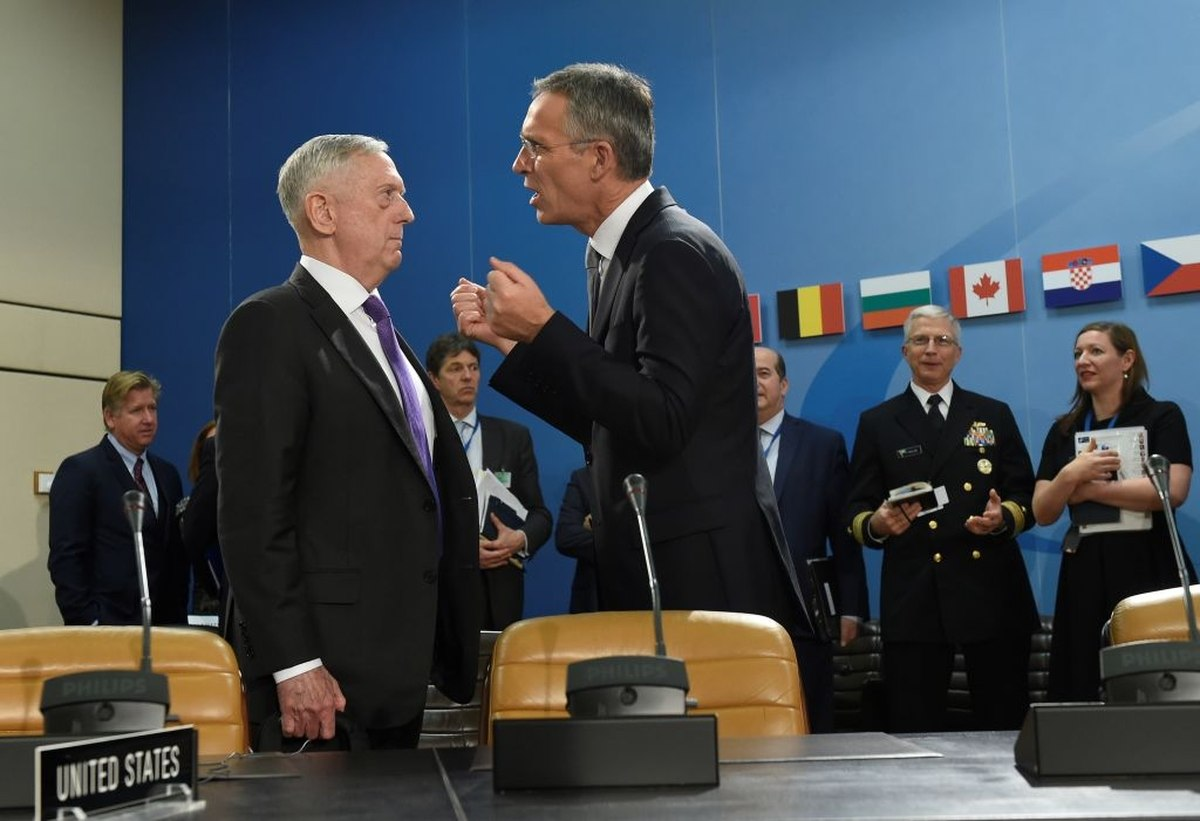
\includegraphics[width=0.95\textwidth]{mattis-nato.jpg}
	\label{fig:mattis-nato}
\end{figure}


\end{frame}


%------------------------------------------------

\begin{frame}[standout] 

\begin{figure}[htbp]
	\centering
		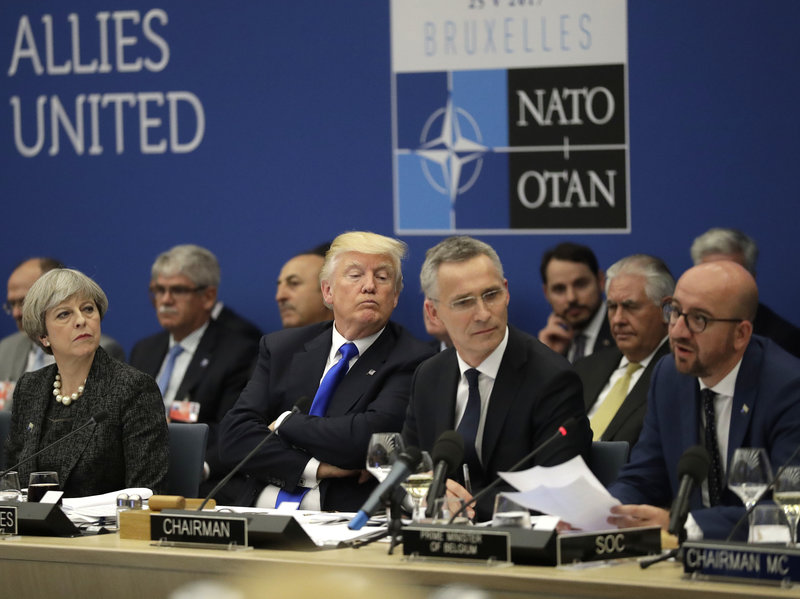
\includegraphics[width=0.95\textwidth]{trump-nato.jpg}
	\label{fig:trump-nato}
\end{figure}


\end{frame}
 


%------------------------------------------------

\begin{frame}{Outline}

I make my claim about alliance participation and military spending in three ways: 

\pause
\begin{enumerate}
\item Argument: Treaty Depth and Non-Major Powers
\pause
\item Statistical Analysis
\pause
\item Evidence from US alliances
\end{enumerate}


\end{frame}

%------------------------------------------------

\section{Argument}


%------------------------------------------------

\begin{frame}{An Alliance Politics Framework}

Alliances are a form of international cooperation. 
\begin{enumerate} 
\pause
\item States use allied support and capability to advance their foreign policy goals. 
\pause
\item Two potential concerns: abandonment and low military spending. 
\end{enumerate}  

\end{frame}

%------------------------------------------------

\begin{frame}{Non-Major Powers}

\begin{itemize}
\item Foreign policy goal: immediate security.
\pause
\item Constraint: Opportunity costs of military spending.  
\pause
\item Given the chance, alliance participation \emph{decreases} military spending. 
\end{itemize} 

\end{frame}

%------------------------------------------------

\begin{frame}{Allies of Non-Major Powers}

Often prefer higher non-major power military spending. 

\begin{enumerate} 
\pause
\item Adds capability to advance FP goals and manage internal threats.  
\pause
\item Hard to enforce- need leverage. 
\pause 
\item Leverage depends on a credible threat of abandonment.  
\pause 
\item Tradeoff between credible military support and leverage.

\end{enumerate}  

\end{frame}

%------------------------------------------------

\begin{frame}{Treaty Depth}

\pause 
Deep treaties stipulate extensive defense cooperation. 

\begin{enumerate} 
\pause
\item Require more policy coordination and defense cooperation among alliance members. 
\item \textbf{Formal defense cooperation}:
\pause
\begin{itemize}
\item Bases, policy coordination, military aid, side agreements, formal institutions. 
\end{itemize}  
\end{enumerate}  

\end{frame}


%------------------------------------------------

\begin{frame}{Depth, Credibility and Leverage}

Treaty depth shapes alliance politics in three ways: 

\begin{enumerate}
\pause
\item Greater alliance credibility and less fear of abandonment.   
\pause
\item Reduced leverage over allied spending.
\pause
\item Efficiency gains in defense spending. 
\end{enumerate}

\end{frame}


%------------------------------------------------

\begin{frame}{Hypotheses 1 and 2} 

\begin{quote}
\textsc{Hypothesis 1: On average, participation in shallow alliances will increase percentage changes in non-major power military spending.}
\end{quote}
\pause

\begin{quote}
\textsc{Hypothesis 2: On average, participation in deep alliances will decrease percentage changes in non-major power military spending.}
\end{quote}

\end{frame}

%------------------------------------------------

\begin{frame}{Hypothesis 3} 

\begin{quote}
\textsc{Hypothesis 3: As alliance treaty depth increases, the impact of alliance participation on percentage changes in non-major power military spending will decrease.}
\end{quote}

\end{frame}

%------------------------------------------------

\section{Empirical Analysis} 

%-----------------------------------------------

\begin{frame}{Research Design}

I need two things to test these predictions: 

\pause 
\begin{enumerate} 
\item Measure of treaty depth--- measurement model. 
\pause
\item Connect alliance-level variation with state-level outcomes--- multilevel Bayesian analysis.  
\end{enumerate} 


\end{frame}

%------------------------------------------------

\begin{frame}{Measuring Treaty Depth}

I use a latent variable model to infer treaty depth from observed promises. 

\pause 

My measure of depth for each alliance is the posterior mean of the latent depth factor. 

\end{frame} 

%------------------------------------------------

\begin{frame}{Details of Measure}
 
\begin{itemize}
\item Multiple observed indicators of depth in ATOP alliances with military support: 
\begin{itemize} 
\item \textit{Defense Cooperation}: bases, integrated command, military aid, IO formation, defense policy coordination, other military agreements, subordination of forces, specific contribution. 
\end{itemize} 
\pause 
\item Semiparametric mixed factor analysis. (Murray et al 2013)
\end{itemize} 


\end{frame} 

%------------------------------------------------

\begin{frame}{Factor Loadings}


\begin{figure}
	\centering
		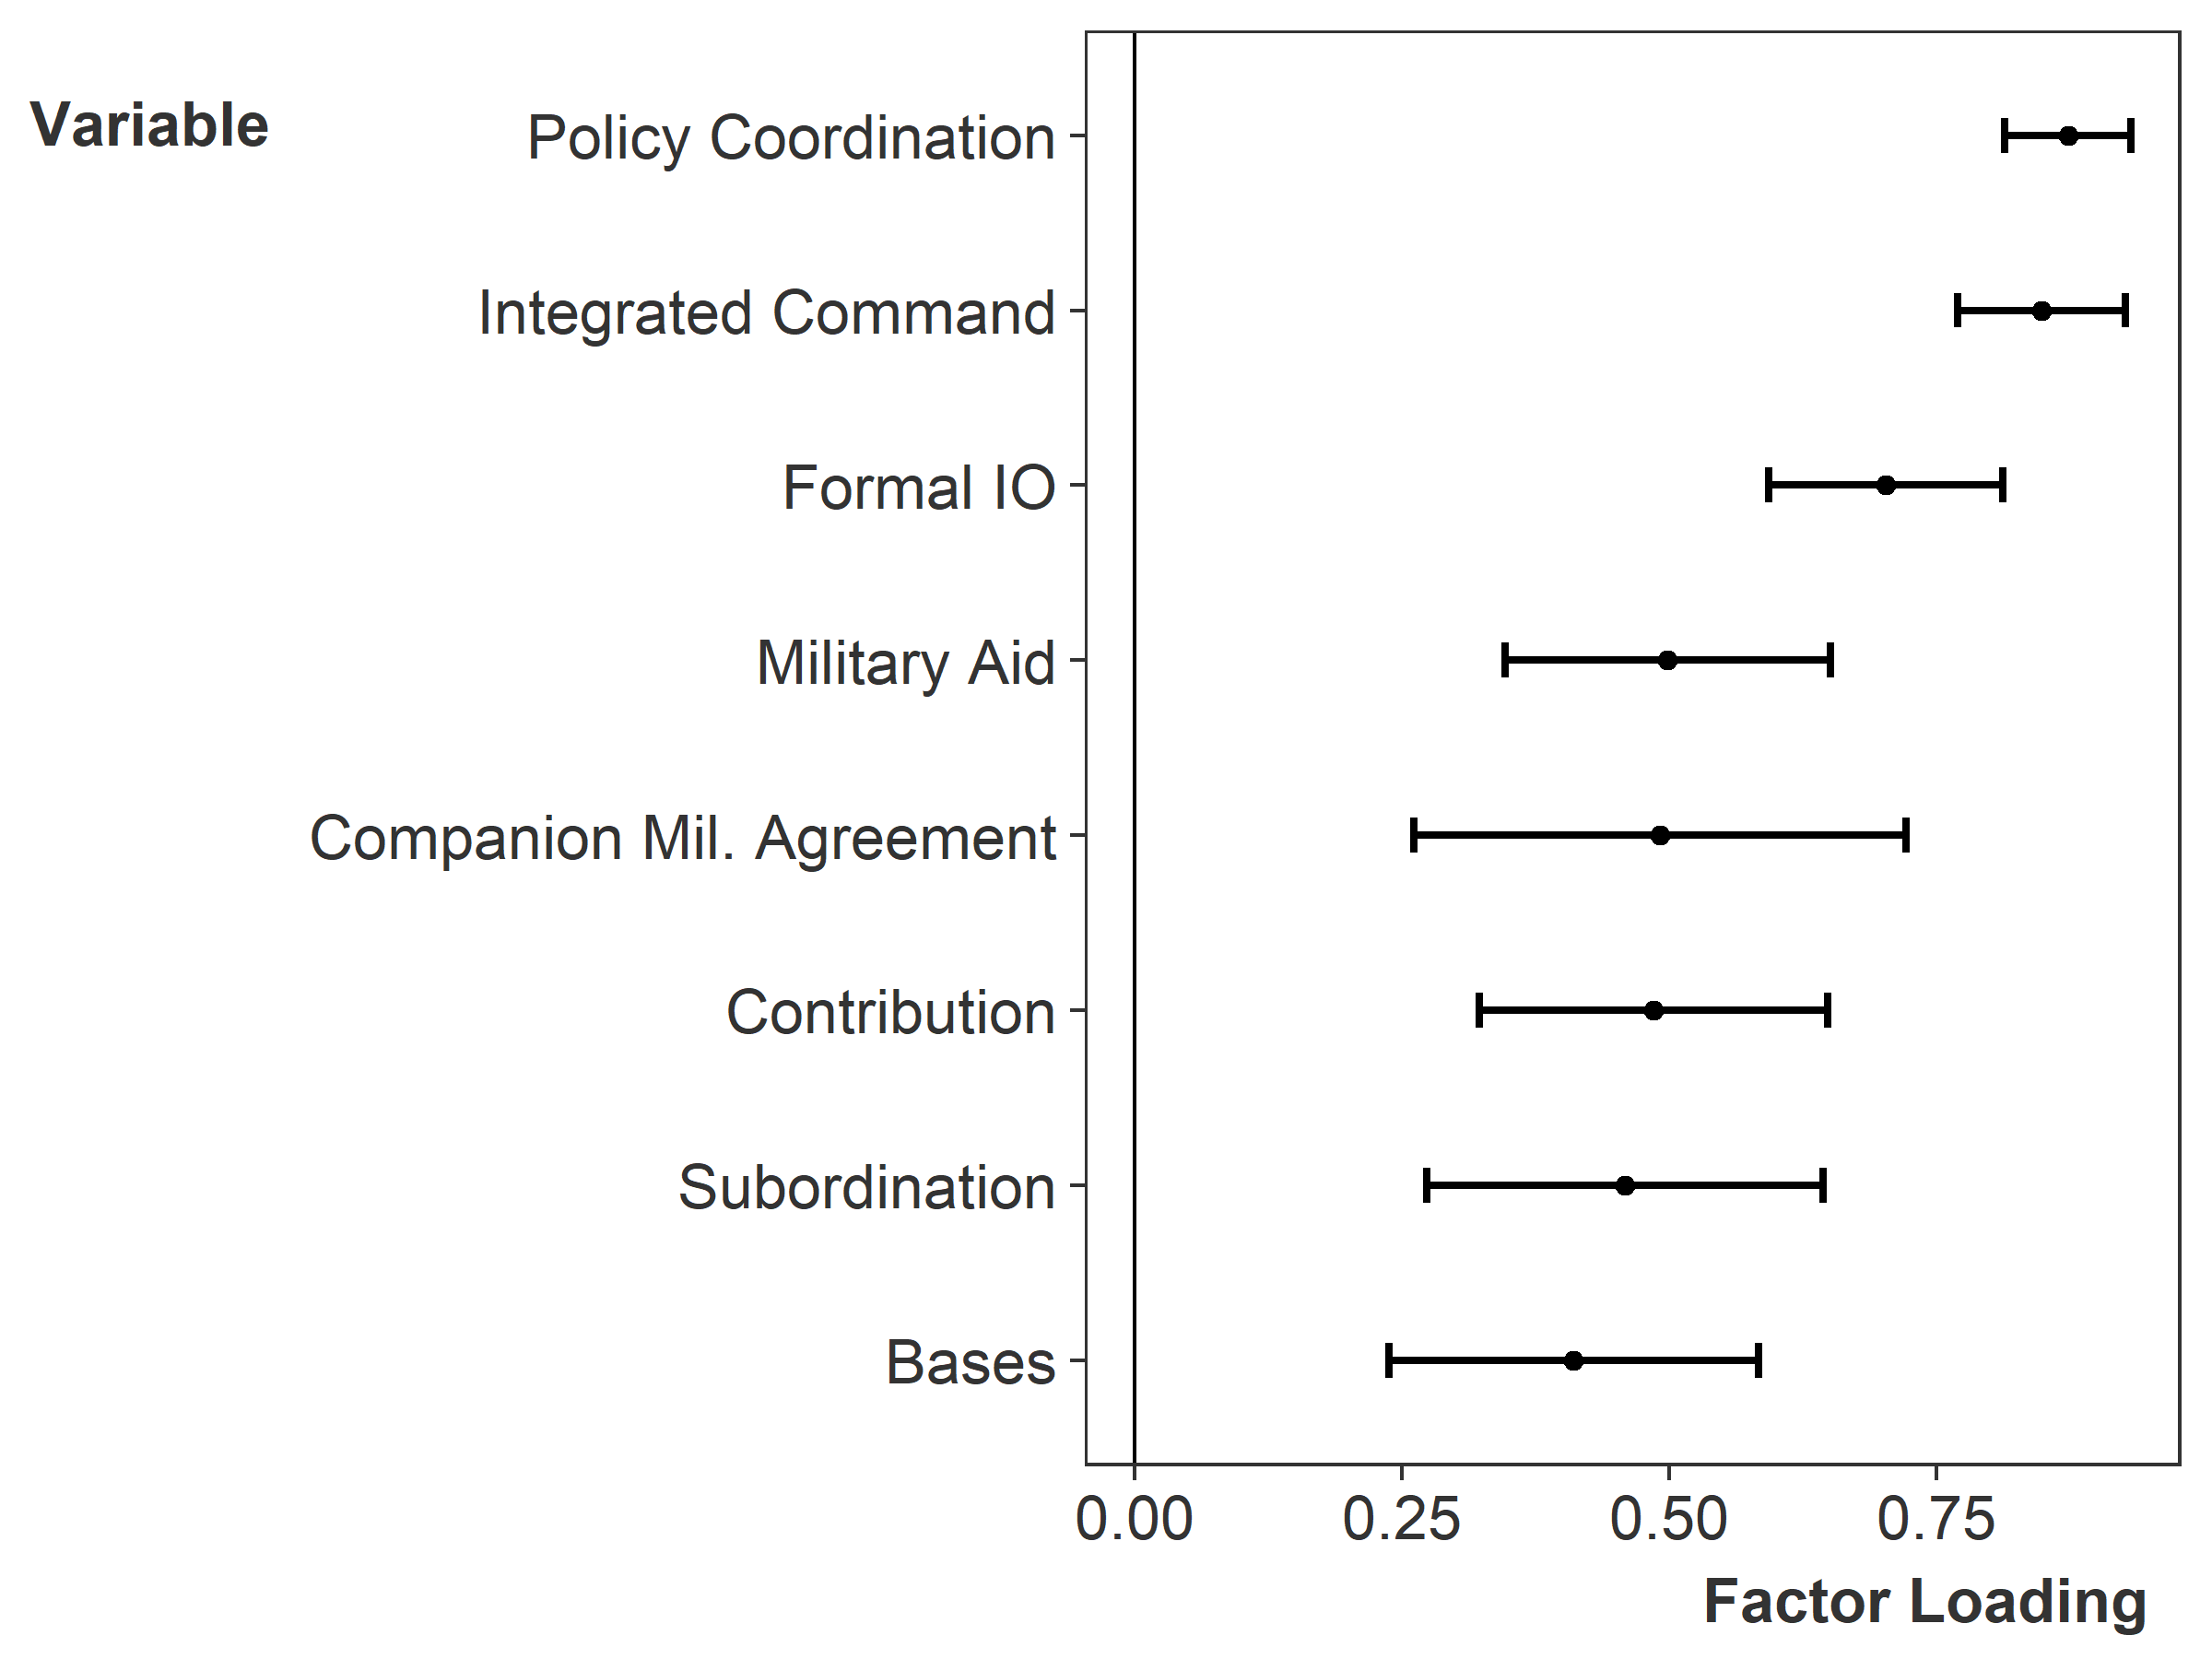
\includegraphics[width=0.95\textwidth]{factor-loadings.png}
\end{figure}


\end{frame}

%------------------------------------------------

\begin{frame}{Latent Measure of Treaty Depth}

% Visual summary of latent measure
\begin{figure}[htbp]
	\centering
		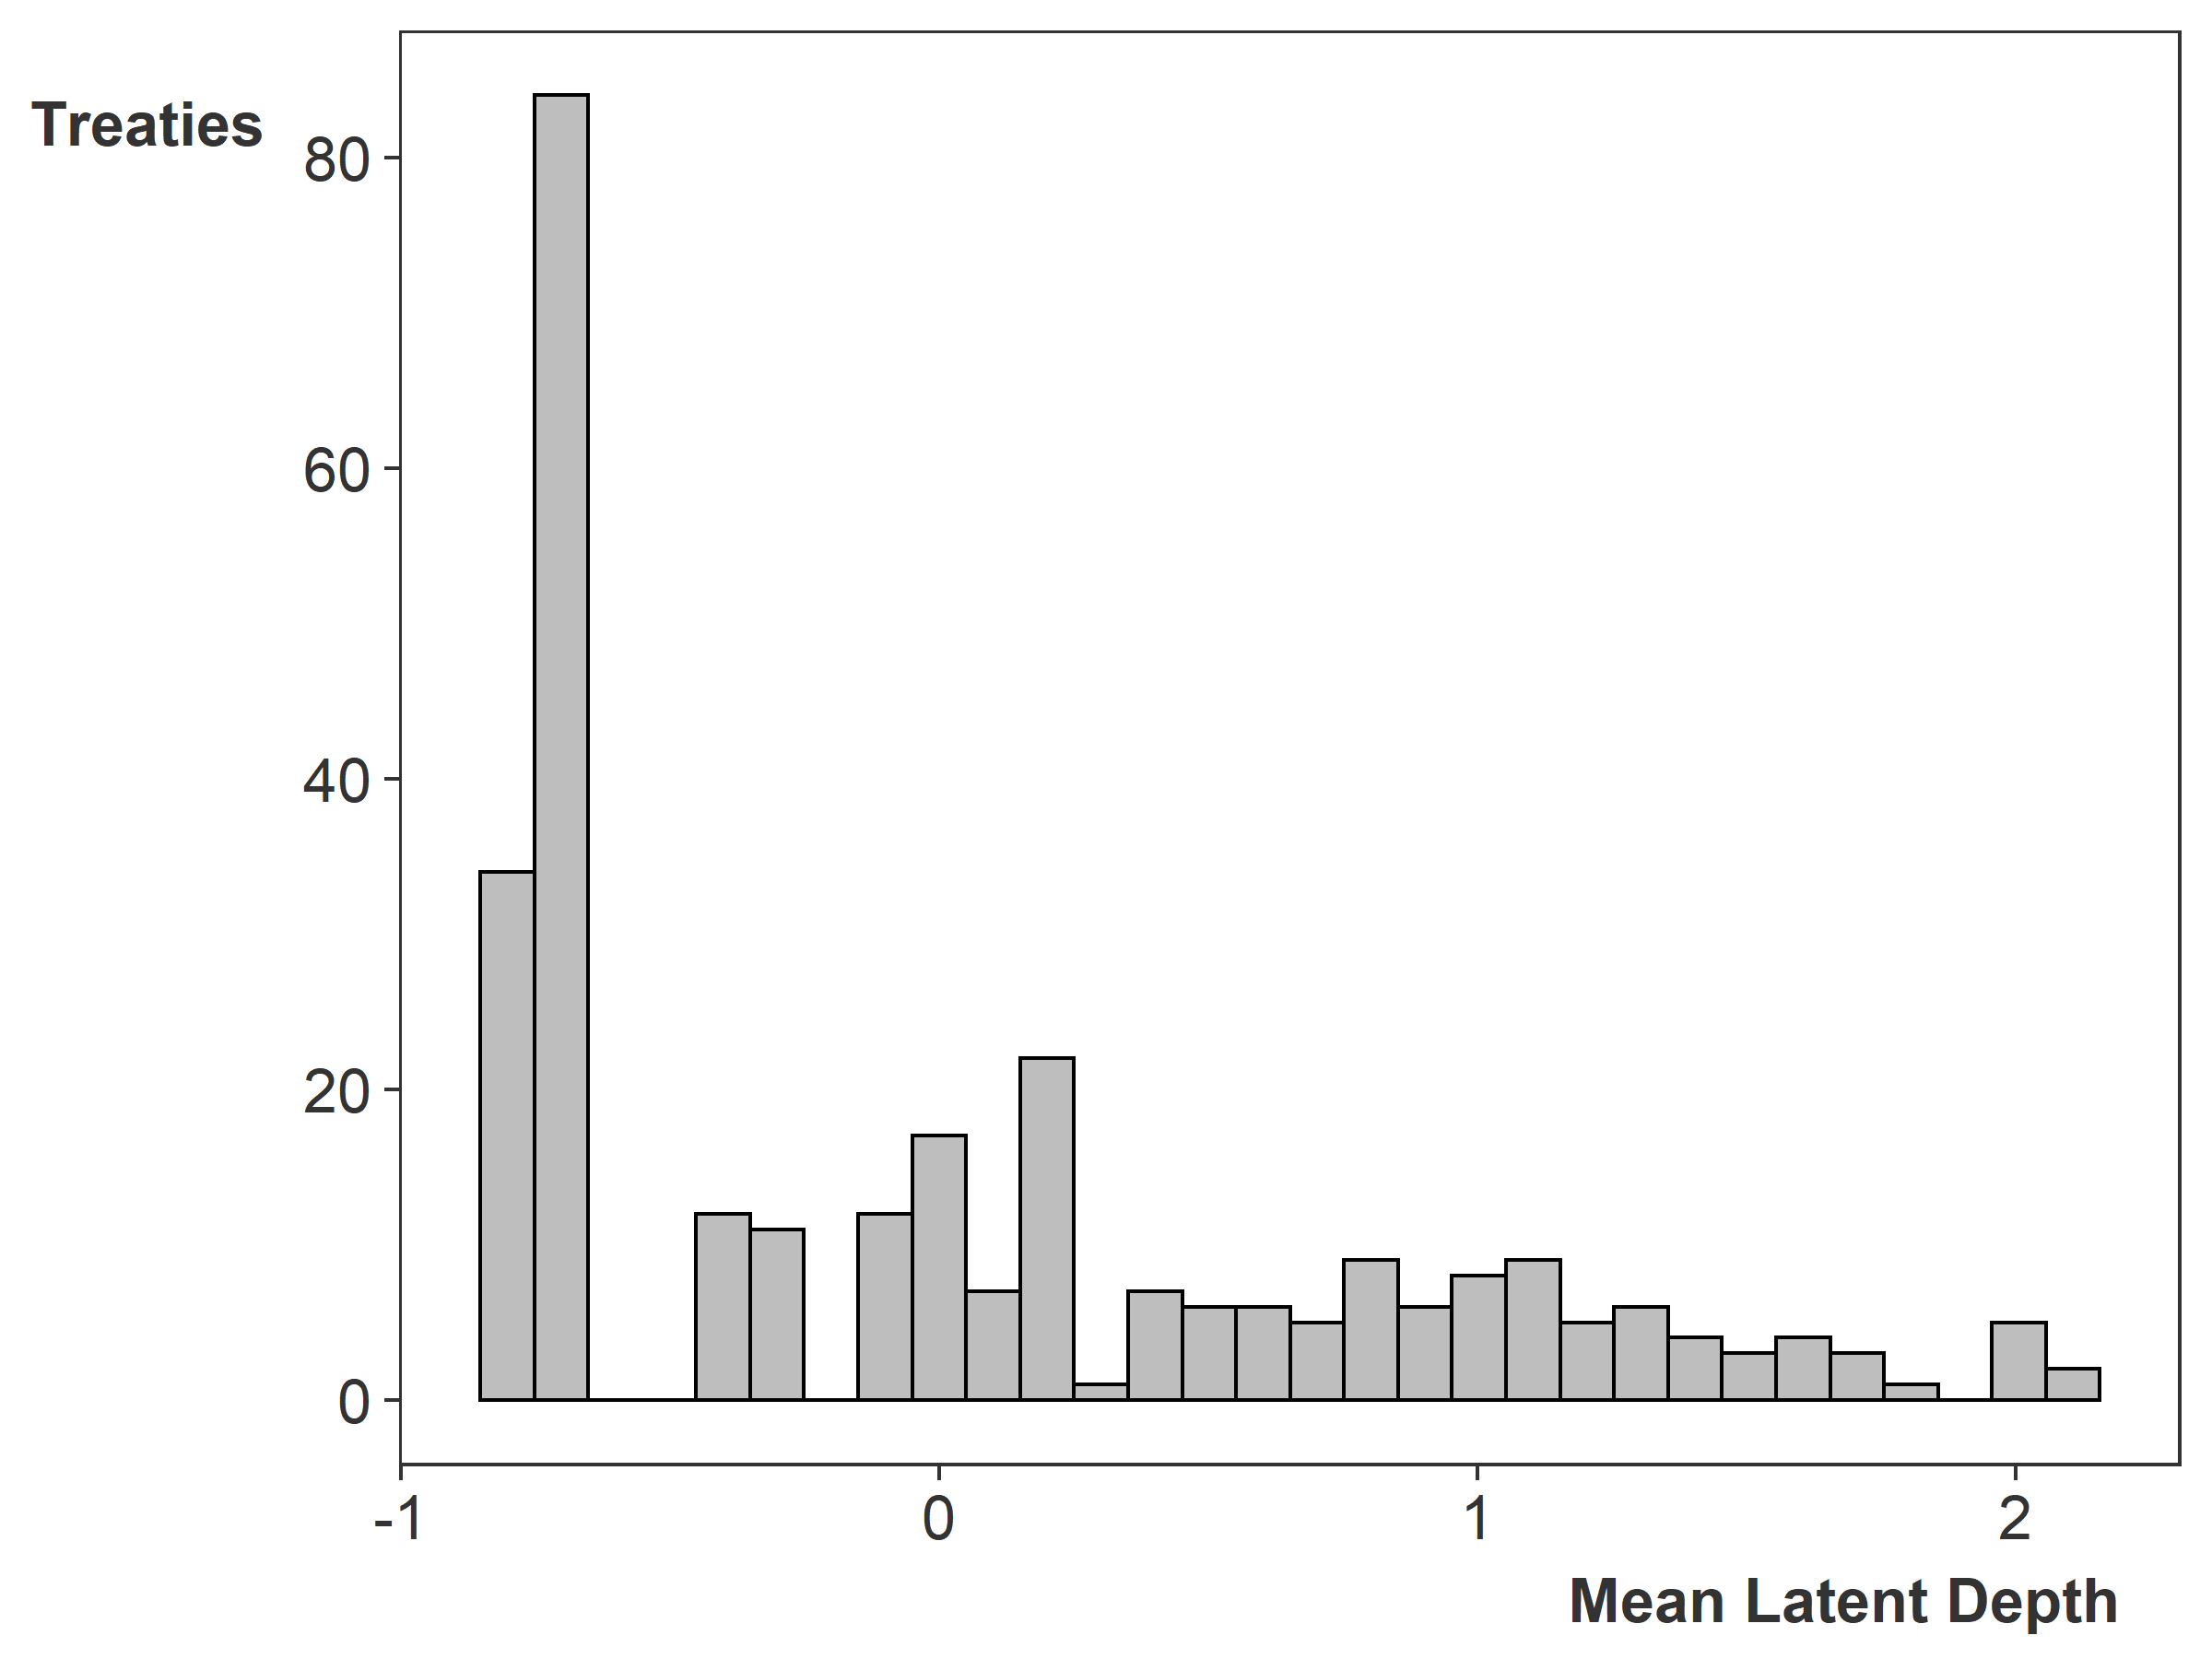
\includegraphics[width=0.95\textwidth]{ld-hist.png}
\end{figure}


\end{frame} 

%------------------------------------------------

\begin{frame}{Latent Measure of Treaty Depth: Shallow}

% Visual summary of latent measure
\begin{figure}[htbp]
	\centering
		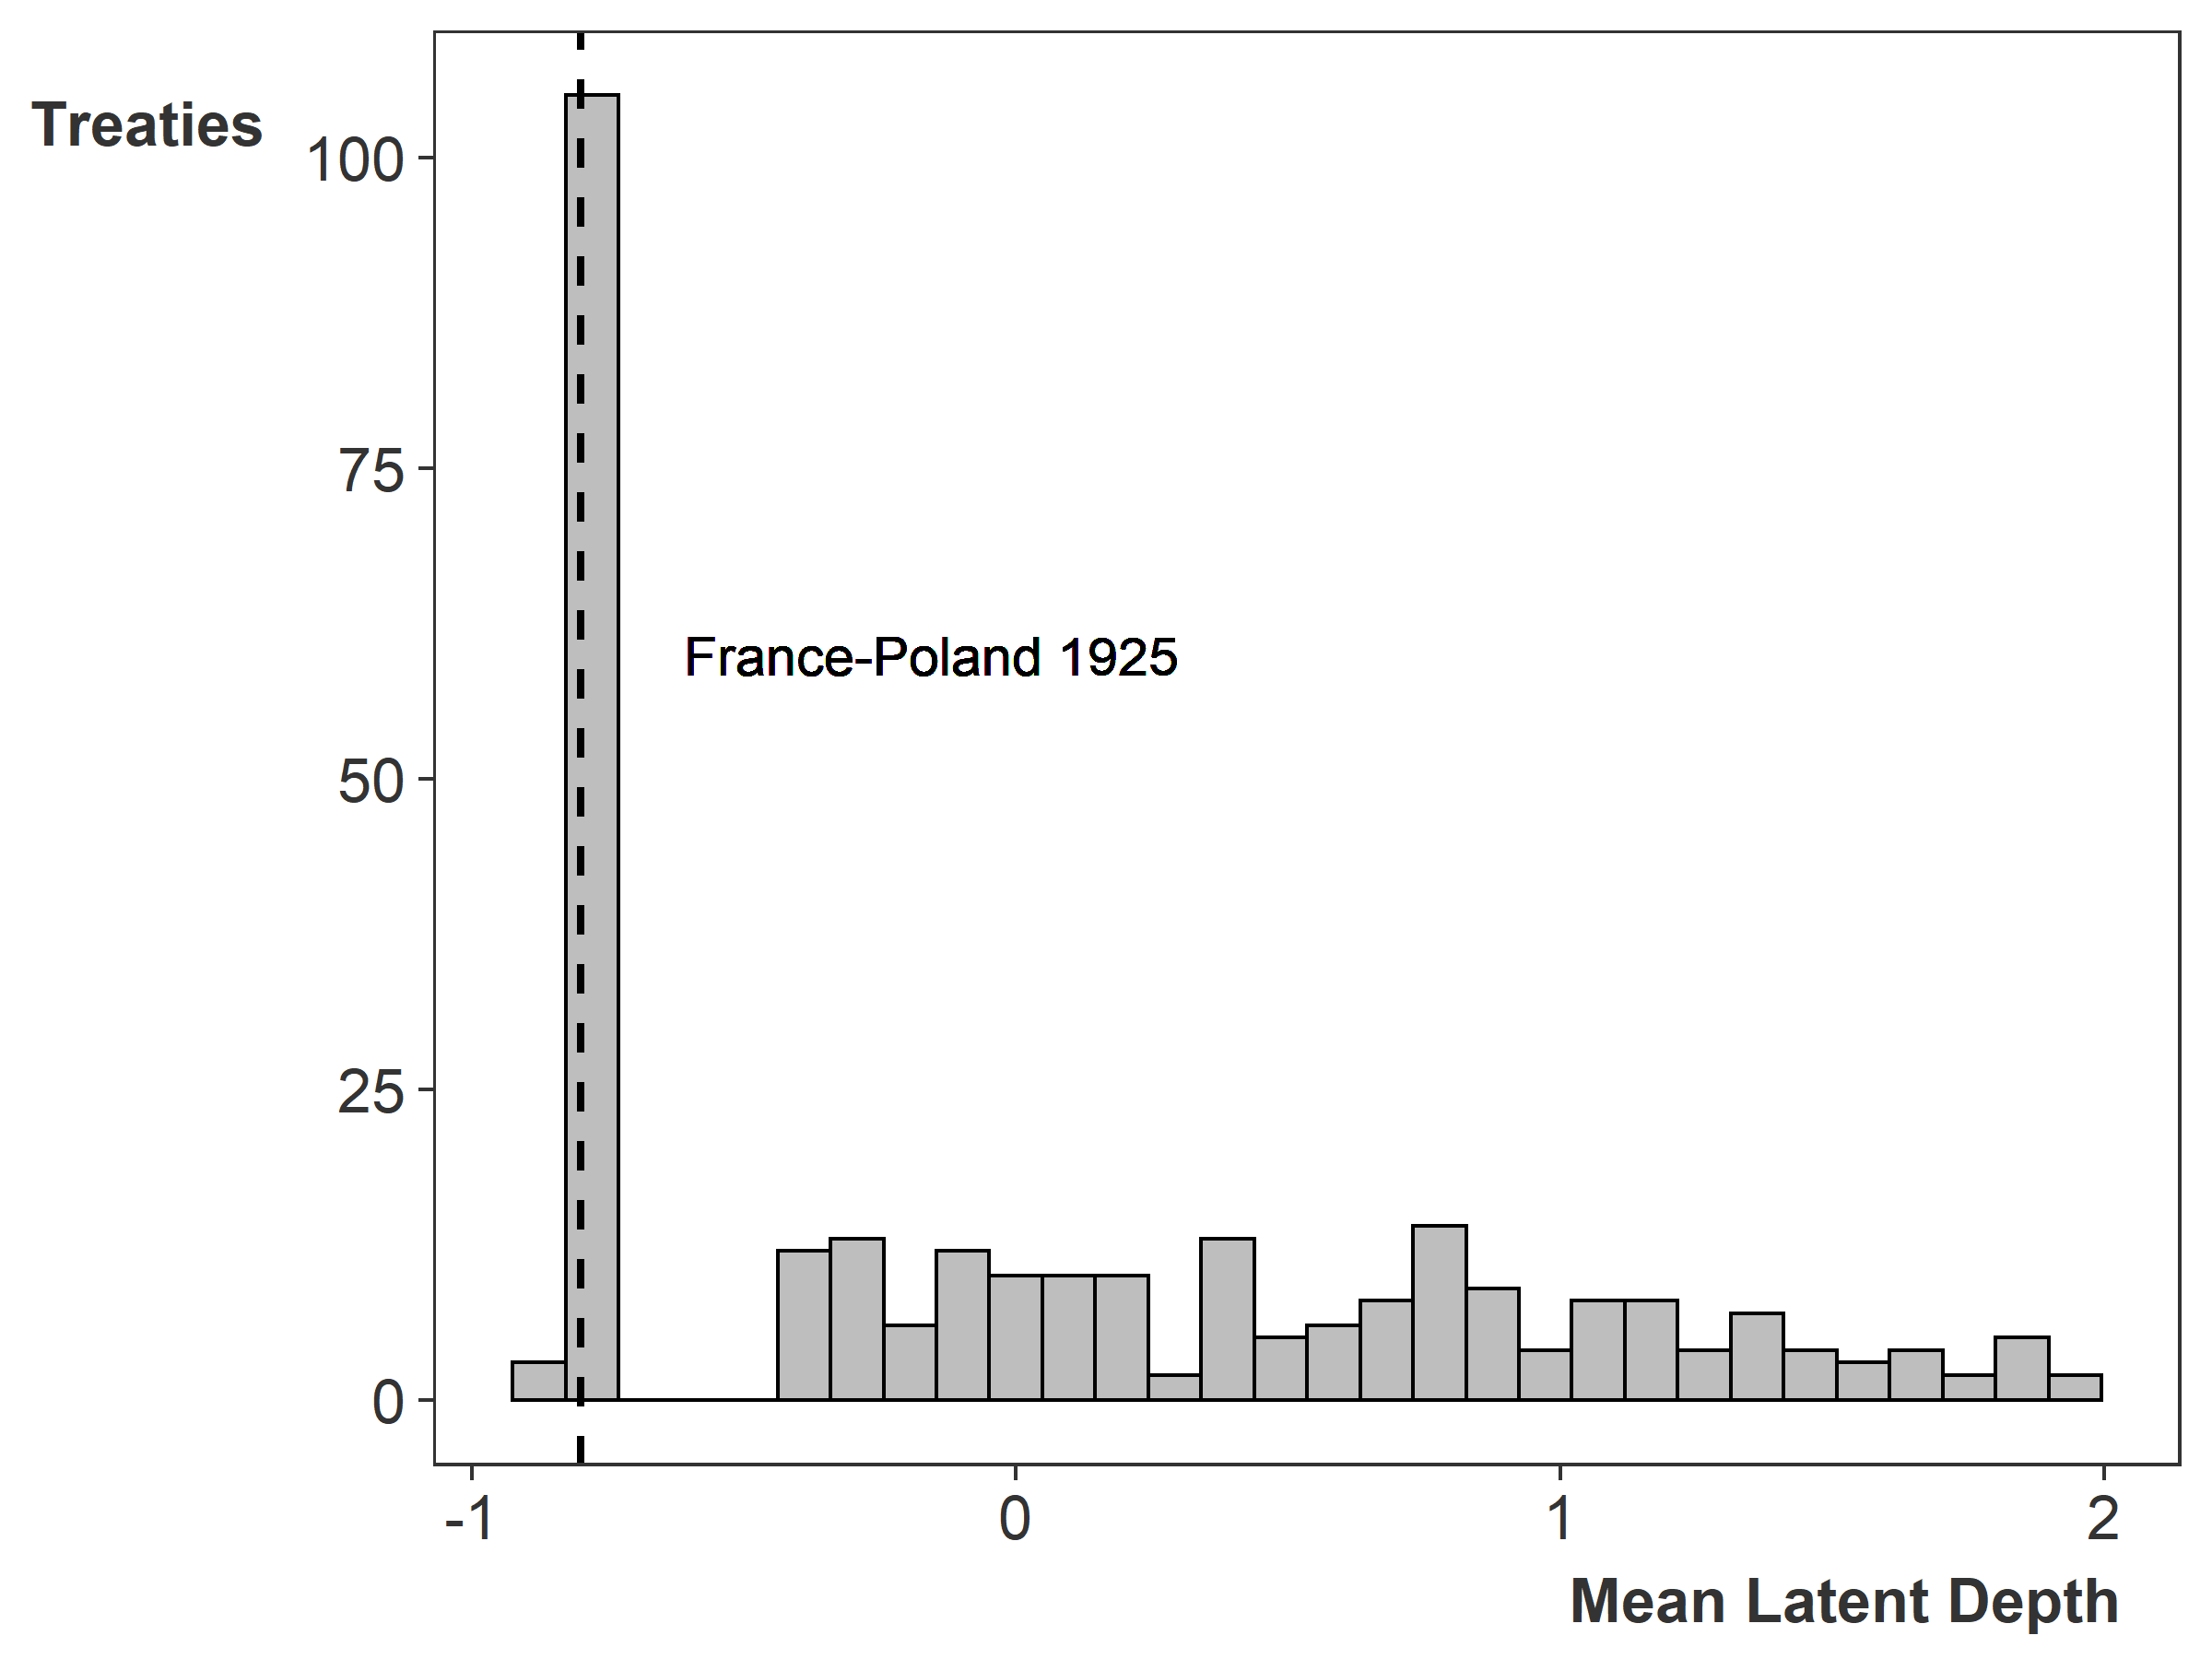
\includegraphics[width=0.95\textwidth]{ld-hist-shallow.png}
\end{figure}


\end{frame} 

%------------------------------------------------

\begin{frame}{Latent Measure of Treaty Depth: Typical}

% Visual summary of latent measure
\begin{figure}[htbp]
	\centering
		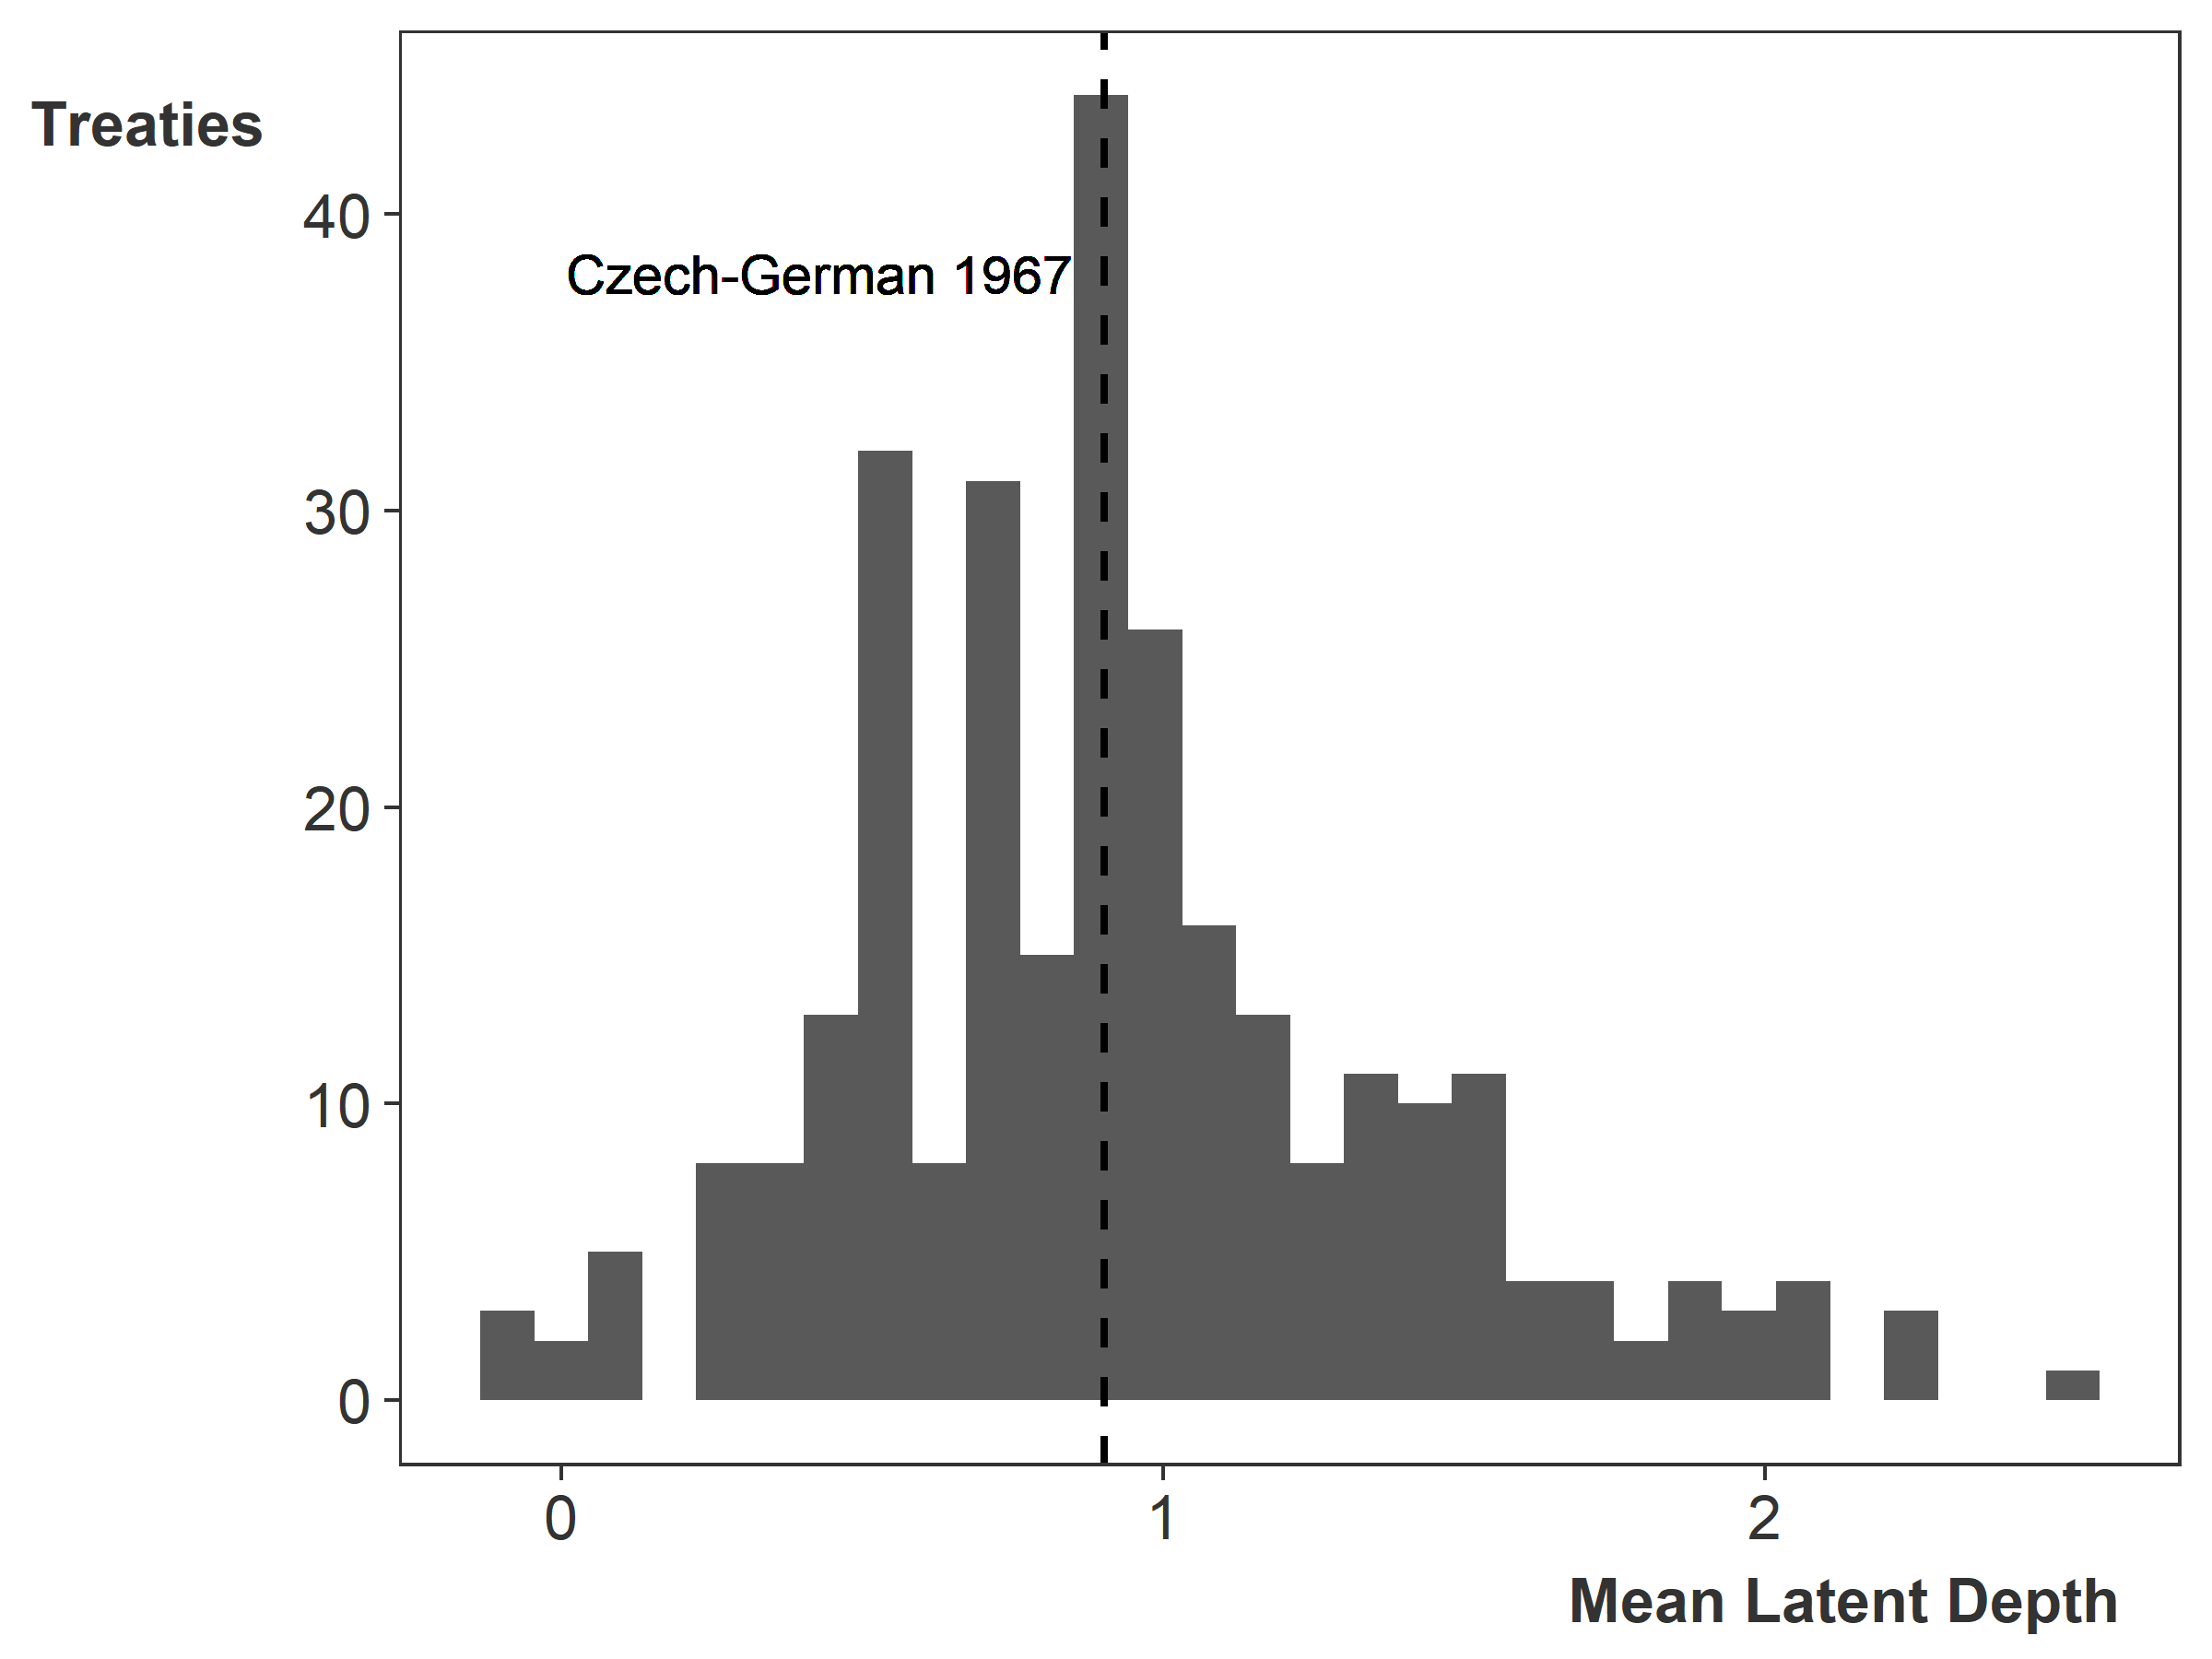
\includegraphics[width=0.95\textwidth]{ld-hist-median.png}
\end{figure}


\end{frame} 

%------------------------------------------------

\begin{frame}{Latent Measure of Treaty Depth: Deep}

% Visual summary of latent measure
\begin{figure}[htbp]
	\centering
		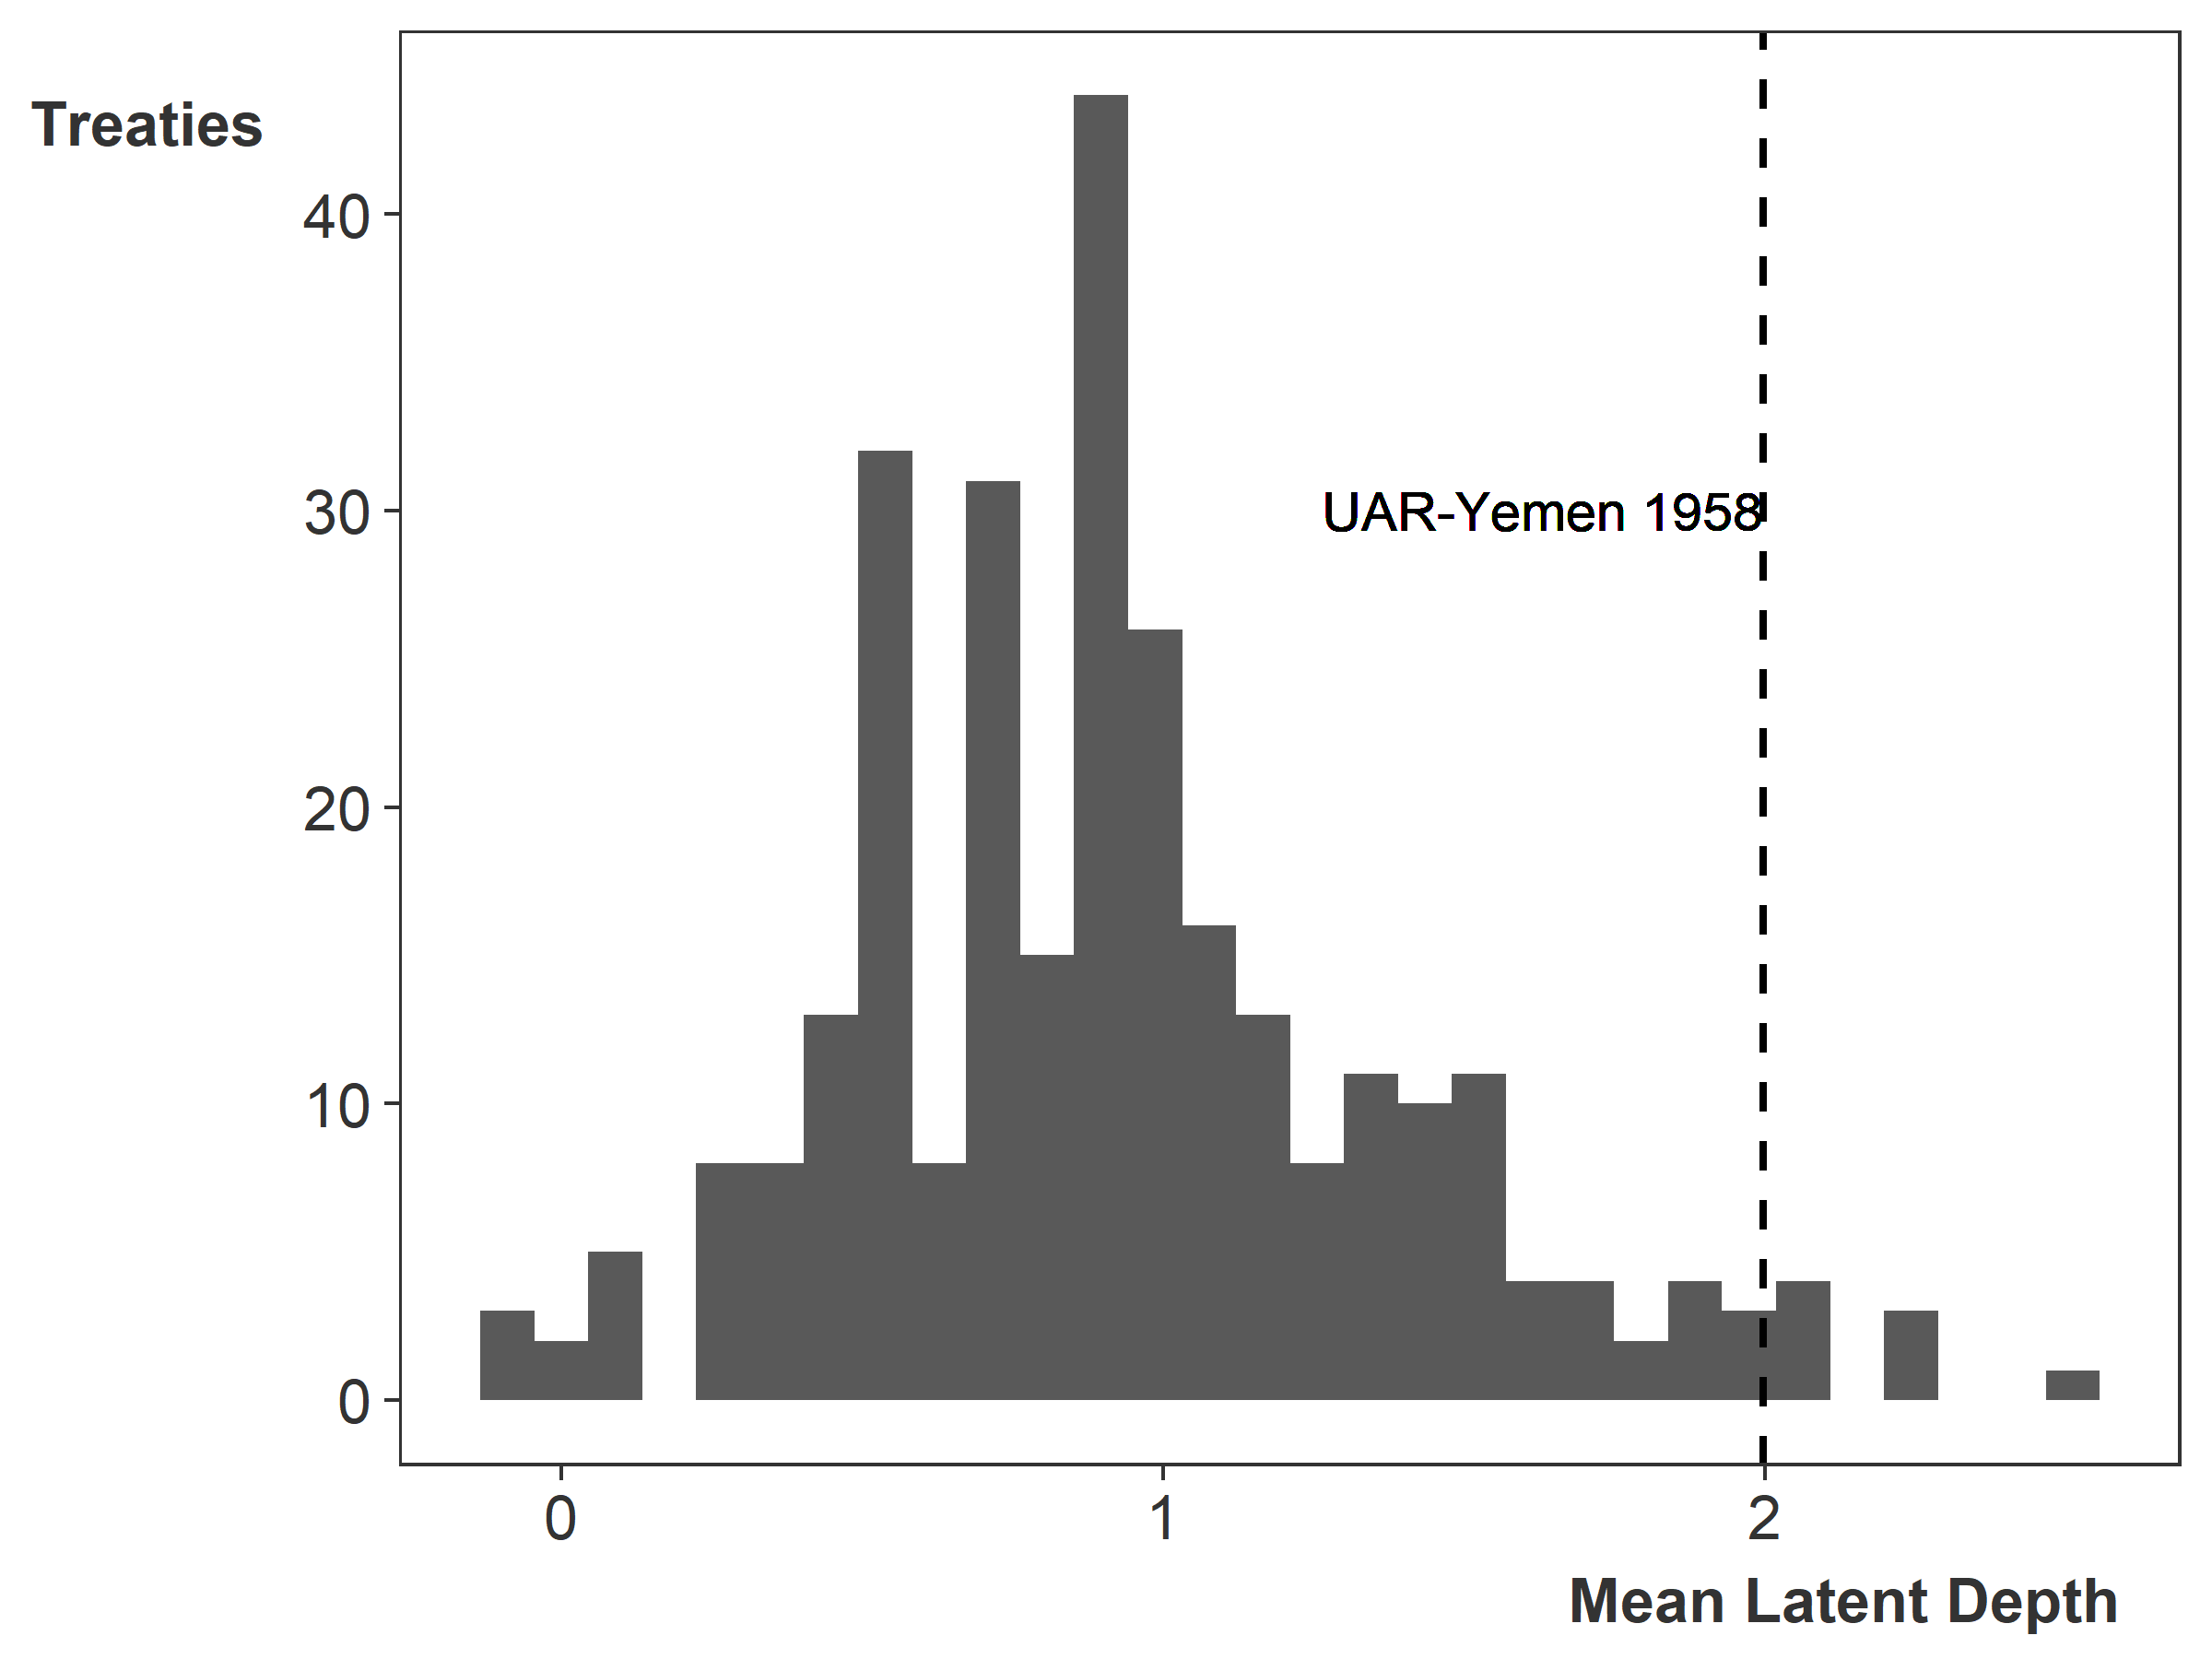
\includegraphics[width=0.95\textwidth]{ld-hist-deep.png}
\end{figure}


\end{frame} 


%------------------------------------------------

\begin{frame}{Empirical Analysis: Multilevel Model}

\begin{itemize} 
\item Link alliance-level variation with state-level outcomes. 
\pause
\item Two connected regressions: alliance and state-level. 
\pause 
\item Alliance characteristics modify the association between alliance membership and percentage changes in spending.  
\end{itemize} 

\end{frame} 


%------------------------------------------------

\begin{frame}{Why Multilevel?}

\begin{enumerate} 
\item Matches the theoretical argument by comparing alliances. 
\pause
\item Explicitly model heterogeneous effects of alliances.
\pause
\item States are members of multiple alliances.  
\pause 
\item Includes multiple salient alliance characteristics. 
\end{enumerate} 

\end{frame} 


%------------------------------------------------

\begin{frame}{ML Model}

\[
\begin{array}{cccccc}
\uncover<2->{ & & & & &\mbox{Alliance} \\
& & & & &    \mbox{Characteristics}  \\
& & & & &    \downarrow \uncover<3->{\mbox{Depth -}}  \\}
\mbox{\% Change} =     & \mbox{Varying}   & + & \mbox{State}   & + & \mbox{Alliance} \\
\mbox{Mil. Ex.}      & \mbox{Intercepts}&   &  \mbox{Vars.} &   & \mbox{Participation} \\
\end{array}
\]


\end{frame}

%------------------------------------------------

\begin{frame}{ML Model}

\[
\begin{array}{cccccc}
 & & & & &      \mbox{Alliance} \\
& & & & &    \mbox{Characteristics}  \\
\uncover<3->{& & & & \lambda = & \beta_1 \mbox{Depth} + \textbf{X} \beta \\}
& & & & &    \downarrow  \\
\mbox{\% Change} =     & \mbox{Varying}   & + & \mbox{State}   & + & \mbox{Alliance} \\
\mbox{Mil. Ex.}      & \mbox{Intercepts}&   &  \mbox{Vars.} &   & \mbox{Participation} \\
\uncover<2->{\mbox{y} = & \alpha + \alpha^{st} + \alpha^{yr}   & + & \textbf{W} \gamma  & + & \textbf{Z} \lambda \\}
\end{array}
\]


\end{frame}


%------------------------------------------------

\begin{frame}{Sample and Key Variables}

\begin{itemize}
\item \textbf{Sample}: Non-major power states (COW)--- 1816-2007. 
\pause 
\item 193 Alliances with military support: symmetric and asymmetric. 
\pause
\item \textbf{DV}: Percentage change in military spending (COW) $ = \frac{ \Delta \mbox{Mil. Expend}_t }{ \mbox{Mil. Expend}_{t-1} }$ 
\pause
\begin{itemize} 
\item Transformed with Inverse Hyperbolic Sine. 
\end{itemize} 
\pause
\item \textbf{Alliance-Level IV}: Mean treaty depth
\end{itemize} 

\end{frame}


%------------------------------------------------

\begin{frame}{Controls}

\begin{itemize}
\item \textbf{State-Level Controls}: Interstate war, civil war, annual MIDs, GDP growth, POLITY, Cold War, rival military expenditures. 
\pause 
\item \textbf{Alliance-Level Controls}: Unconditional military support, economic issue linkages, foreign policy concessions, share of democracies, number of members, wartime, asymmetric obligations, US member (Cold War), USSR member.

\end{itemize} 

\end{frame}


%------------------------------------------------

\subsection{Results}

%------------------------------------------------

\begin{frame}{Treaty Depth and the Impact of Alliance Participation} 

\begin{figure}
	\centering
		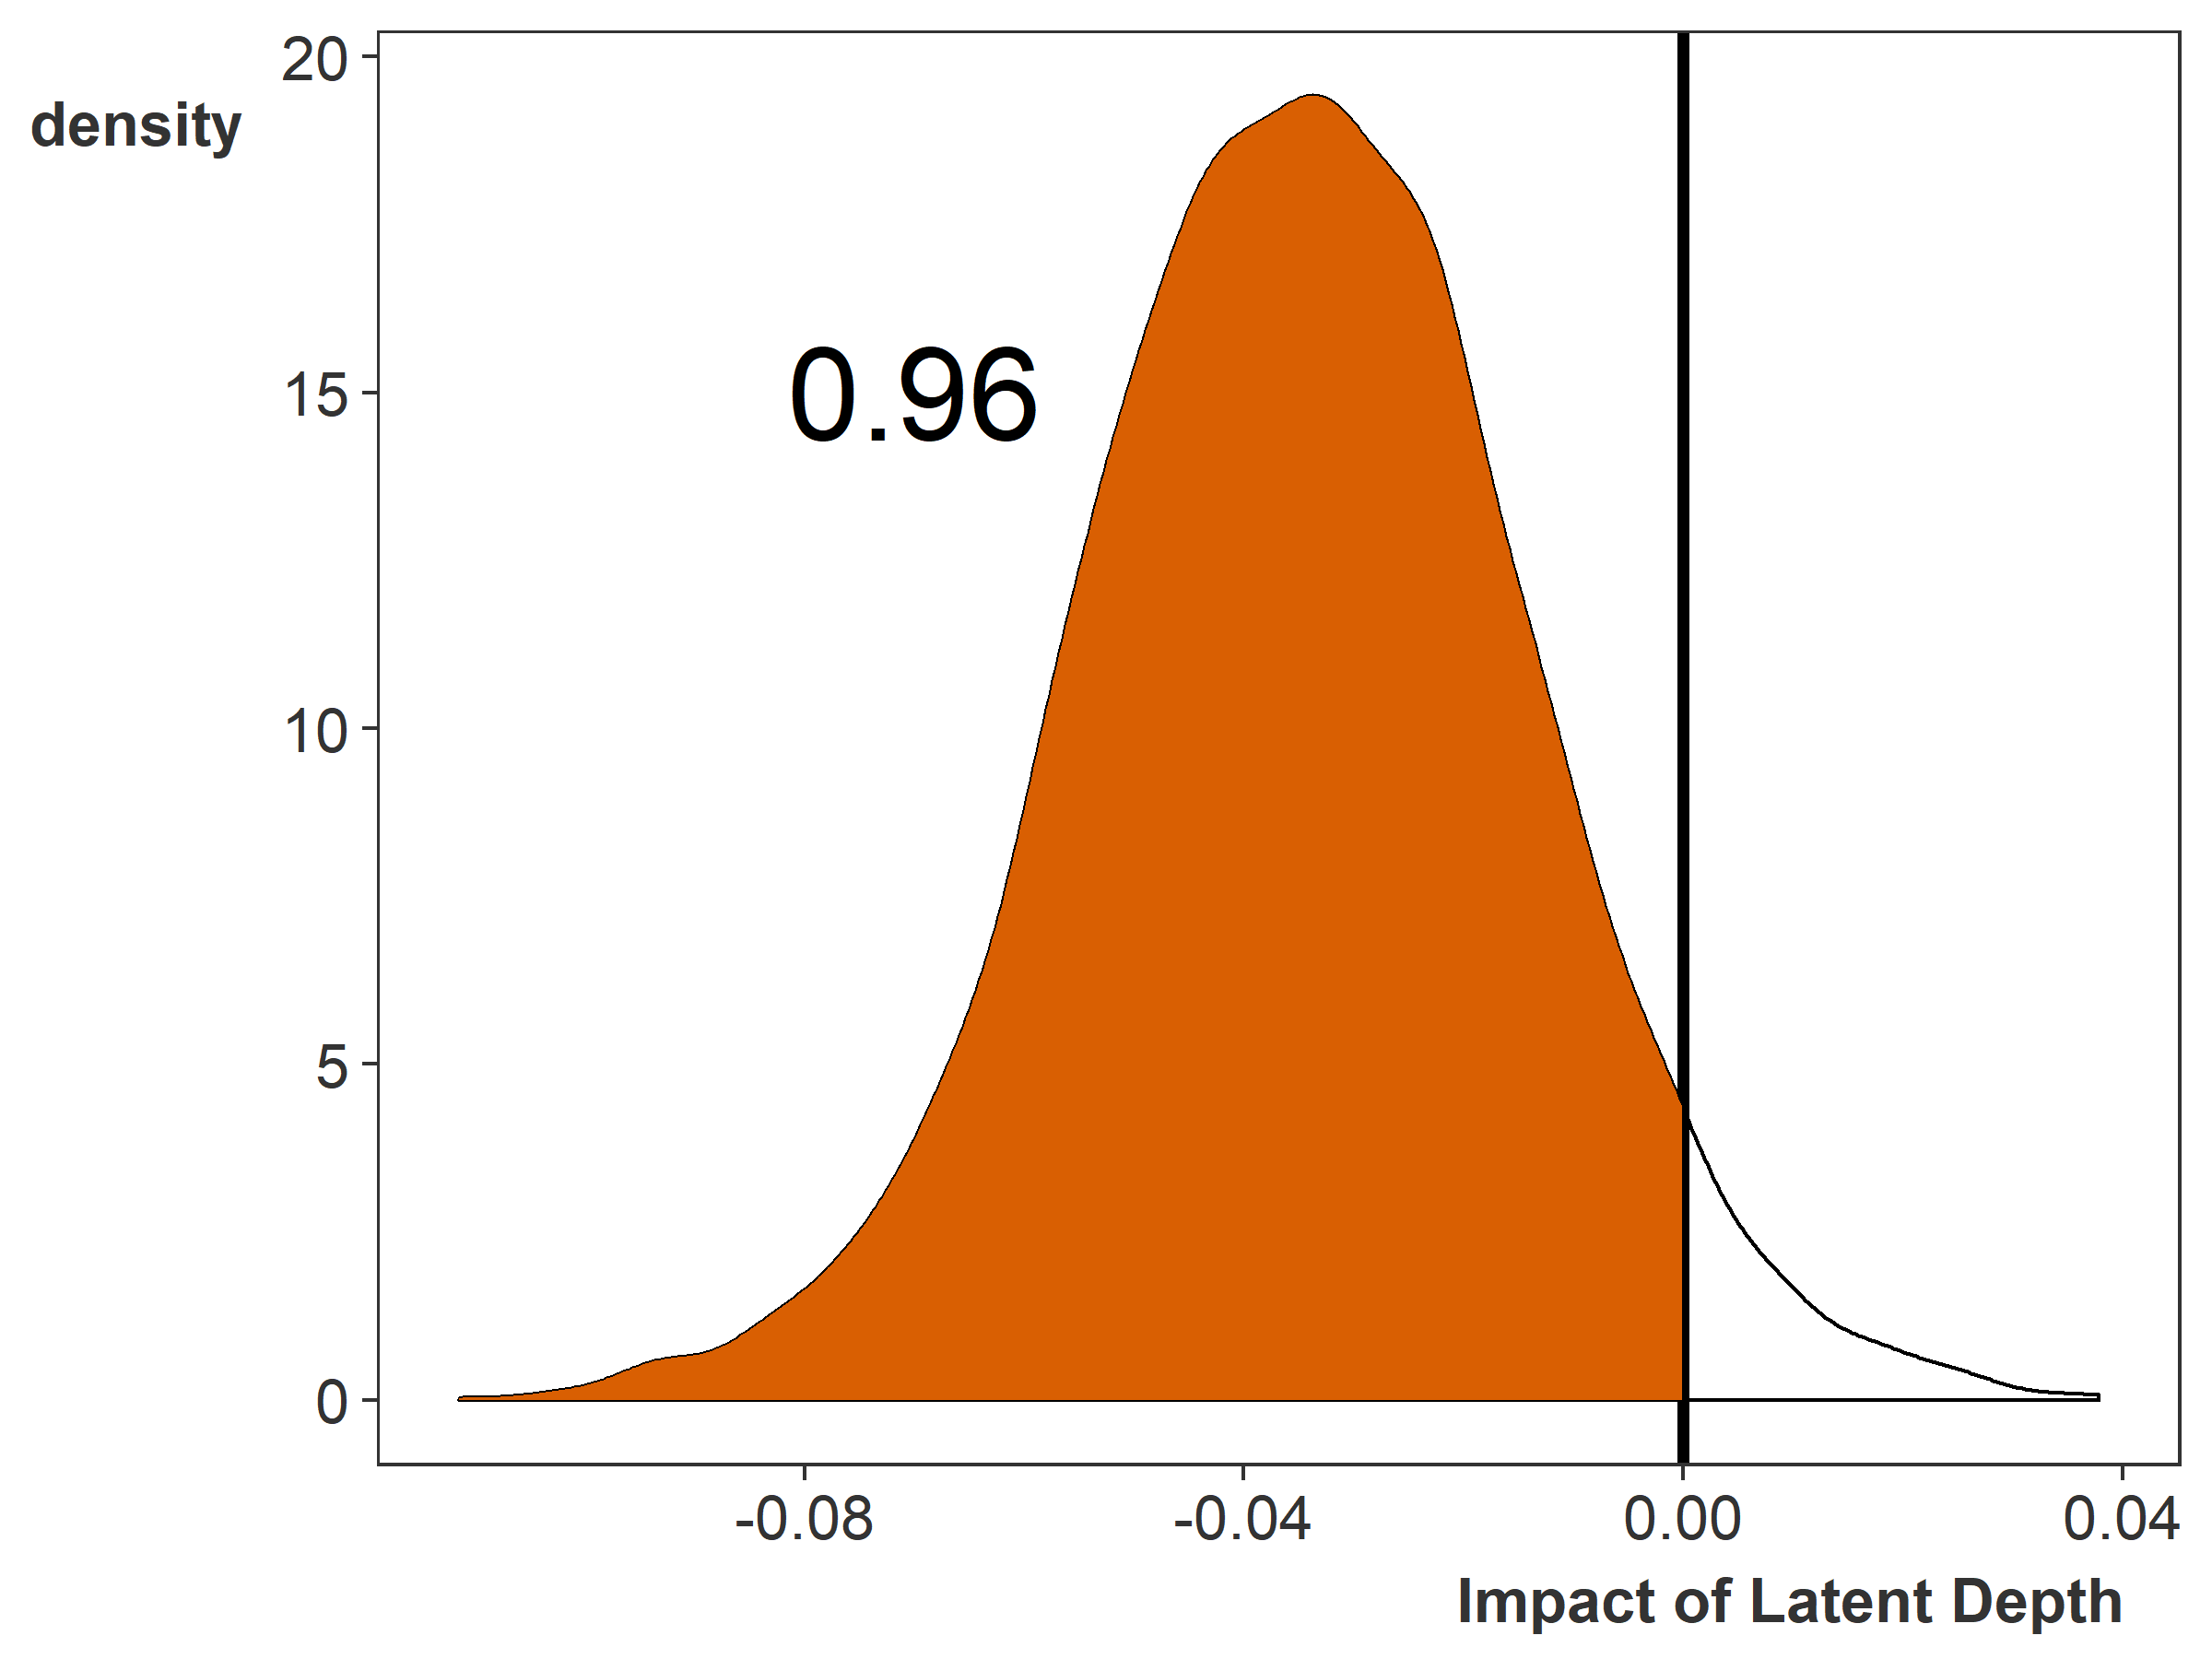
\includegraphics[width=0.90\textwidth]{depth-post.png}
	\label{fig:depth-post}
\end{figure}


\end{frame}


%------------------------------------------------

\begin{frame}{Substantive Importance} 

\pause 

\begin{figure}
	\centering
		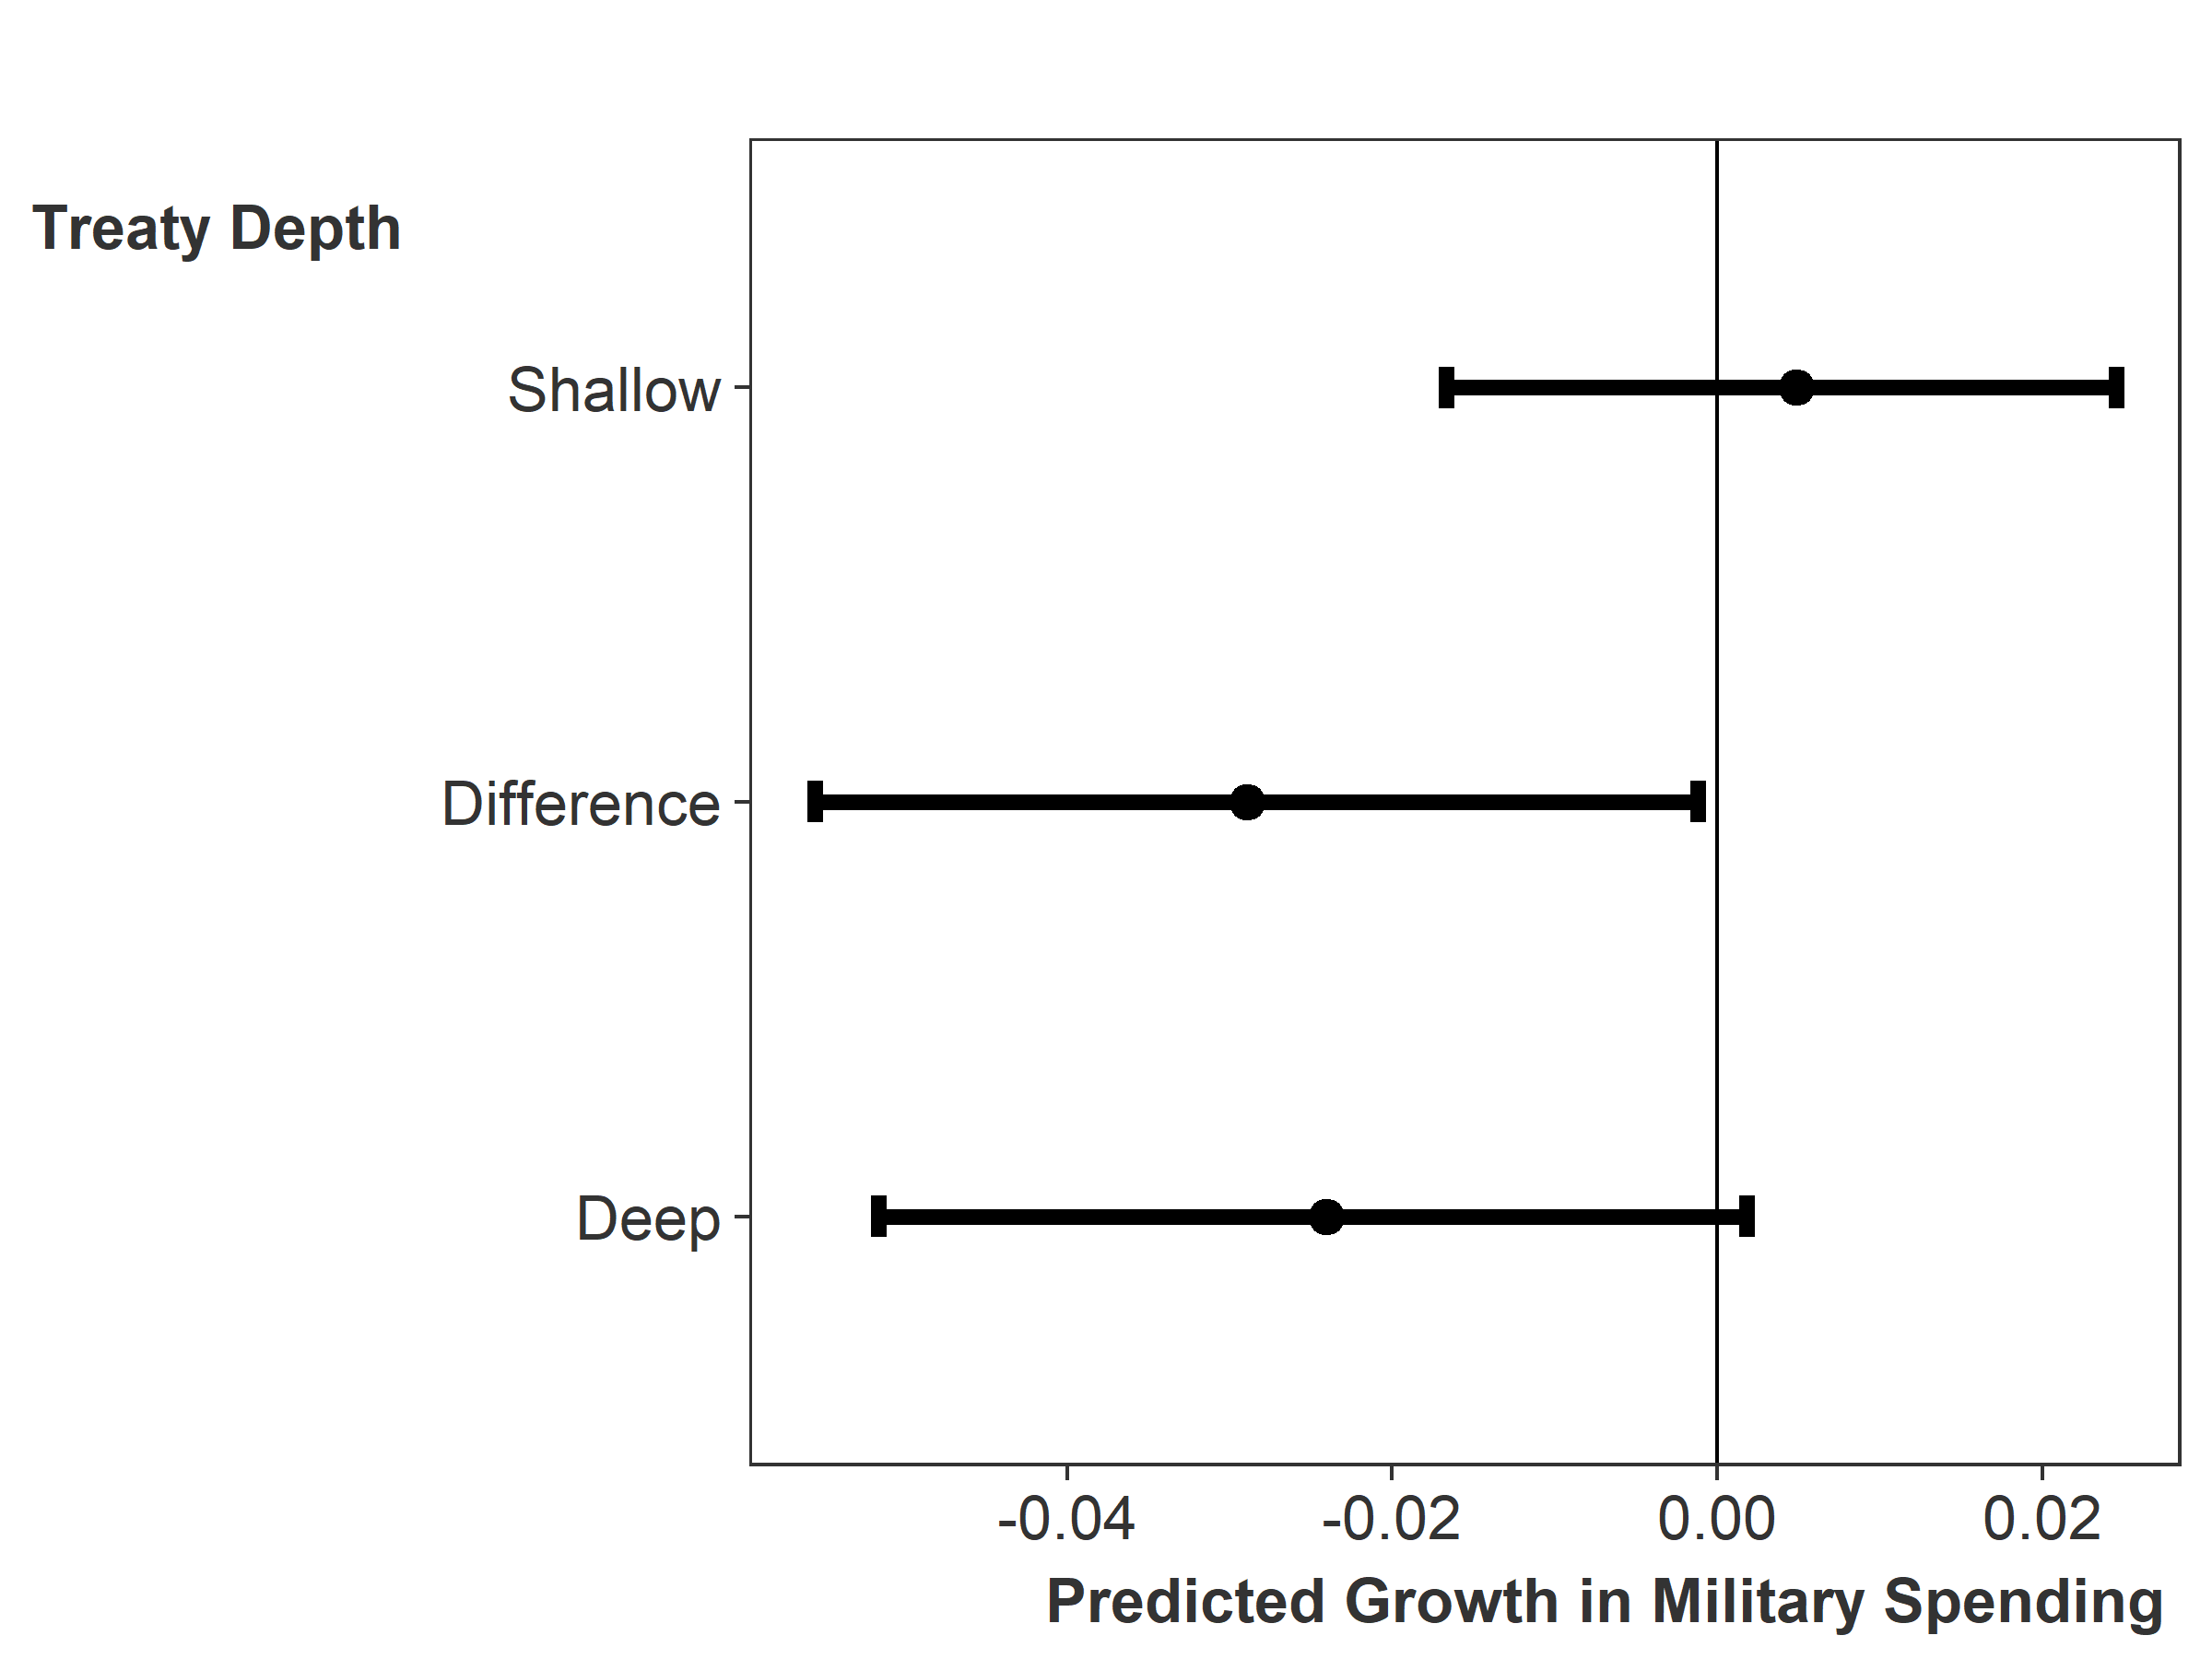
\includegraphics[width=0.95\textwidth]{pred-impact-depth.png}
\end{figure}

\end{frame}

%------------------------------------------------


\begin{frame}{How Treaty Depth Modifies Alliance Coefficients}

\begin{figure}[htbp]
	\centering
		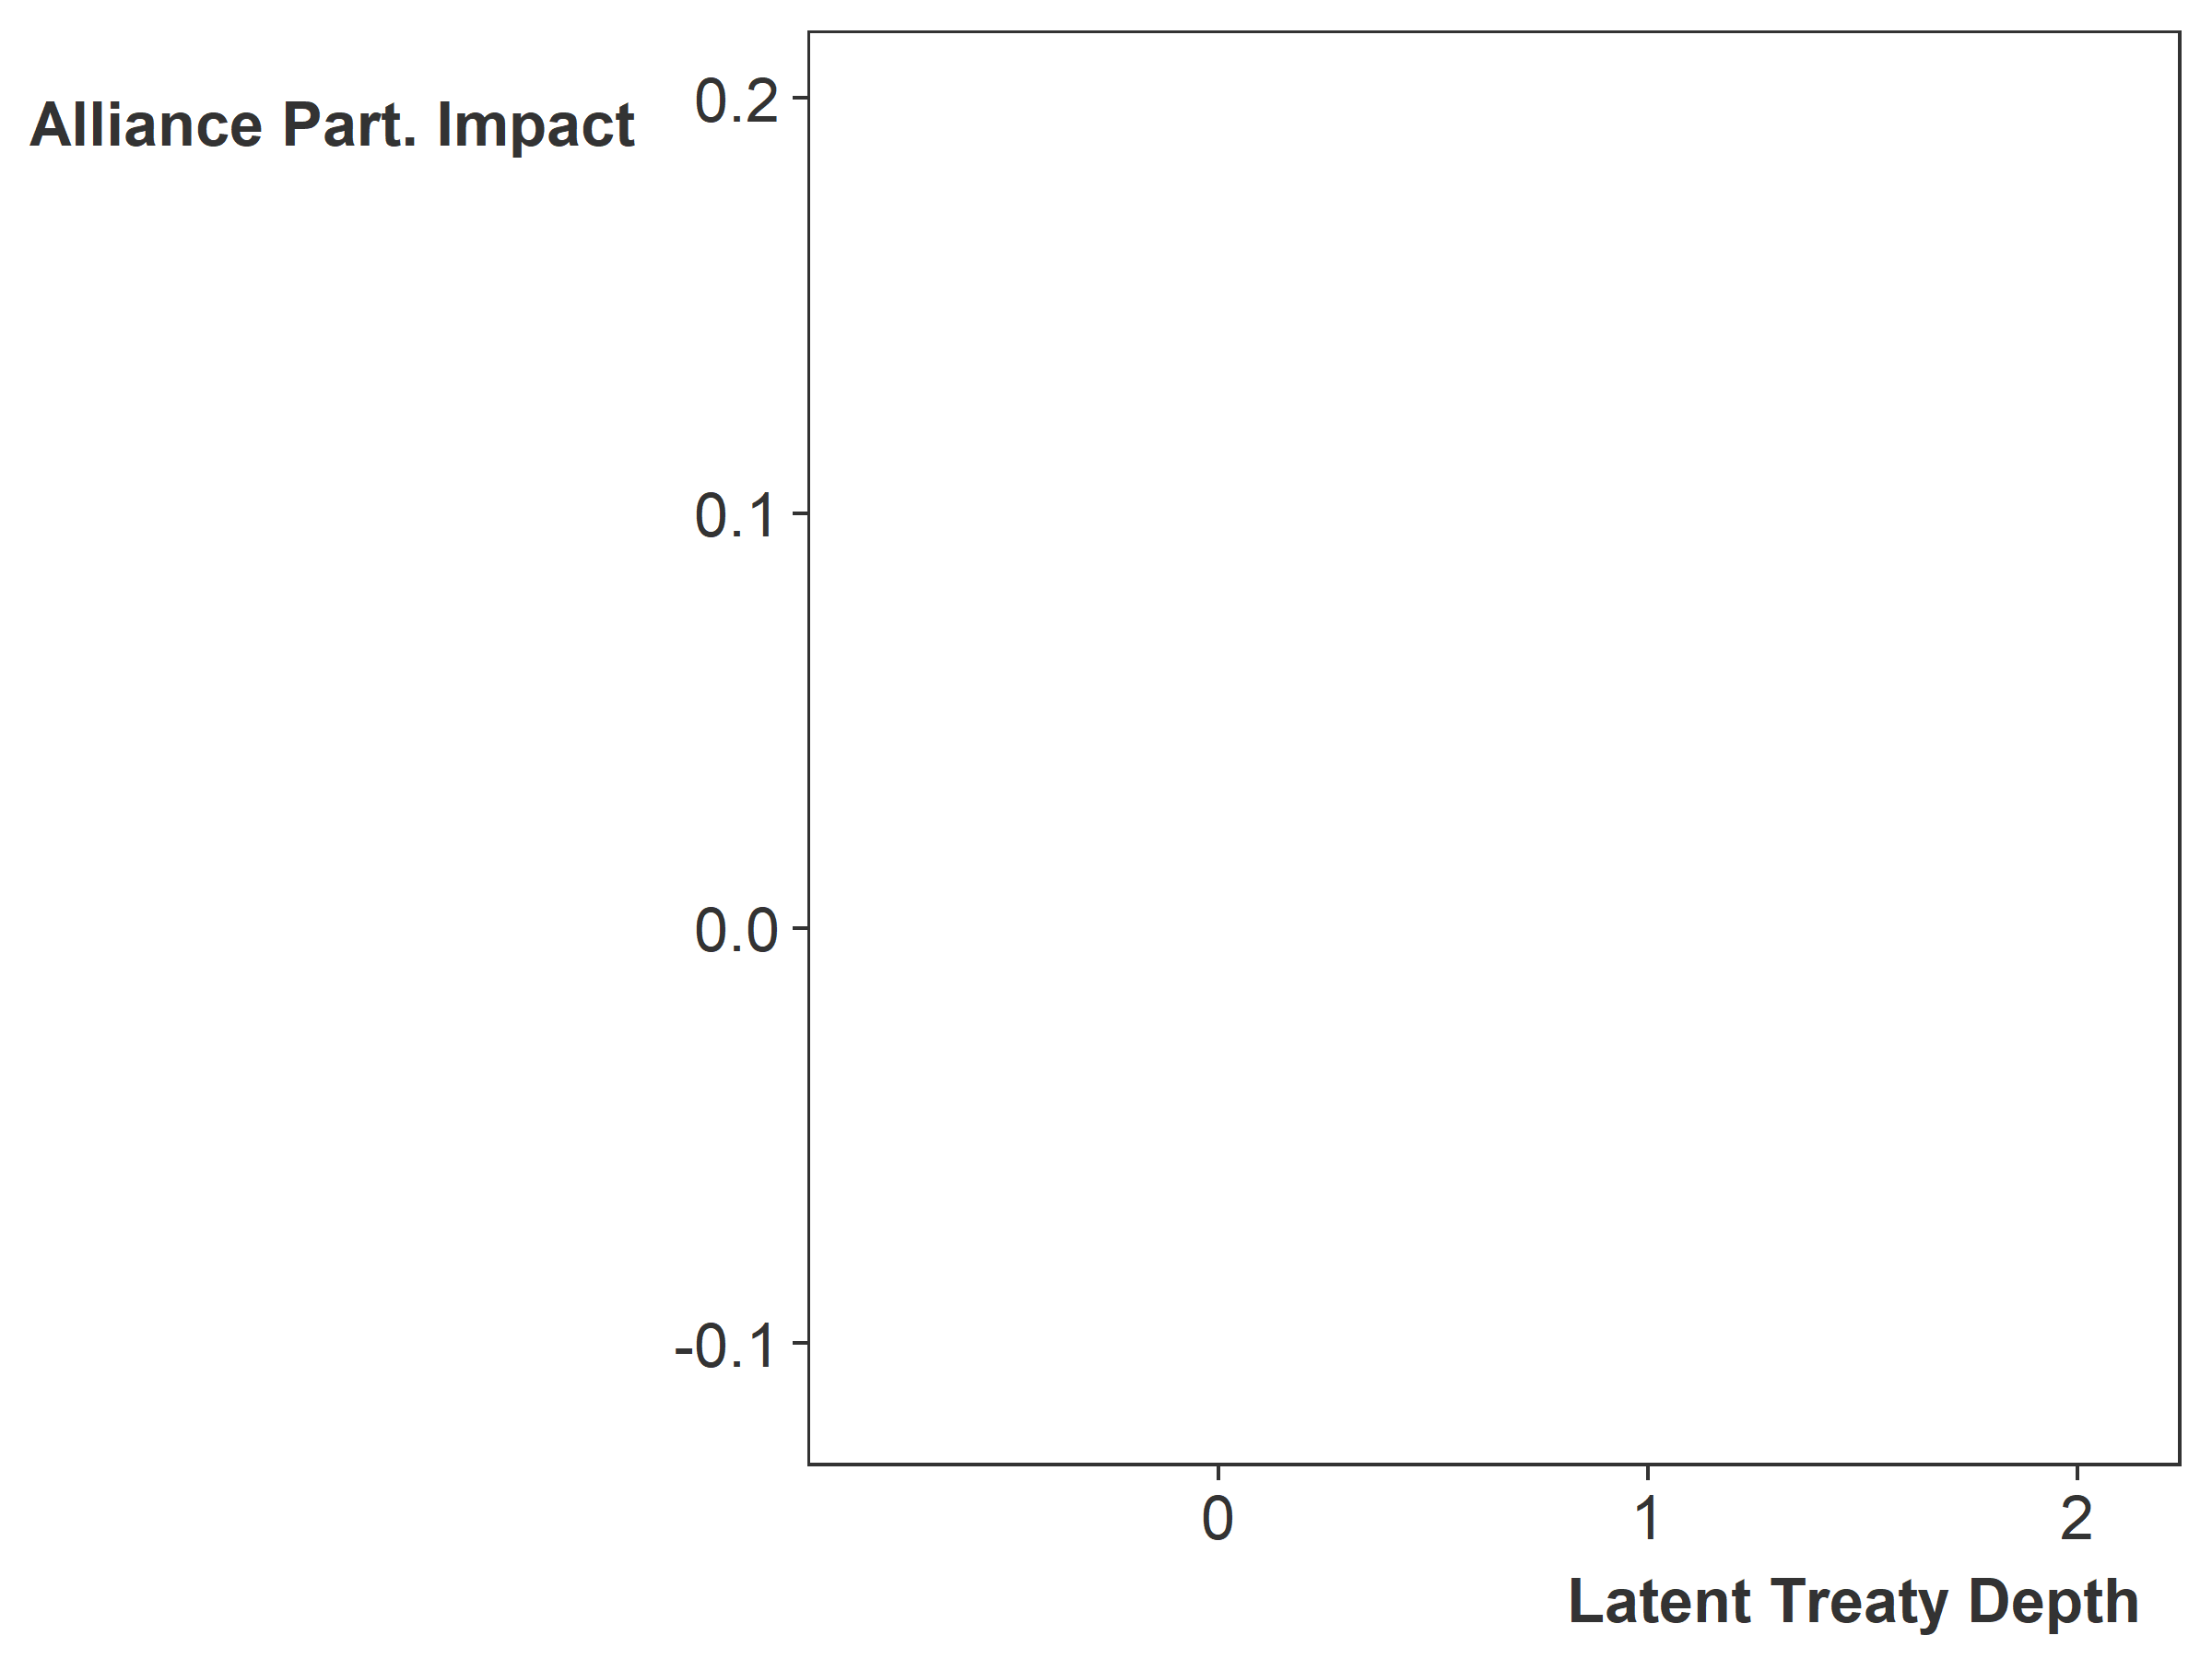
\includegraphics[width=0.95\textwidth]{ld-lambda-blank.png}
	\label{fig:ld-lambda-blank}
\end{figure}


\end{frame}


%------------------------------------------------

\begin{frame}{Treaty Depth and Alliance Coefficients}

\begin{figure}
	\centering
		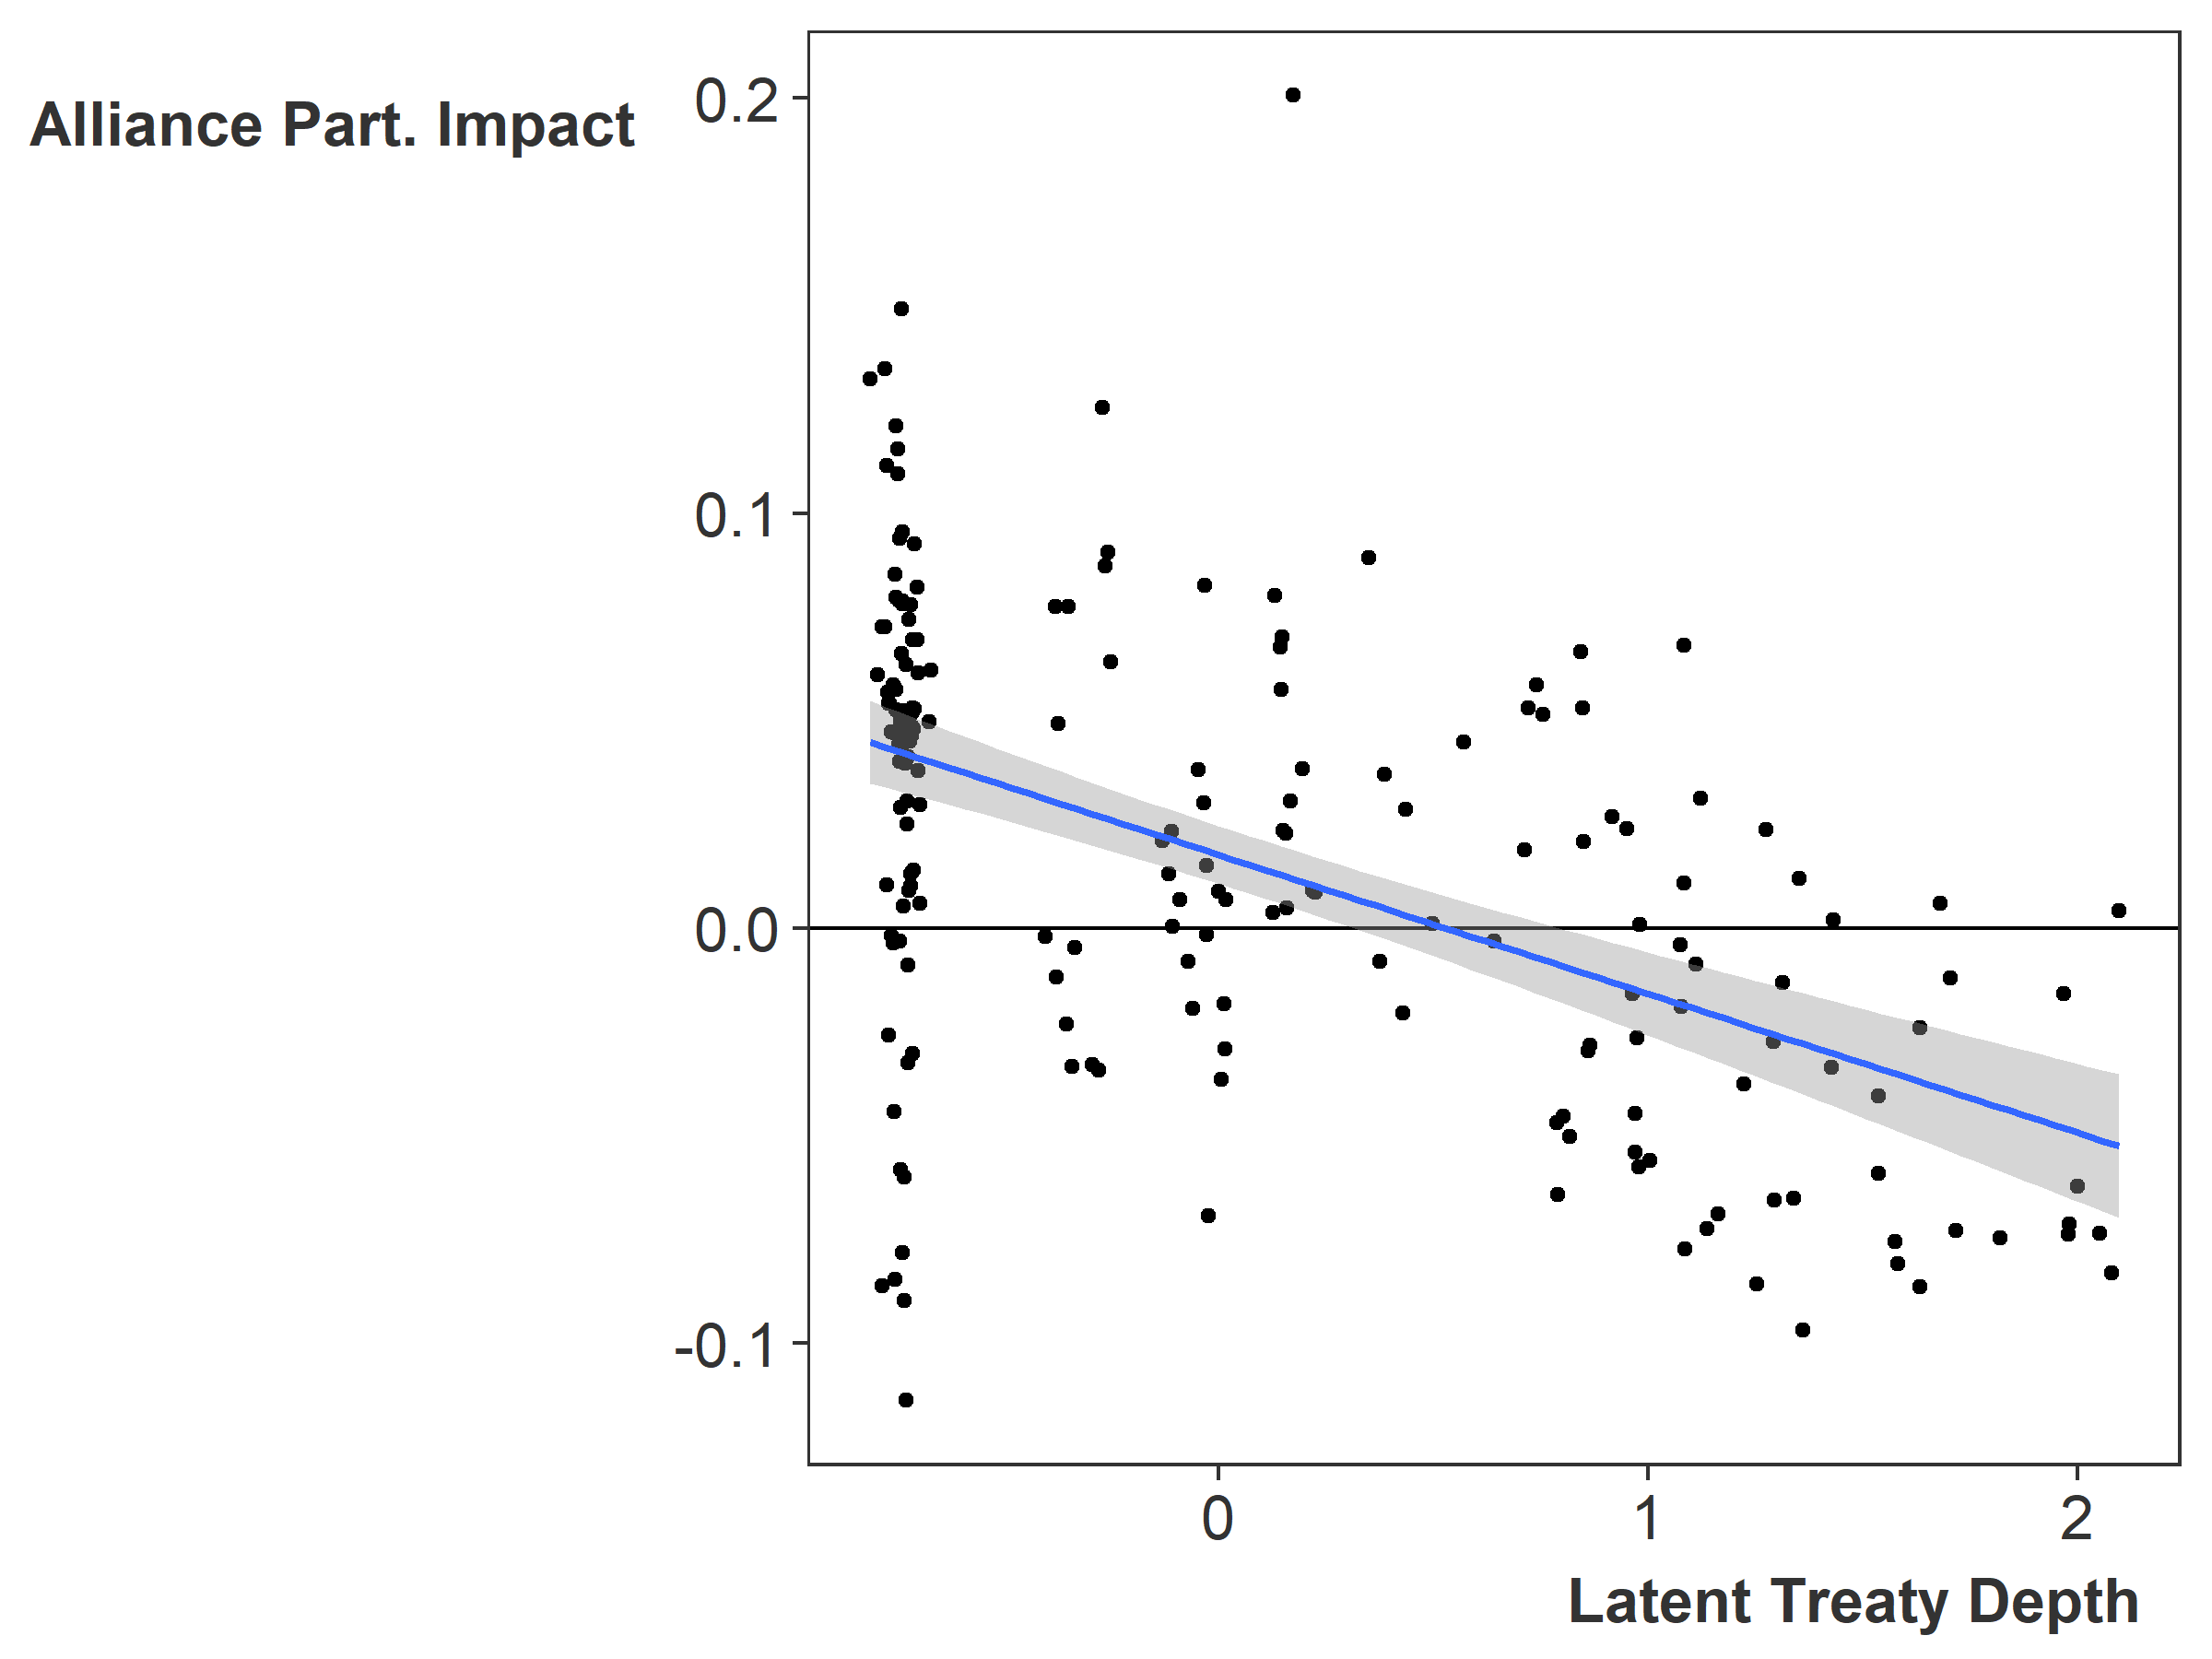
\includegraphics[width=0.9\textwidth]{ld-lambda-min.png}
	\label{fig:ld-lambda-min}
\end{figure}


\end{frame}

%------------------------------------------------

\begin{frame}{Predicted Military Spending Changes}

\begin{figure}
	\centering
		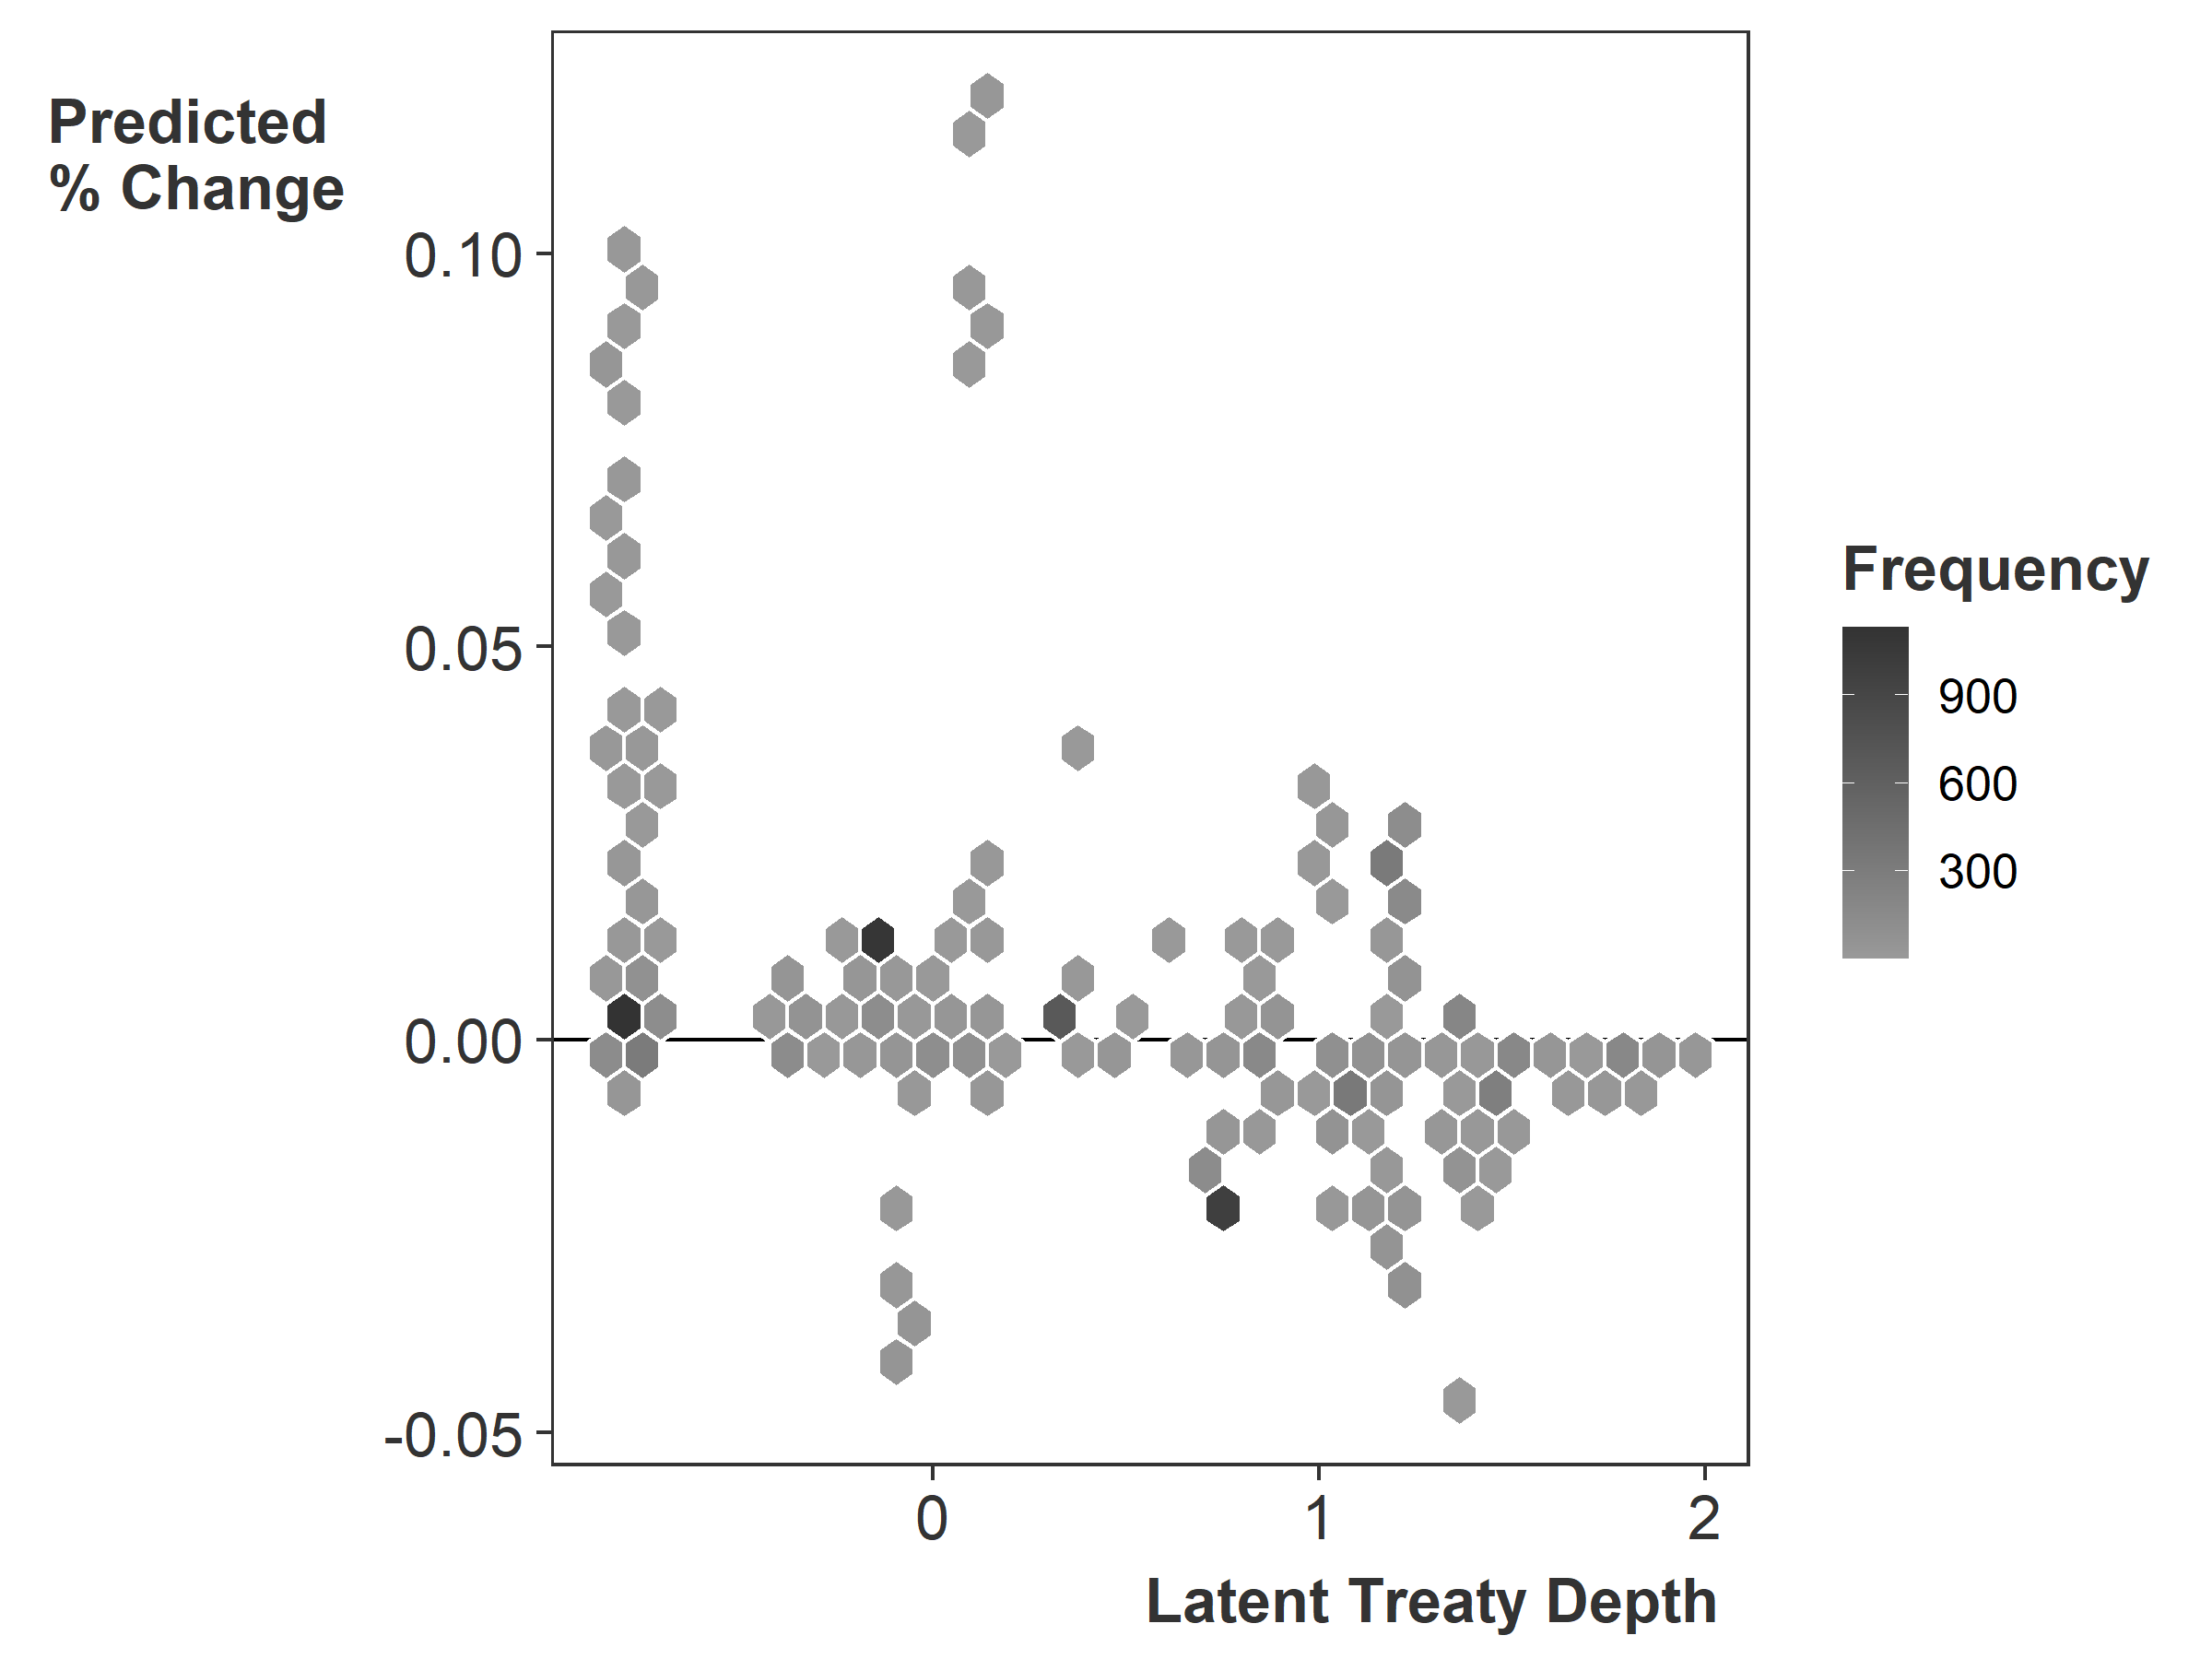
\includegraphics[width=0.9\textwidth]{ld-growth-min.png}
\end{figure}


\end{frame}

%------------------------------------------------

\section{US Alliances}

%------------------------------------------------

\begin{frame}{Reassurance}

\begin{figure}
	\centering
		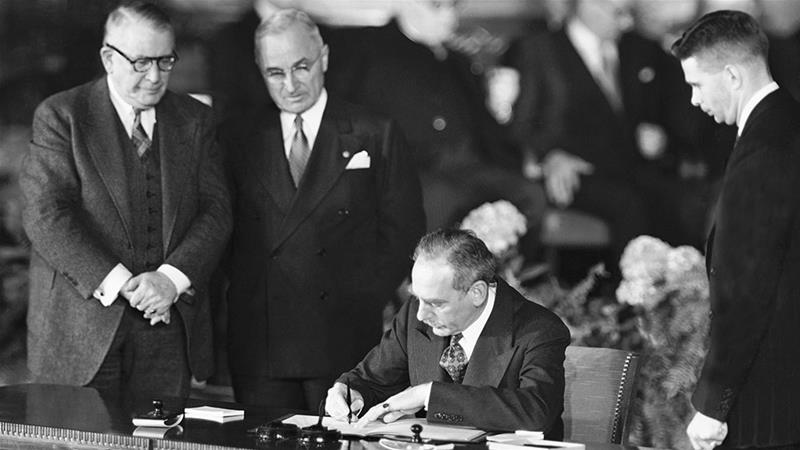
\includegraphics[width=0.95\textwidth]{acheson-nato-sign.jpg}
	\label{fig:acheson-nato-sign}
\end{figure}


\end{frame}



%------------------------------------------------

\begin{frame}{US Alliances in Context} 

\begin{figure}
	\centering
		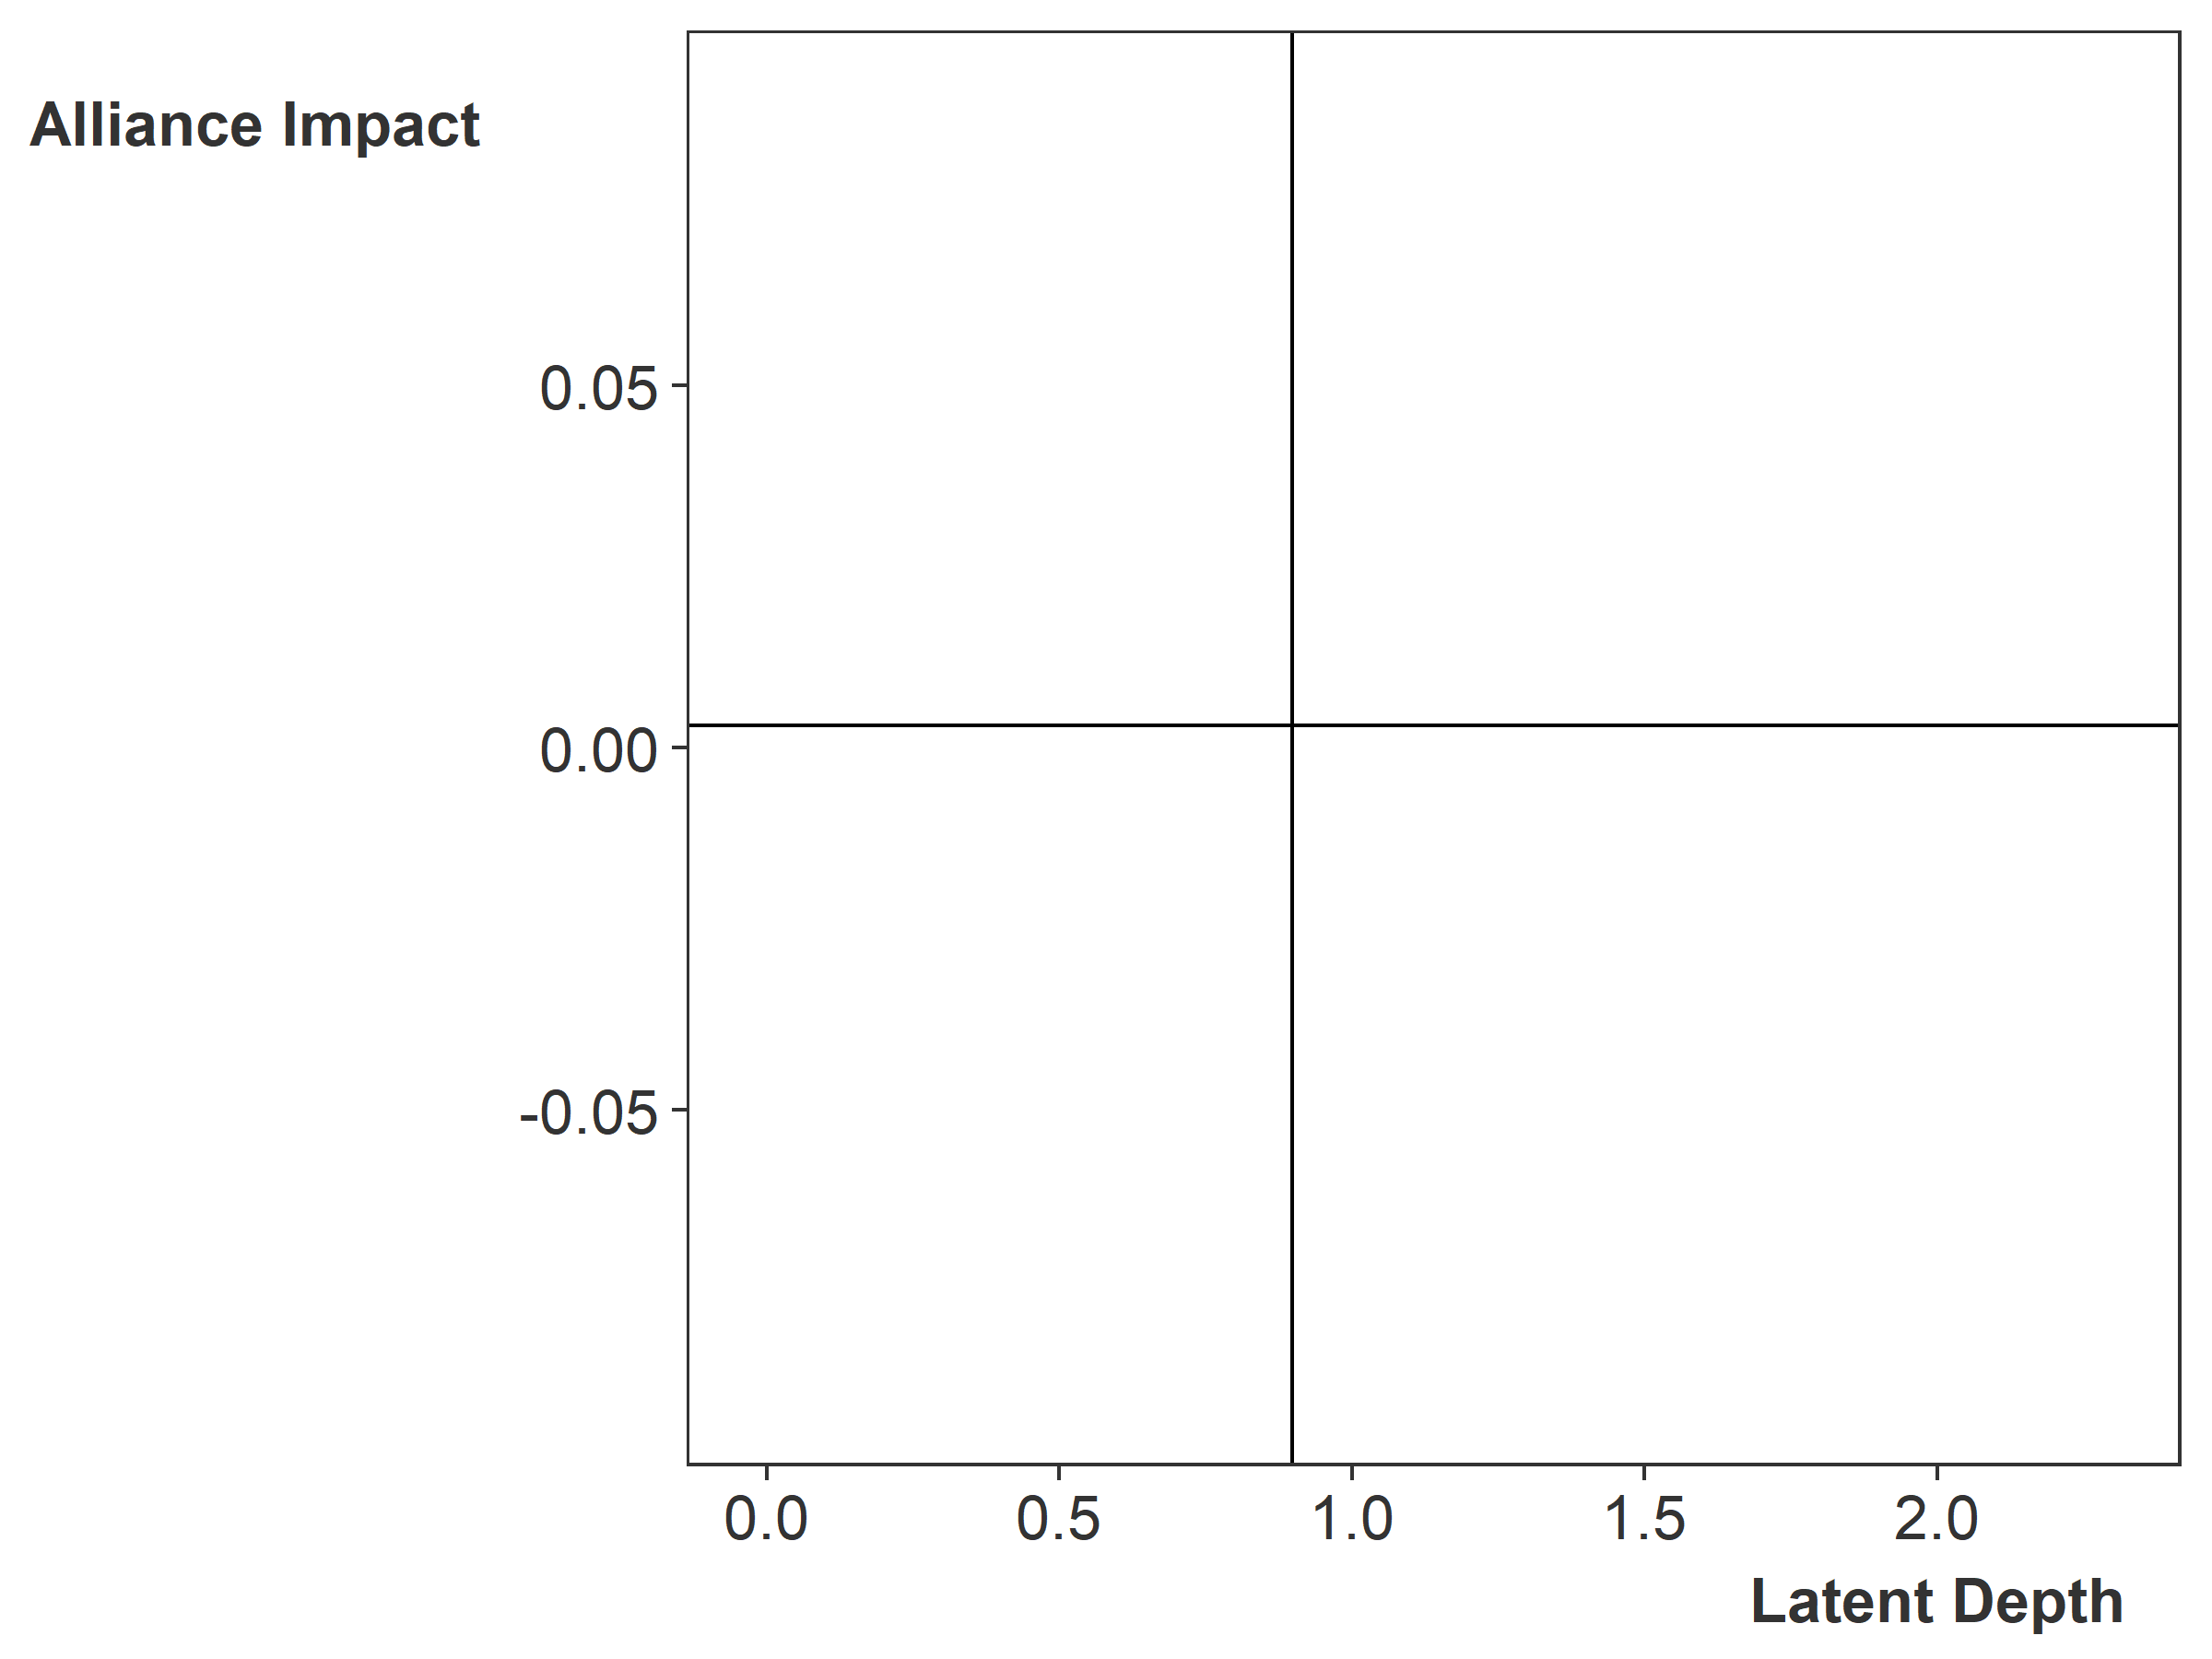
\includegraphics[width=0.95\textwidth]{lambda-depth-us-blank.png}
\end{figure}


 \end{frame}
 
 
%------------------------------------------------

\begin{frame}{US Alliances in Context} 

\begin{figure}
	\centering
		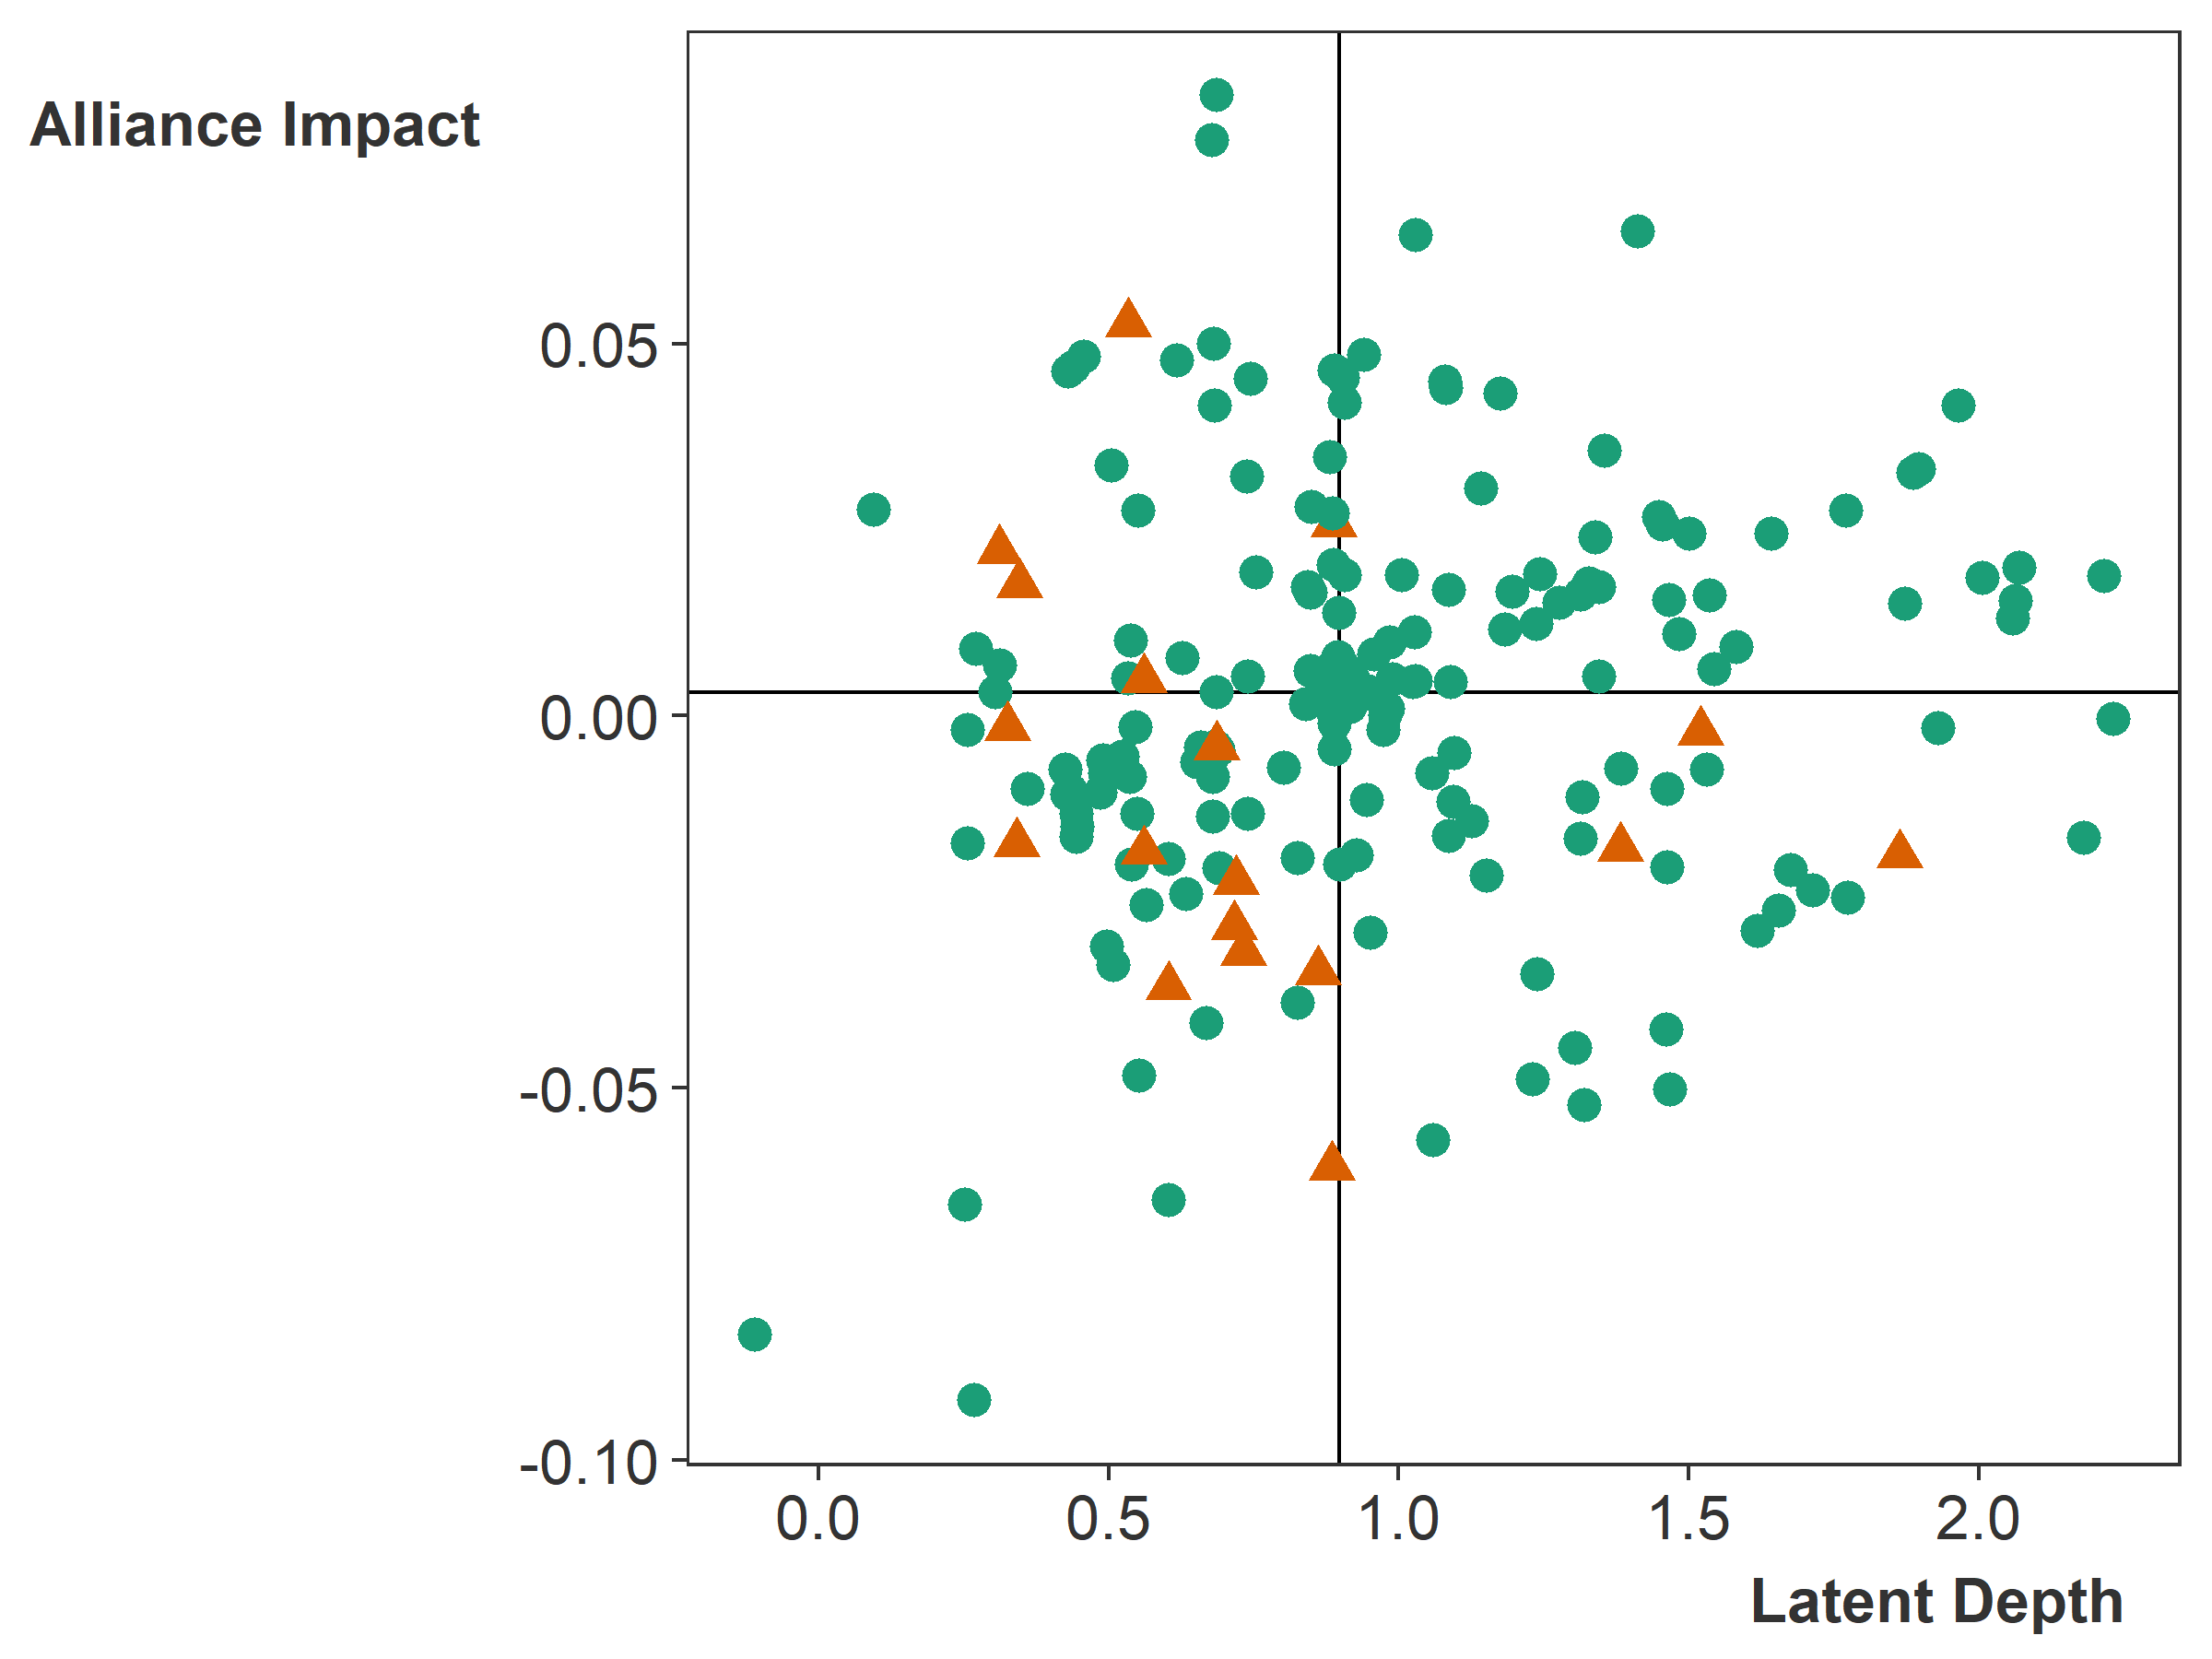
\includegraphics[width=0.95\textwidth]{lambda-depth-us.png}
\end{figure}


 \end{frame}



%-----------------------------------------------

\begin{frame}{Implication: What to do with US alliances?}

\begin{figure}[htbp]
	\centering
		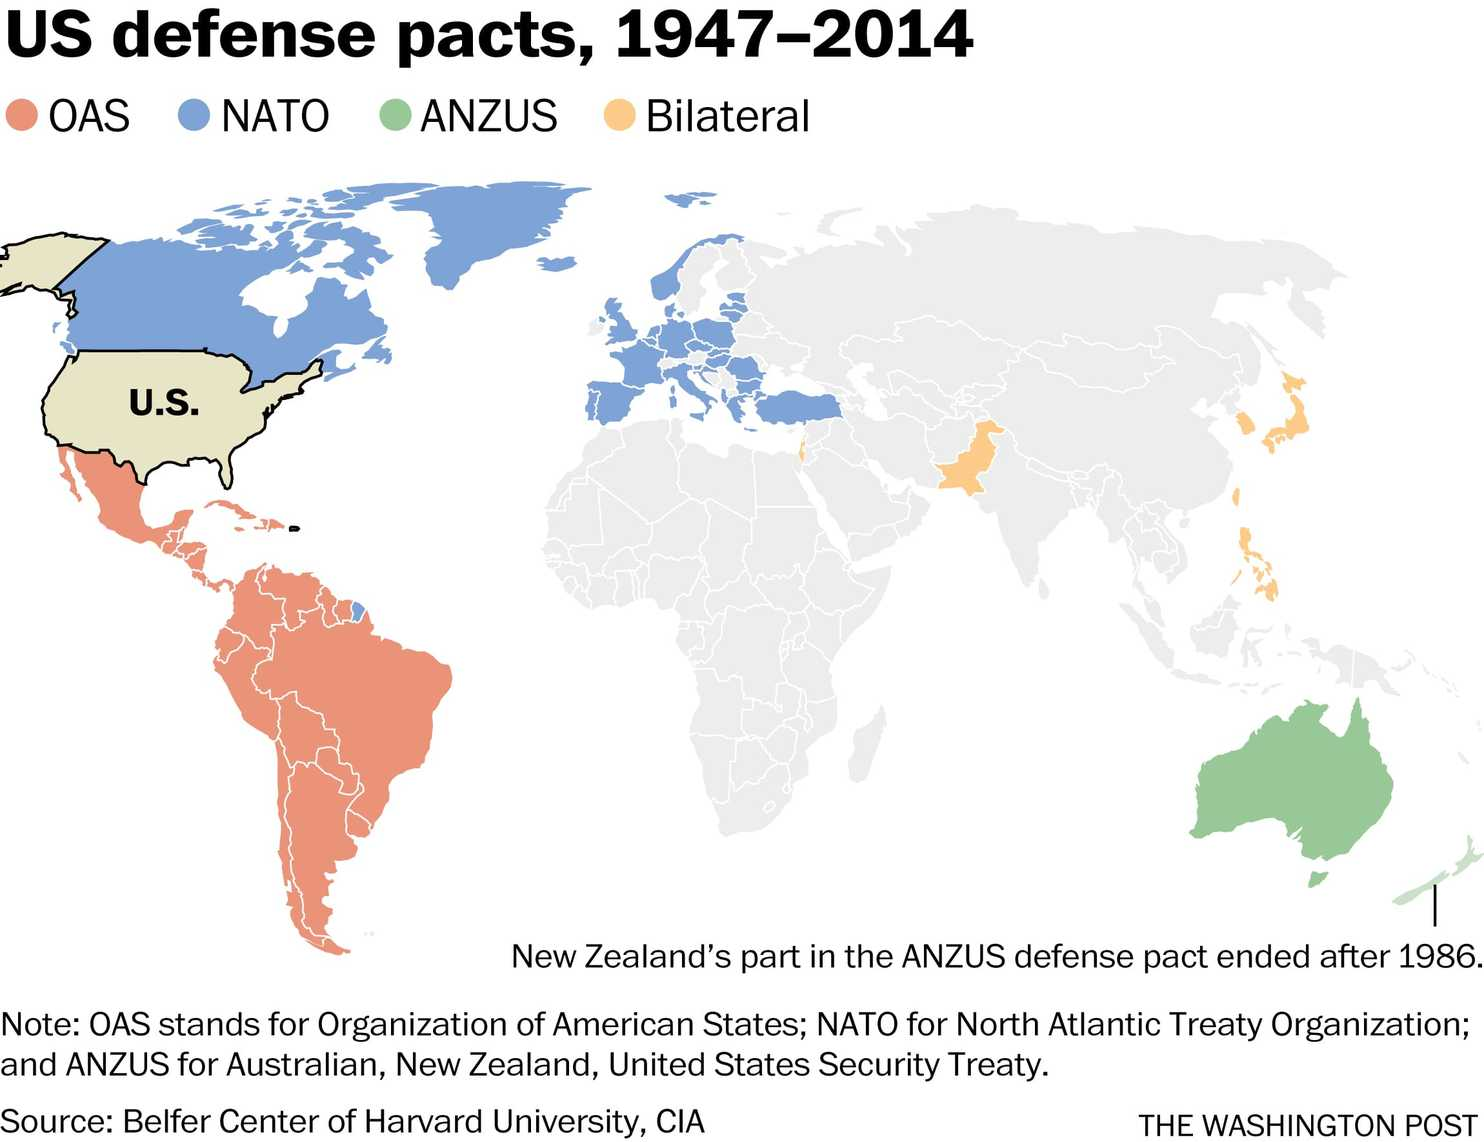
\includegraphics[width=0.95\textwidth]{nato-map.jpg}
\end{figure}


\end{frame}


%-----------------------------------------------

\section{Conclusion}

%-----------------------------------------------

\begin{frame}[standout]

How alliance participation affects military spending depends on treaty depth.  

\end{frame}

%------------------------------------------------
% The two subpoints 
 \begin{frame}[standout]

Deep alliances often reduce non-major power military spending but shallow alliances often increase military spending. 

 \end{frame}
 
 
%------------------------------------------------
% The two subpoints 
 \begin{frame}[standout]

There is a tradeoff between reassurance and non-major power military spending in alliance treaty design. 

 \end{frame}


%-----------------------------------------------

\section{Looking Ahead}

%-----------------------------------------------


\begin{frame}{My Research Agenda: Political Economy of Security}

\begin{columns}

% Major powers
\begin{column}{0.5\textwidth}
\textbf{International Security}
\begin{enumerate} 
\item Alliance Participation and Military Spending 
\item Democracy, Electoral Competition and Alliance Treaty Depth
\item Collective Action or Exchange?: Framing Cooperation in International Alliances 
\item Reassessing the Public Goods Theory of Alliances
\end{enumerate} 
\end{column}



\begin{column}{0.5\textwidth}
\textbf{Intra-State Conflict}
\begin{enumerate}
\item Post-Civil War Conflict Management Institutions and FDI 
\item U.S. Foreign Terrorist Organization (FTO) List and Terrorist Attacks
\item International Engagement and Rebel Groups’ Commitment to International Law  (\textit{Forthcoming})
\end{enumerate} 
\end{column}

\end{columns}
 

\end{frame}


%-----------------------------------------------

 \begin{frame}[standout]

Thank you! 

jkalley@virginia.edu

 \end{frame}


%-----------------------------------------------

\appendix 


%-----------------------------------------------

\begin{frame}{Limitations}

\begin{enumerate}
\item Domestic political economy of military spending. 
\item Measurement error and missing data. 
\item Formal depth only in the measure. 
\item Strategic alliance design. 
\end{enumerate}

\end{frame}

%-----------------------------------------------

\begin{frame}{Sources of Alliance Treaty Depth}

Democracy, specifically electoral competition, encourages deep alliances. 
\begin{enumerate}
\item Depth adds credibility, but the costs are not very transparent. 
\item Harder for opposition politicians to critique than unconditional support.  
\end{enumerate}

\end{frame}


%----------------------------------------------

\begin{frame}{Leeds and Anac 2005 Performance Analysis}

\begin{table}[!htbp] \centering 
\begin{adjustbox}{width= .95\textwidth, center}
\begin{tabular}{@{\extracolsep{5pt}}lccc} 
\\[-1.8ex]\hline 
\hline \\[-1.8ex] 
 & \multicolumn{3}{c}{\textit{Dependent variable:}} \\ 
\cline{2-4} 
\\[-1.8ex] & \multicolumn{2}{c}{Leeds and Anac} & Berkemeier and Fuhrmann \\ 
\\[-1.8ex] & (1) & (2) & (3)\\ 
\hline \\[-1.8ex] 
 Military Institutionalization & $-$0.543 &  &  \\ 
  & ($-$1.306, 0.221) &  &  \\ 
  Latent Depth &  & 0.173 & 0.373 \\ 
  &  & ($-$0.583, 0.929) & ($-$0.384, 1.131) \\ 
  Alliance Formality & $-$1.161$^{}$ & $-$1.512$^{}$ &  \\ 
  & ($-$2.082, $-$0.240) & ($-$2.466, $-$0.558) &  \\ 
  Capability Change & $-$1.841$^{}$ & $-$1.928$^{}$ &  \\ 
  & ($-$3.135, $-$0.547) & ($-$3.251, $-$0.604) &  \\ 
  Process Change & $-$1.802$^{}$ & $-$1.462$^{}$ &  \\ 
  & ($-$3.336, $-$0.269) & ($-$2.886, $-$0.039) &  \\ 
  Original Target & $-$0.723 & $-$0.788 &  \\ 
  & ($-$1.849, 0.403) & ($-$1.942, 0.366) &  \\ 
\hline \\[-1.8ex] 
\textit{Note:}  & \multicolumn{3}{r}{95\% Confidence Intervals in Parentheses. Controls in Model 3 ommitted.} \\ 
\end{tabular}
\end{adjustbox} 
\end{table}


\end{frame}


%------------------------------------------------

\begin{frame}{Details of Measurement Model}

\begin{itemize}
\item Bayesian Gaussian Copula Factor Model: for mixed data. 
\item Uses copulas to break dependence between latent factors and marginal distributions. 
\item Treats marginals as unknown and keeps them free of dependence. 
\item IMH proposal, 10,000 iteration warmup, 20,000 samples, thinned every 20 draws. 
\item Generalized double Pareto prior for the factor loading--- flexible generalized Laplace distribution with a spike at zero and heavy tails. 
\end{itemize} 


\end{frame}


%------------------------------------------------


\begin{frame}{Alternative Measure: Benson and Clinton 2016}

\begin{itemize}
\item Use a measurement model to infer alliance scope, depth and capability. 
\item Identify three separate dimensions, and use three models- explicit constraint. 
\item Their depth measure includes issue linkages.  
\item Murray et al's model relaxes distributional assumptions in their estimator (Quinn 2004 Factor Analysis). 
\end{itemize}


\end{frame}

%------------------------------------------------

\begin{frame}{Factors Comparison}

\begin{figure}
	\centering
		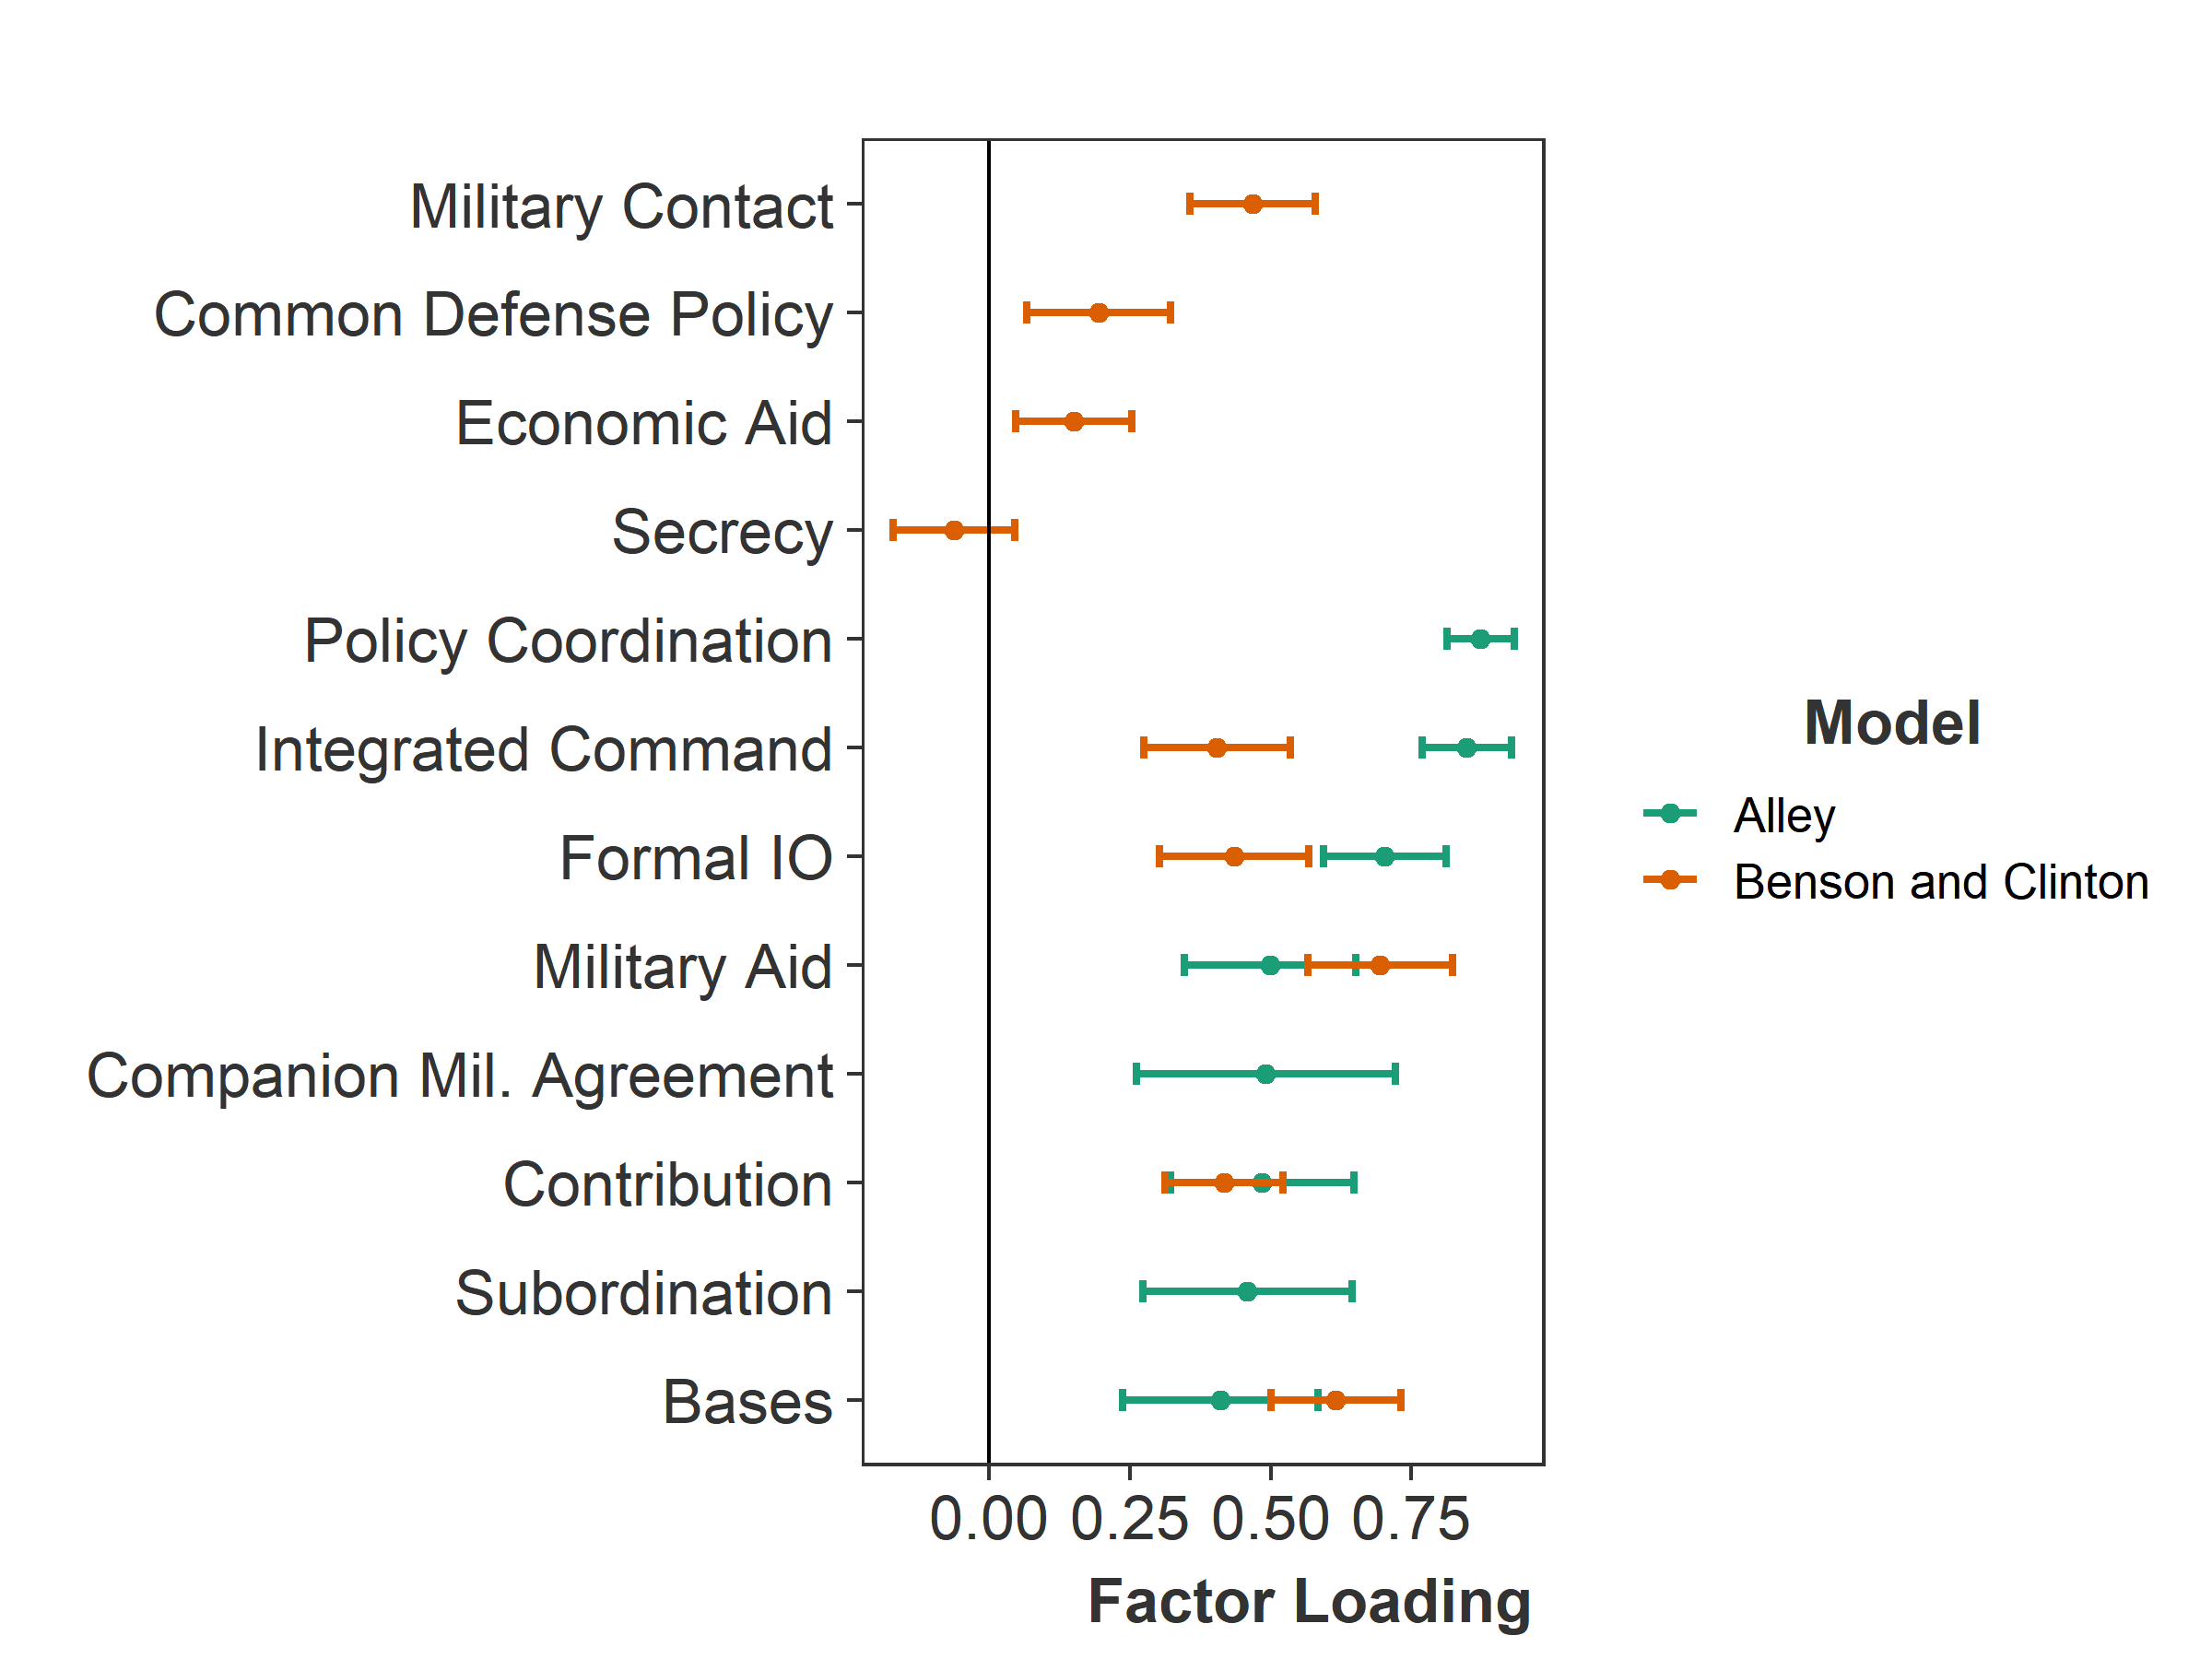
\includegraphics[width=0.95\textwidth]{bc-factor-comp.png}
\end{figure}

\end{frame}

%------------------------------------------------

\begin{frame}{Latent Score Comparison}

\begin{figure}
	\centering
		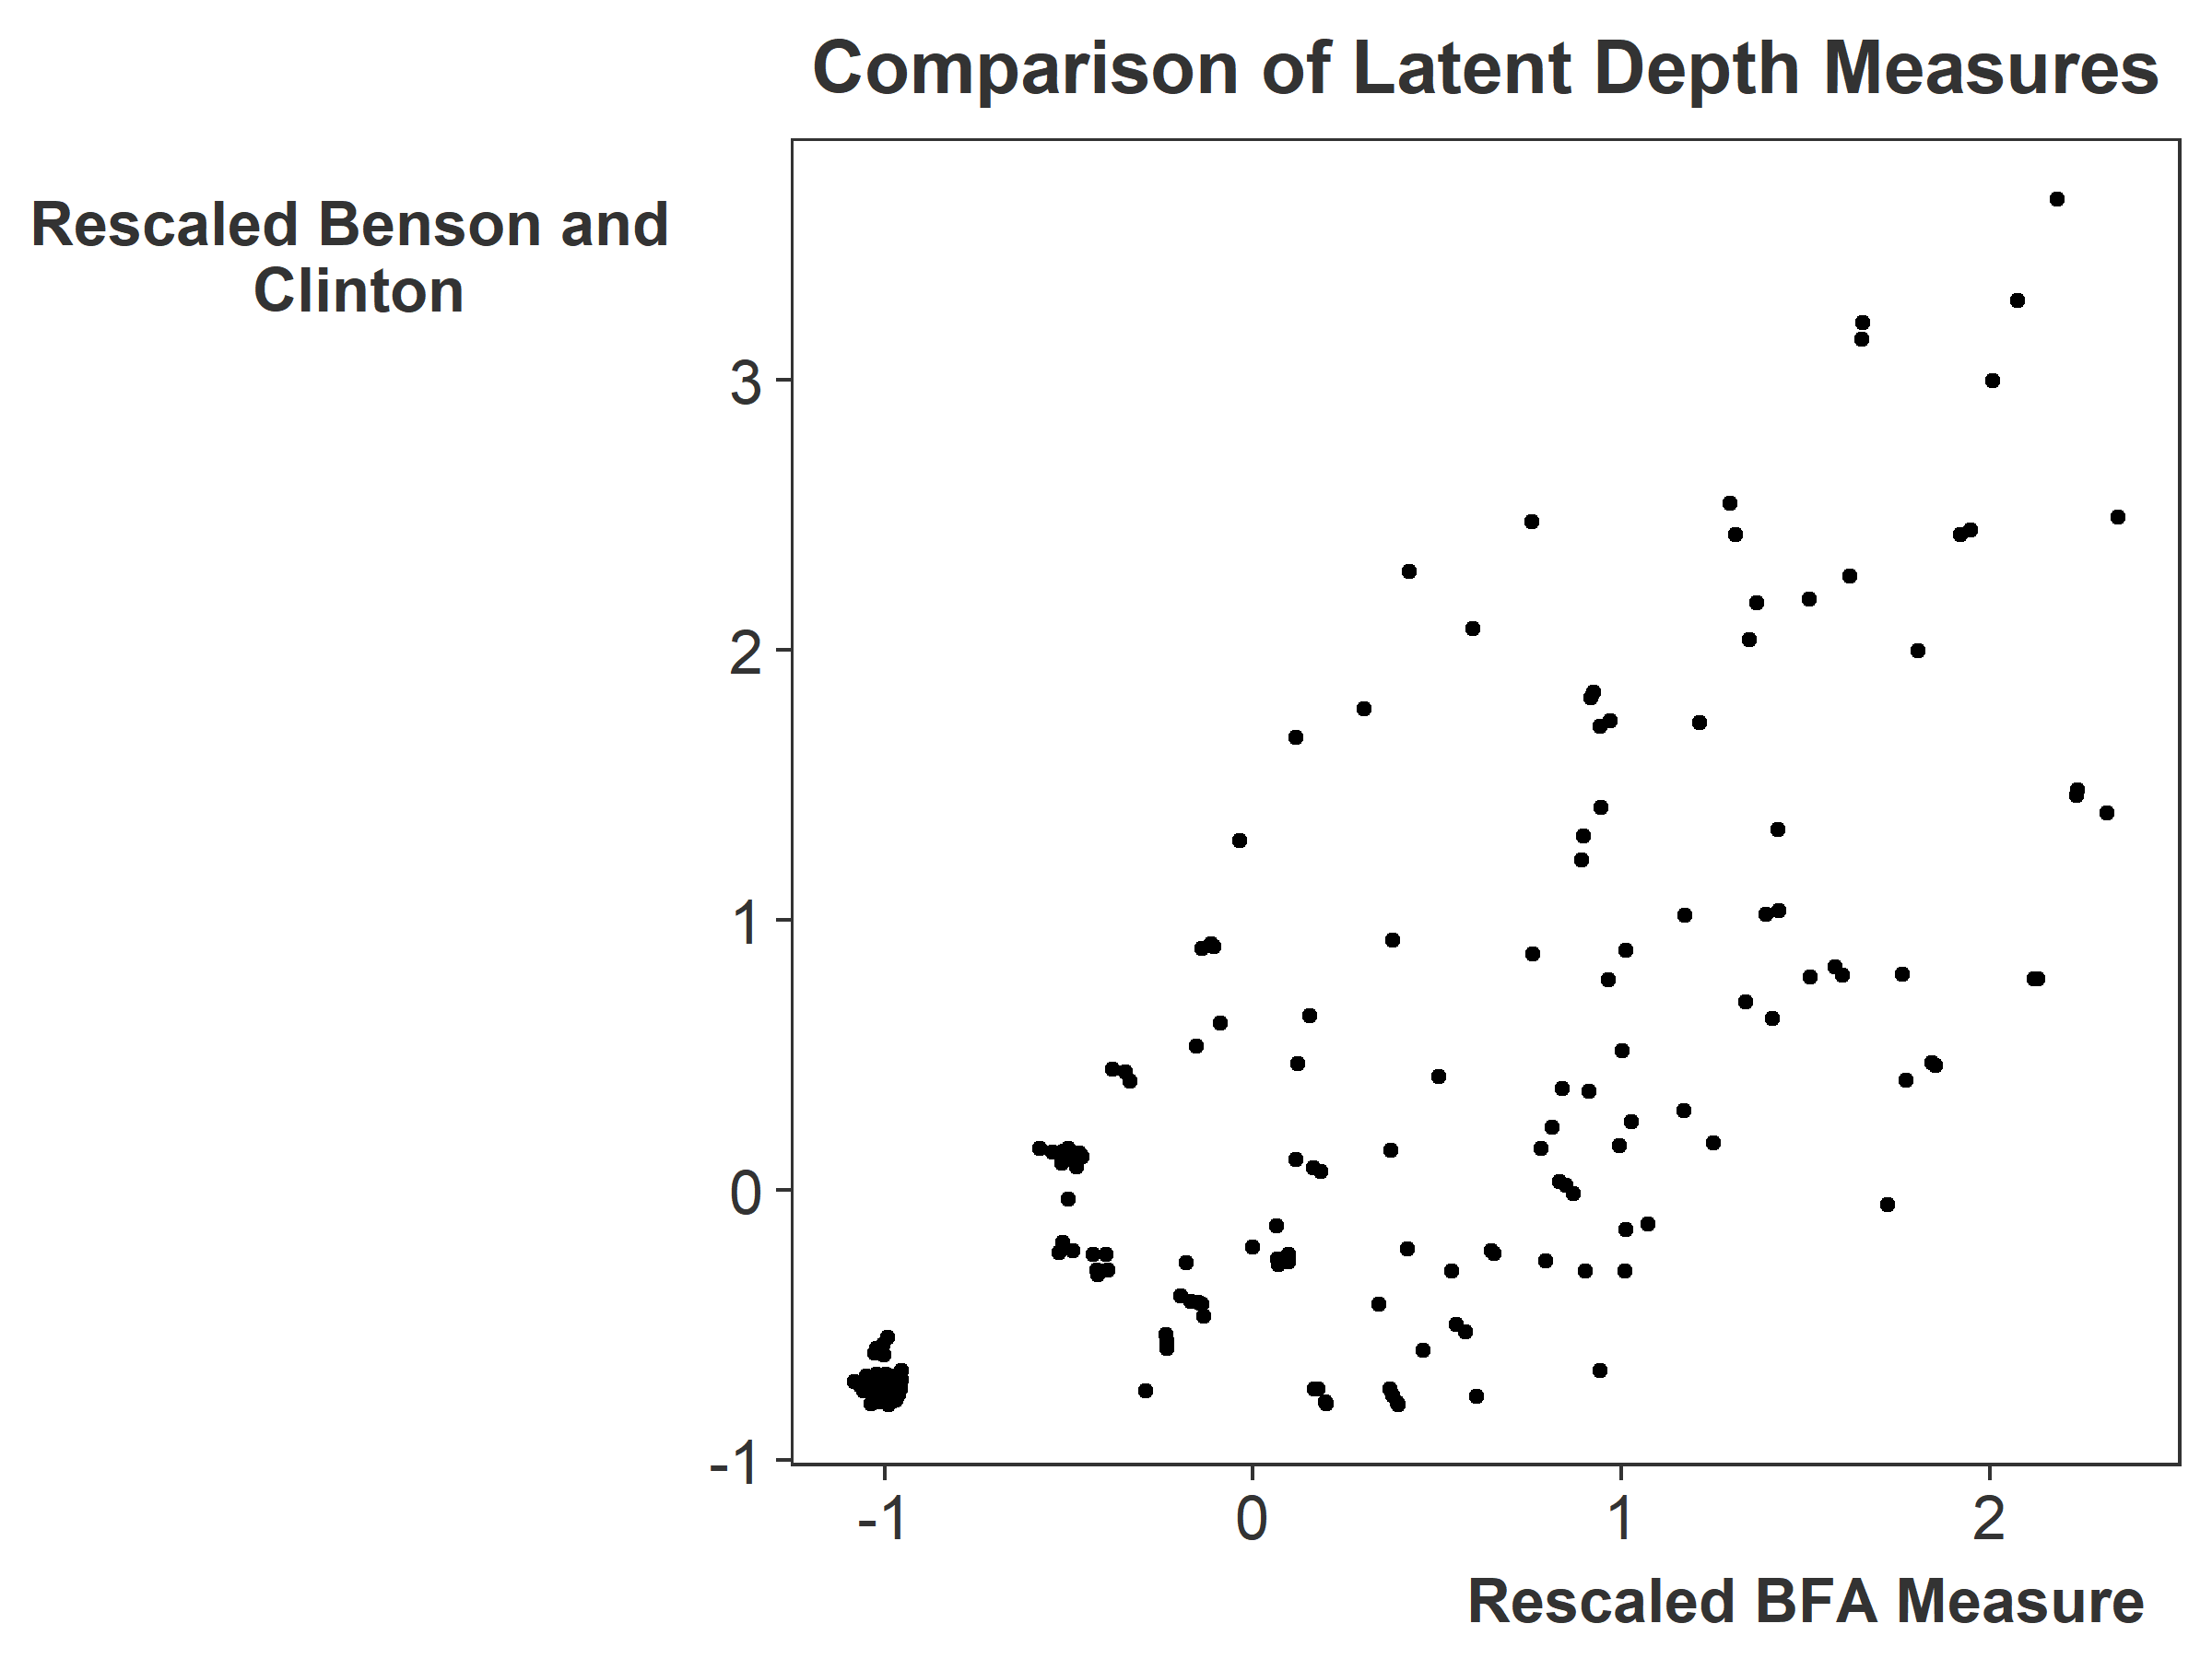
\includegraphics[width=0.95\textwidth]{bc-score-comp.png}
\end{figure}

\end{frame}


%------------------------------------------------


\begin{frame}{Alternative Measure \#2: Leeds and Anac 2005}

Ordinal measure of alliance institutionalization. 

\begin{figure}
	\centering
		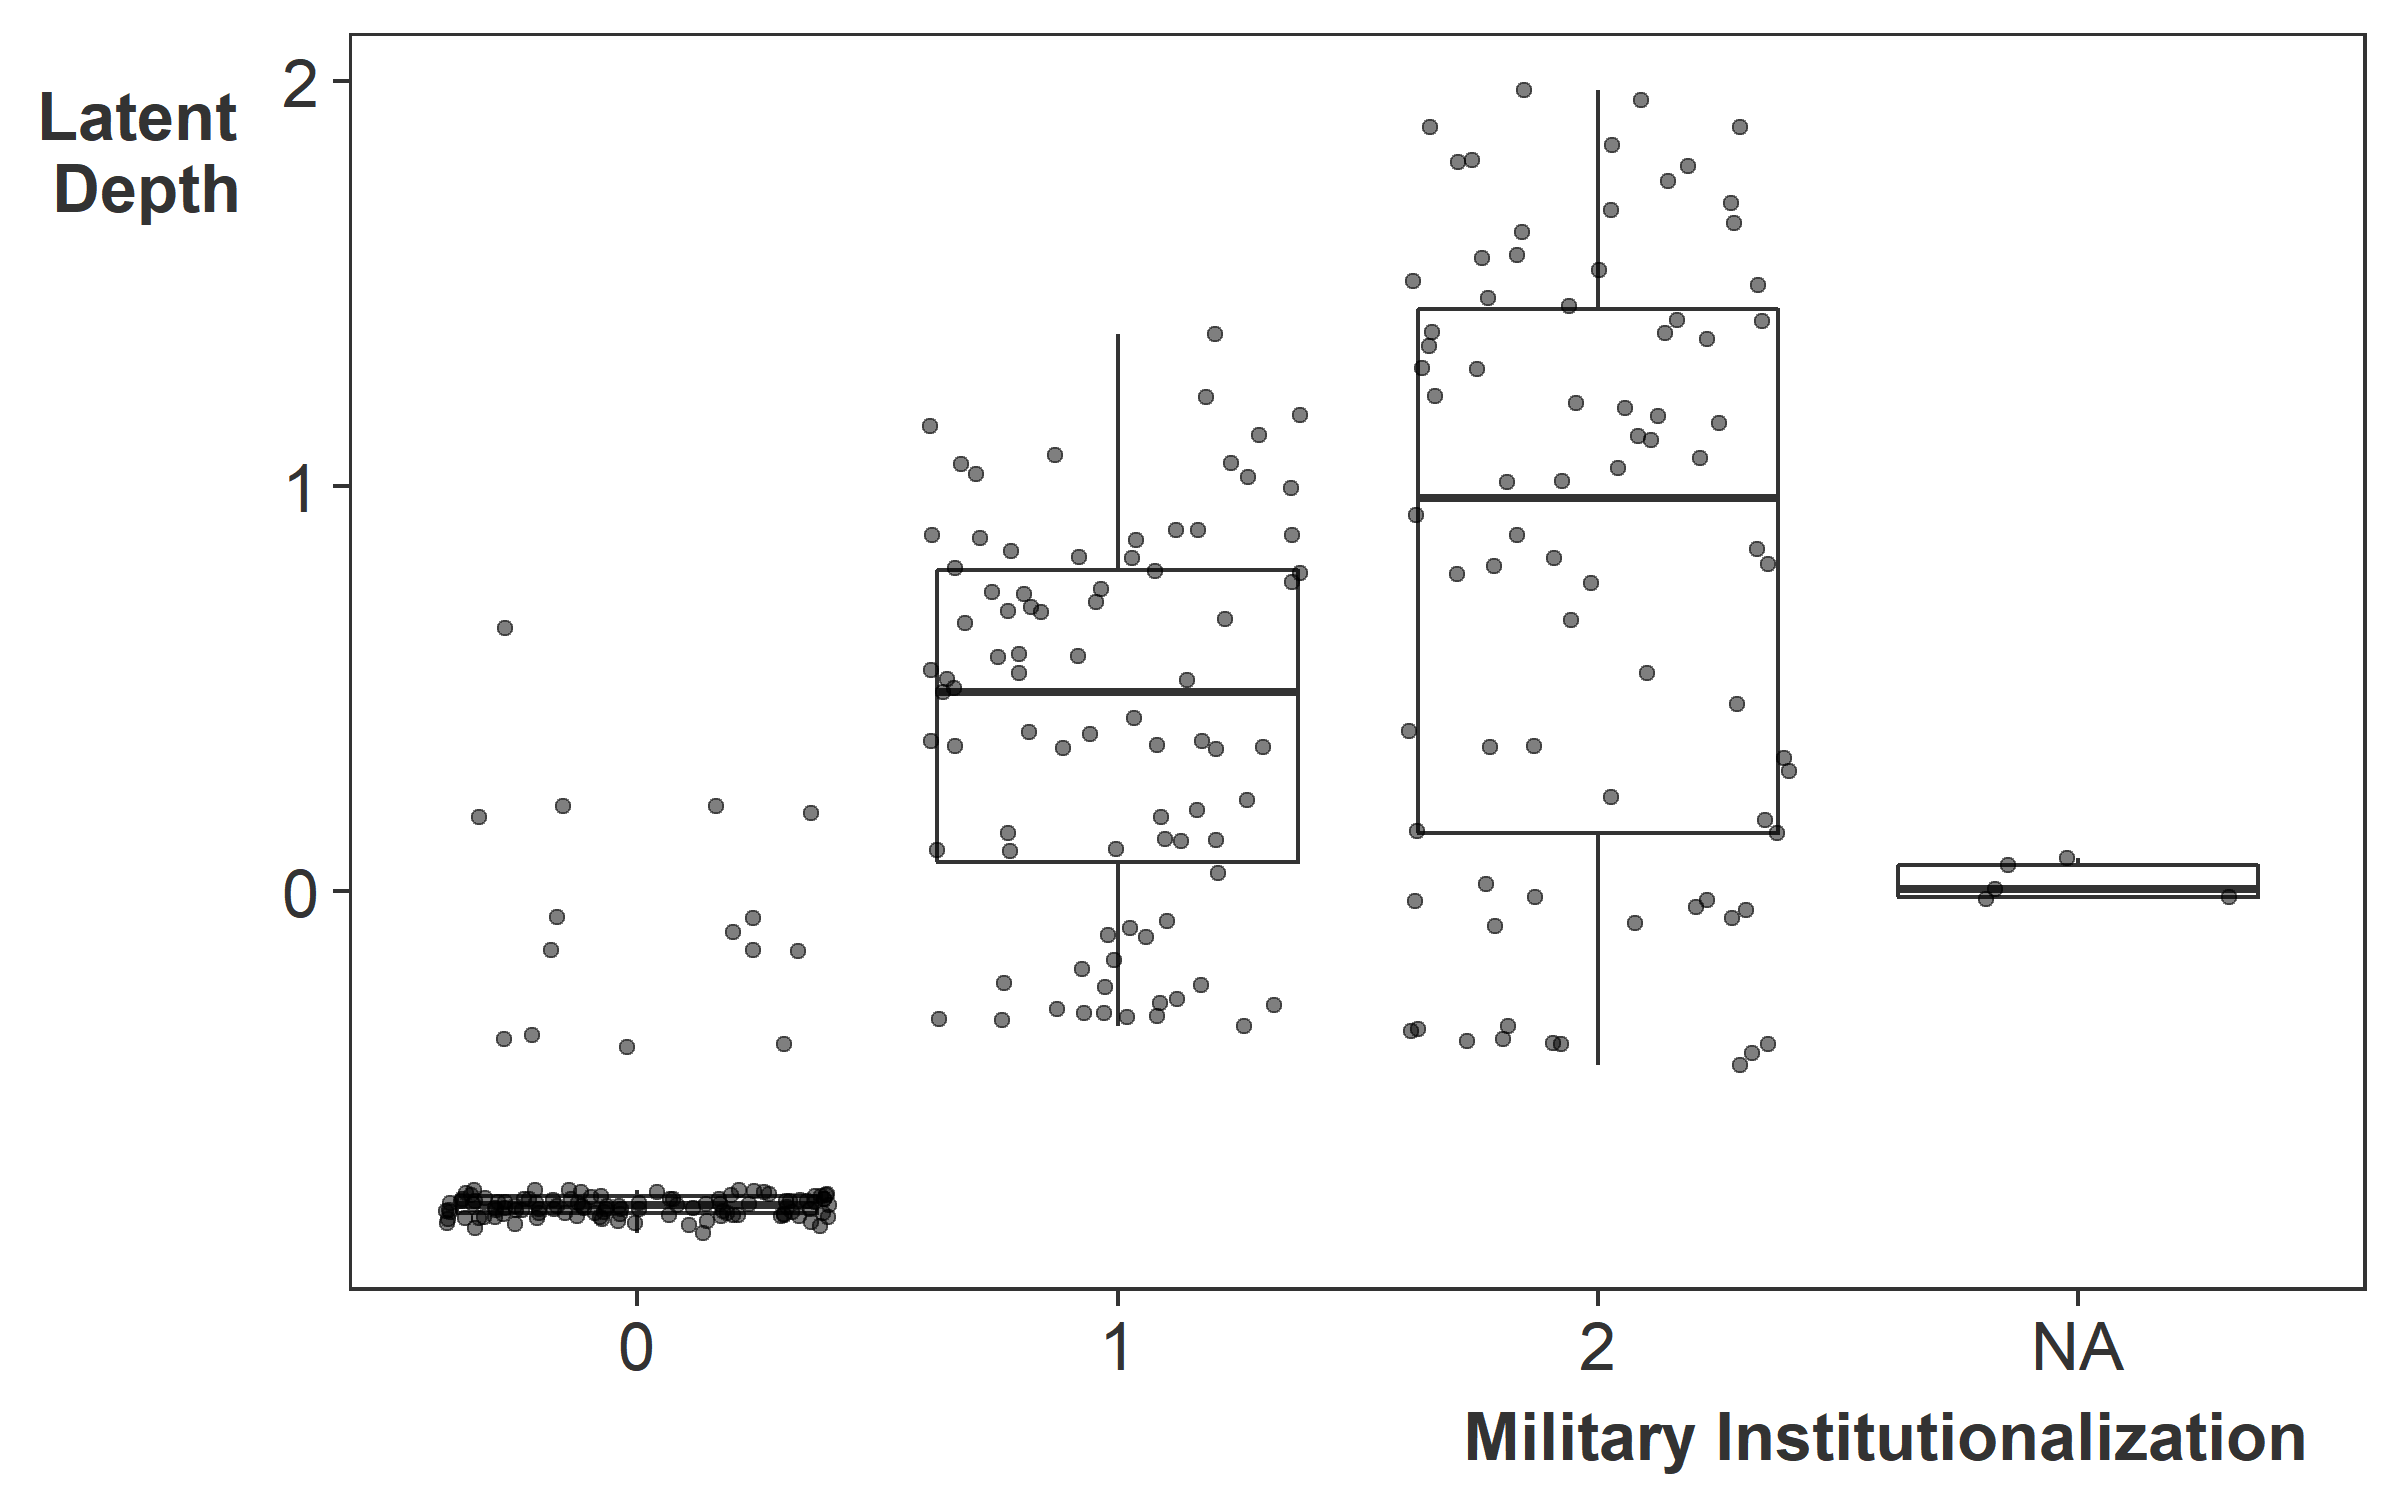
\includegraphics[width=0.95\textwidth]{milinst-comp.png}
\end{figure}


\end{frame}

%------------------------------------------------


\begin{frame}{Leeds and Anac Ordinal Measure Results}

\begin{figure}
	\centering
		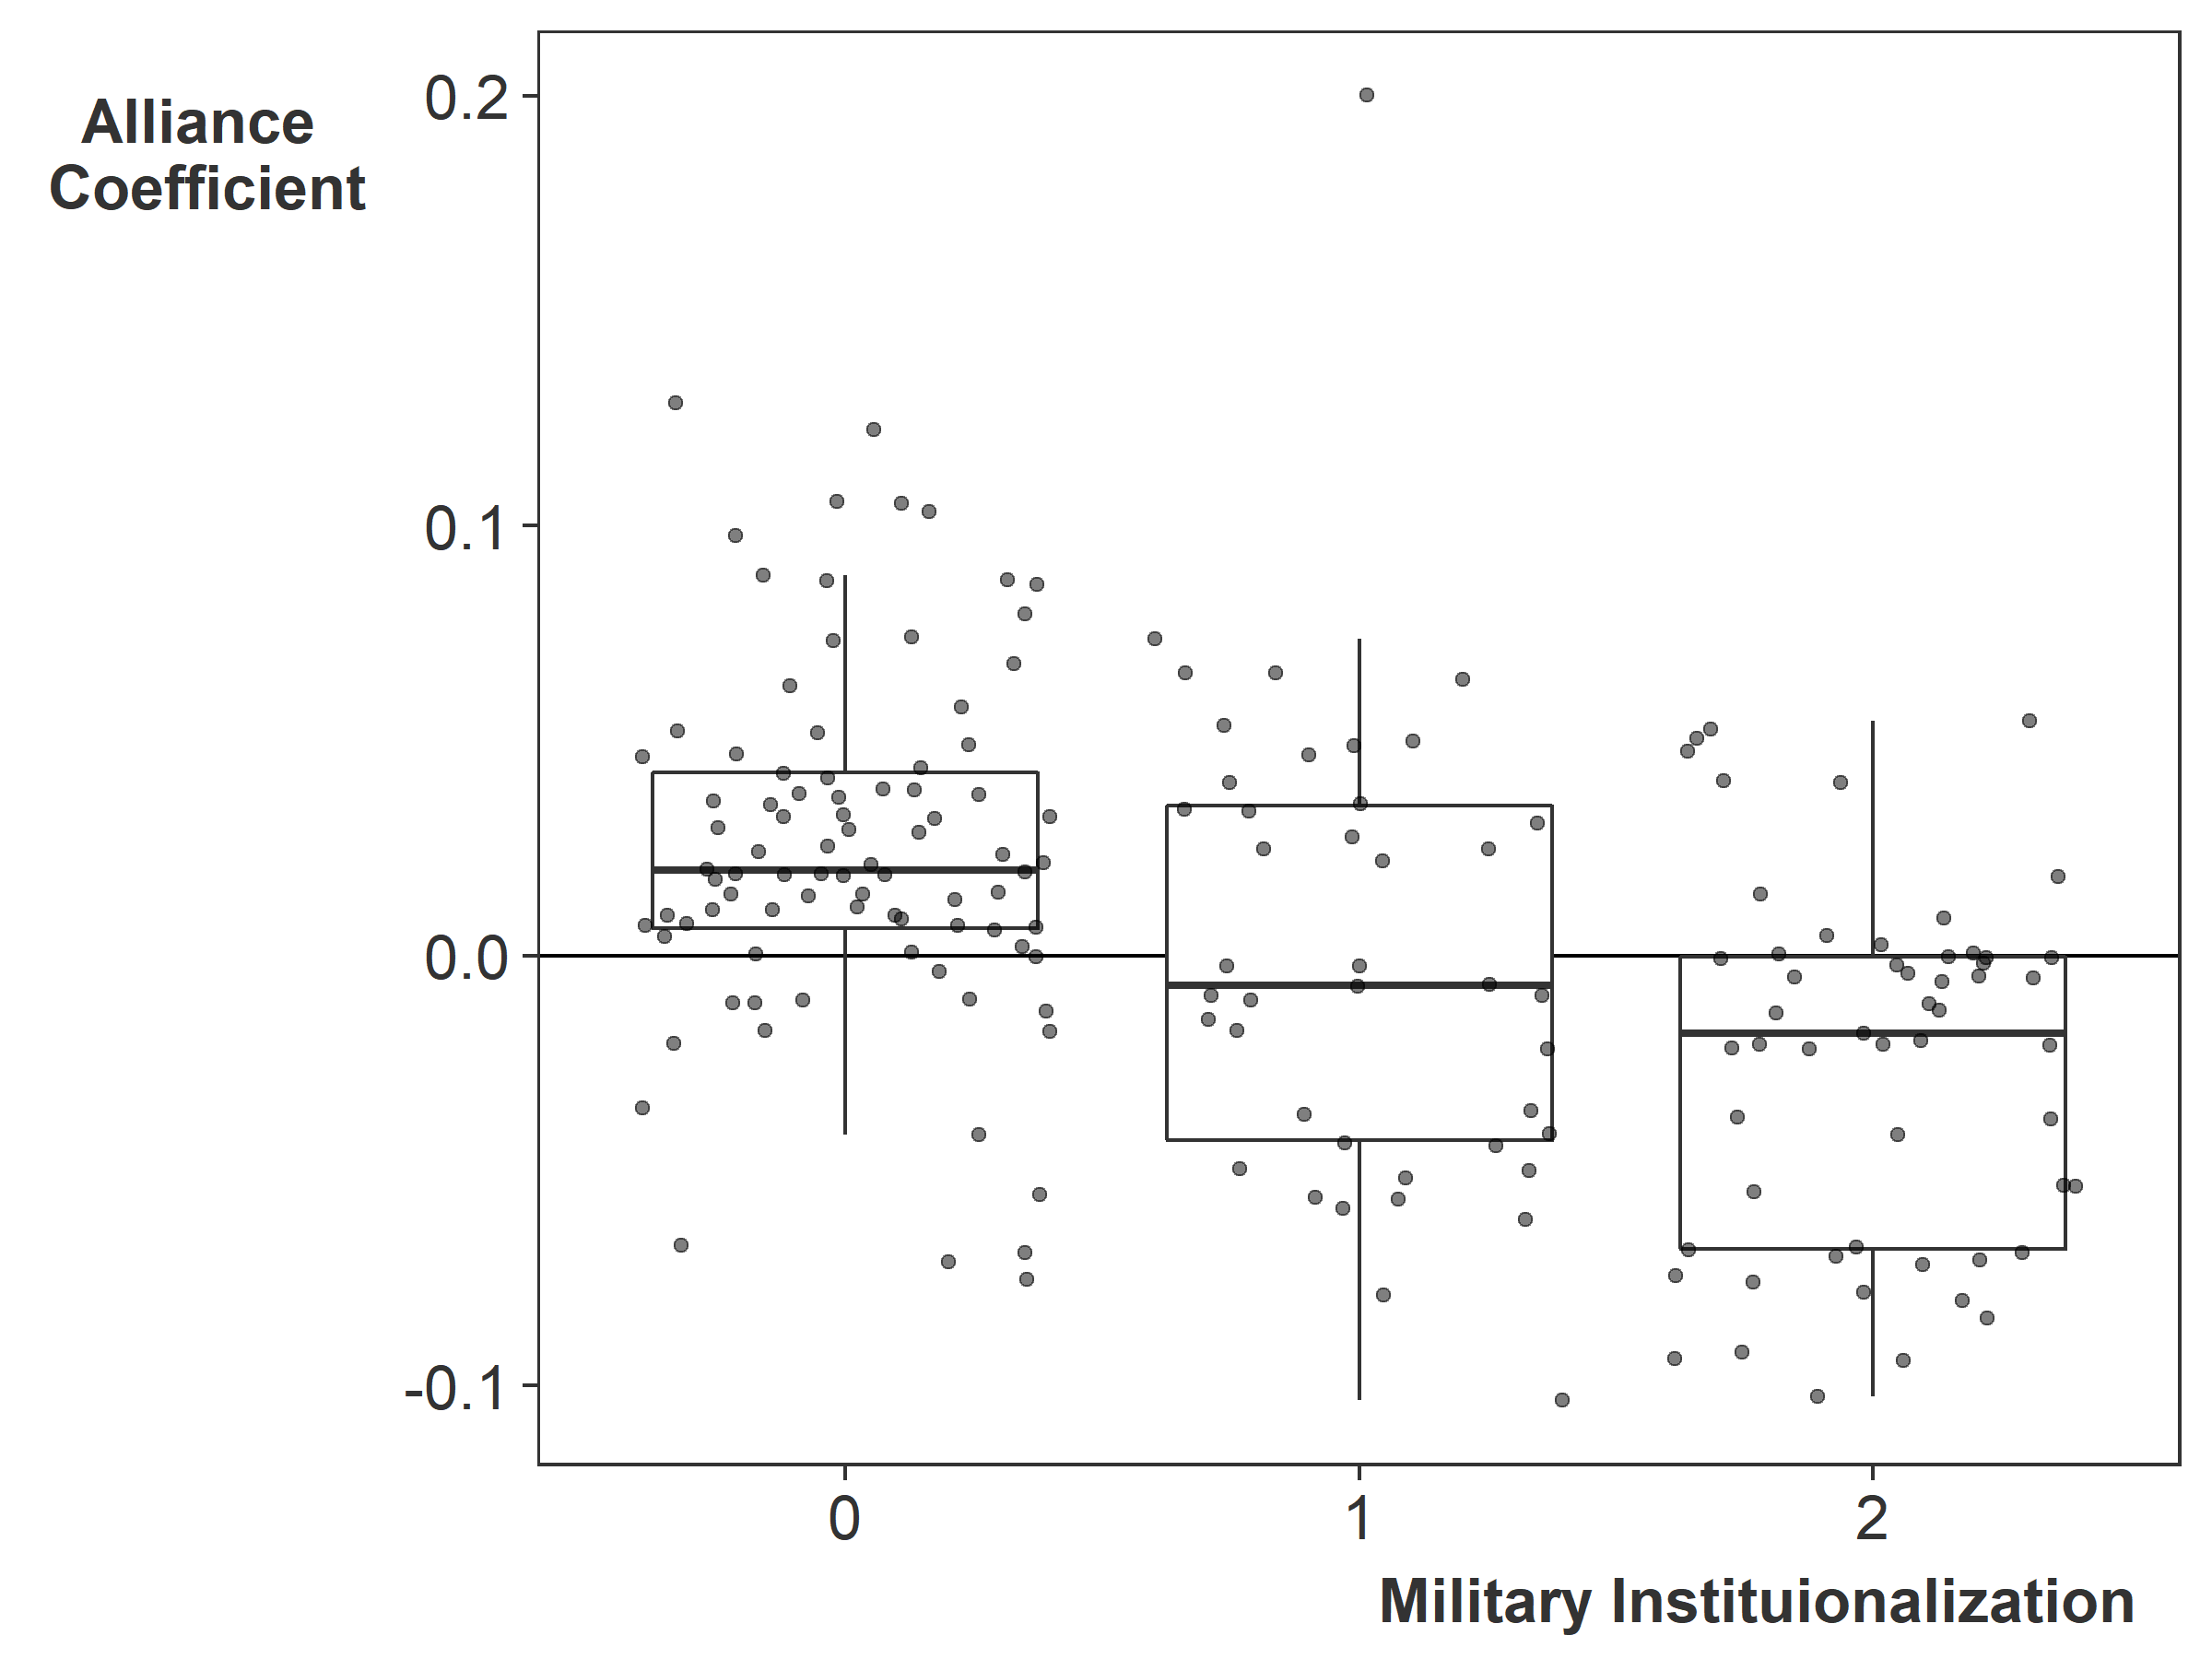
\includegraphics[width=0.95\textwidth]{milinst-lambda.png}
\end{figure}


\end{frame}

%-----------------------------------------------

\begin{frame}{Depth and First Year of the Alliance}

\begin{figure}
	\centering
		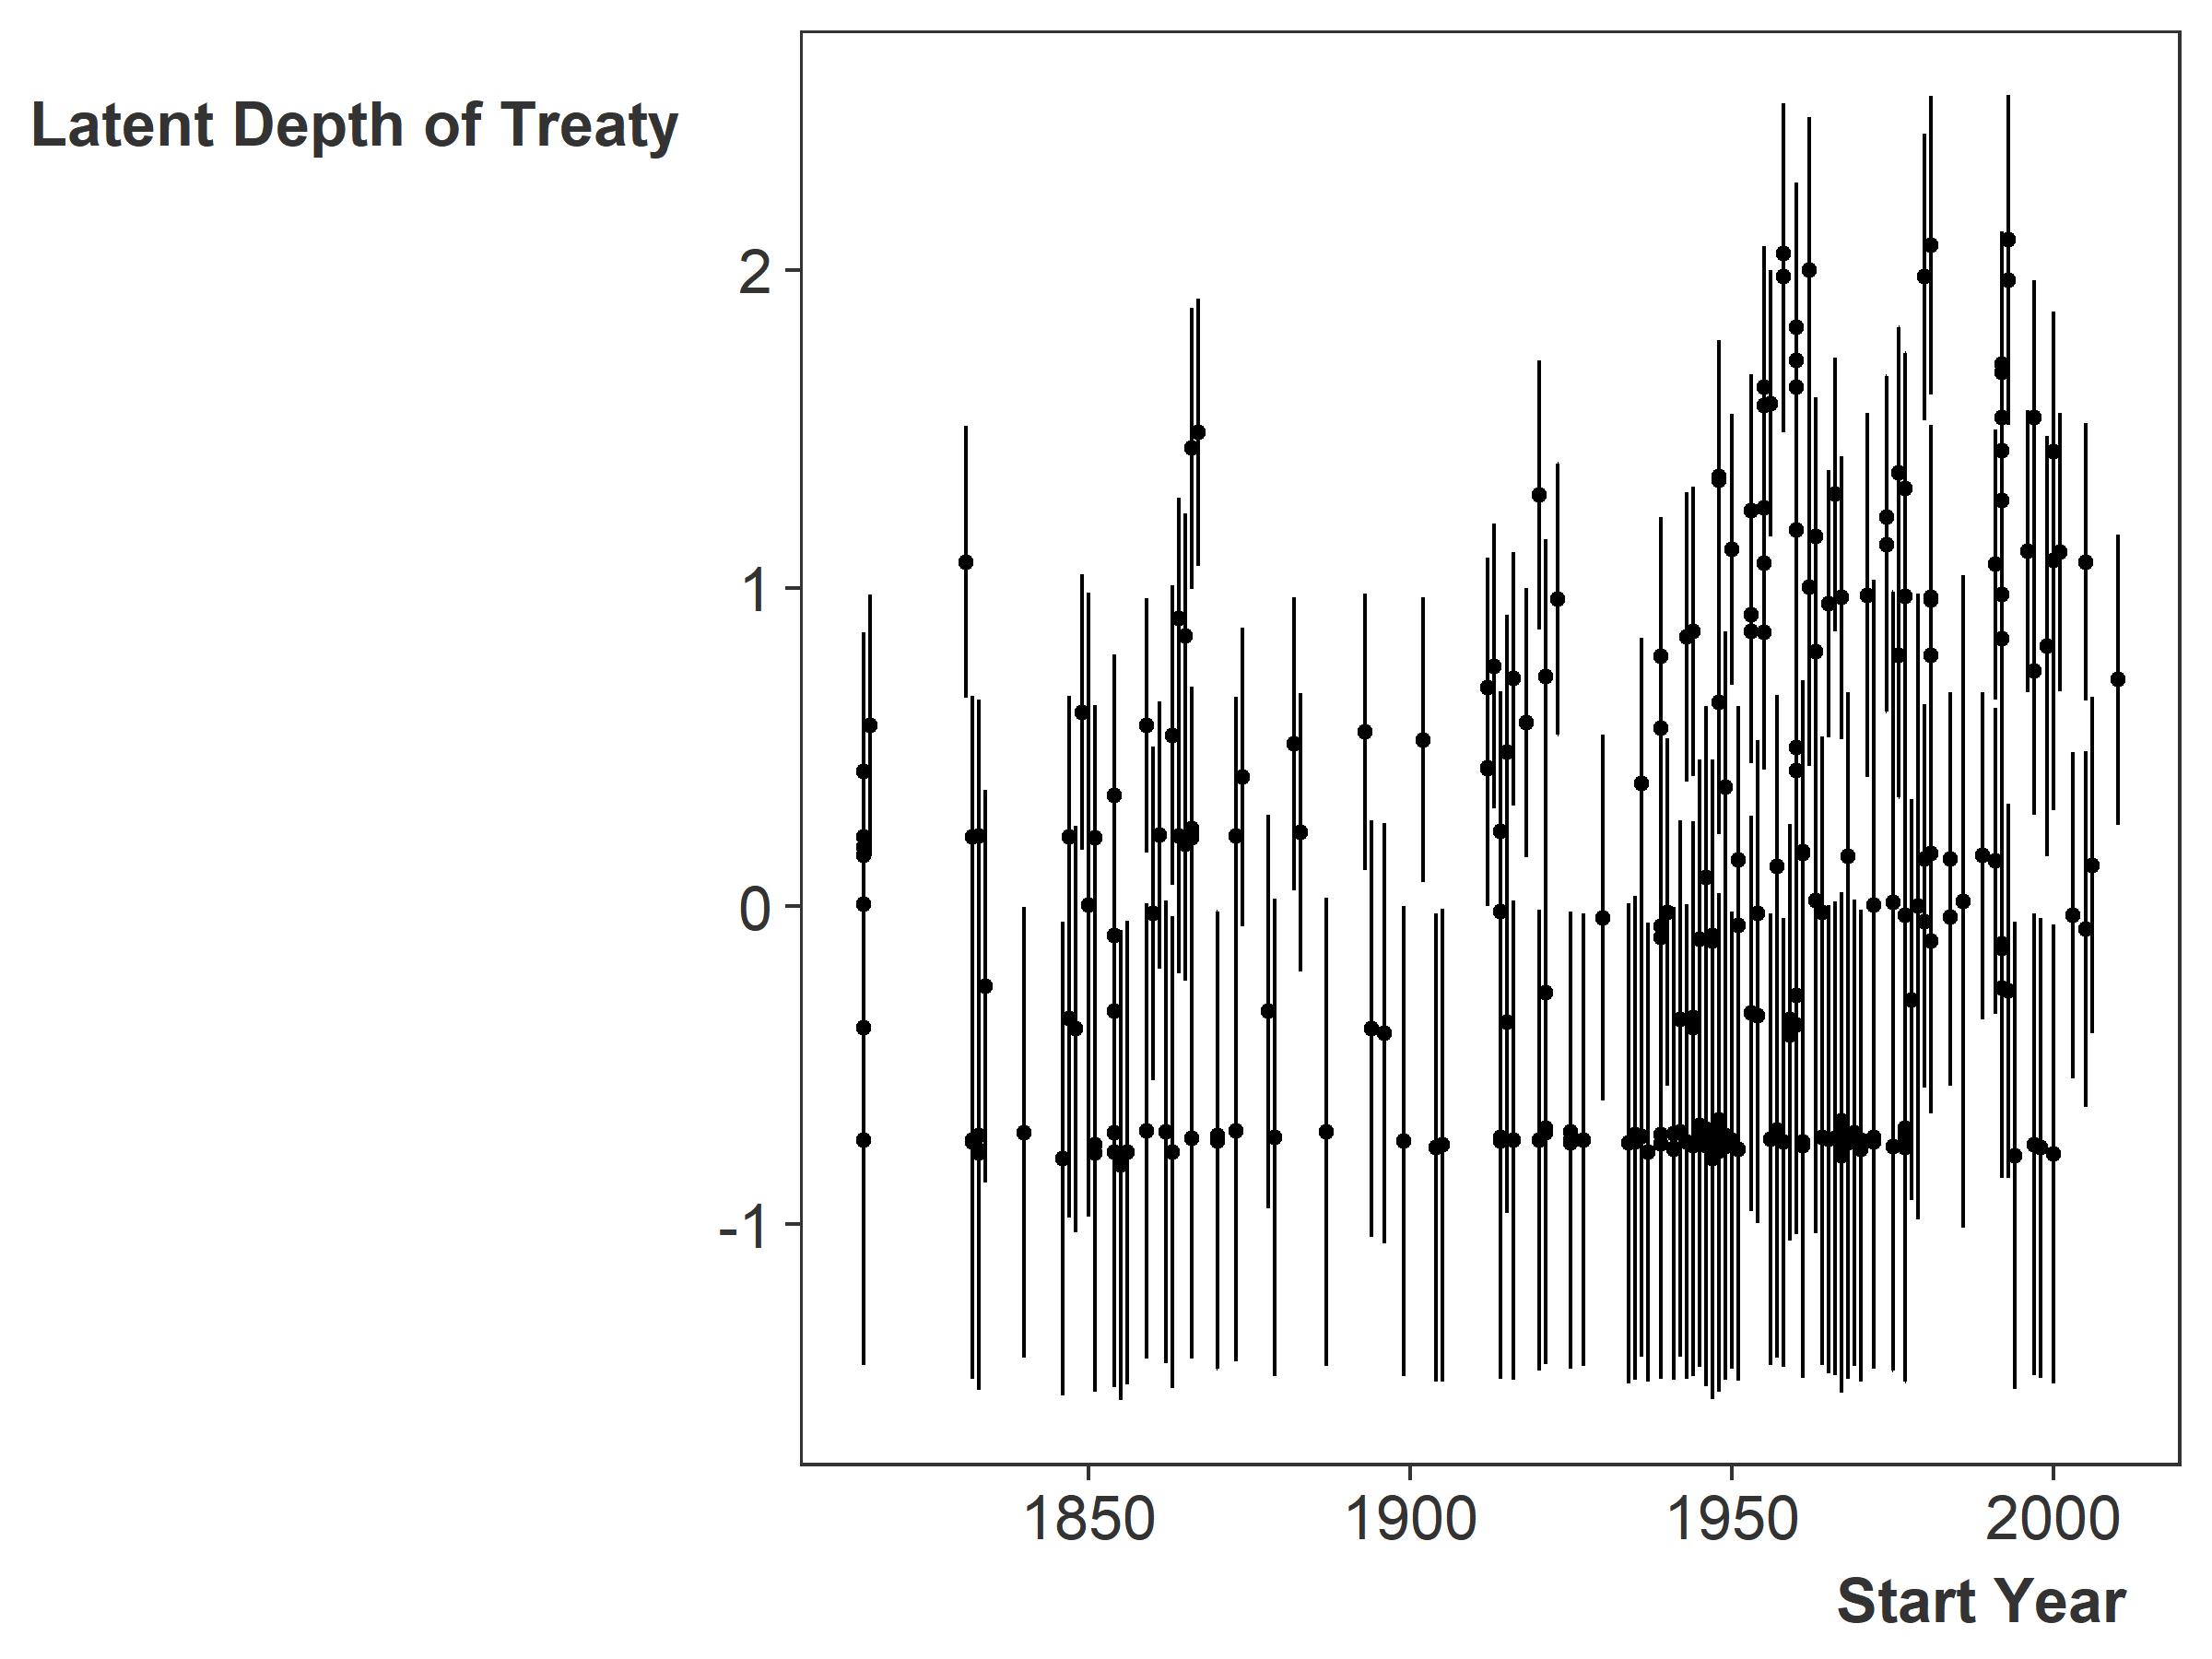
\includegraphics[width=0.95\textwidth]{ld-start-year.png}
\end{figure}


\end{frame}



%-----------------------------------------------

\begin{frame}{Trace plots: Non-Major}

\begin{figure}
	\centering
		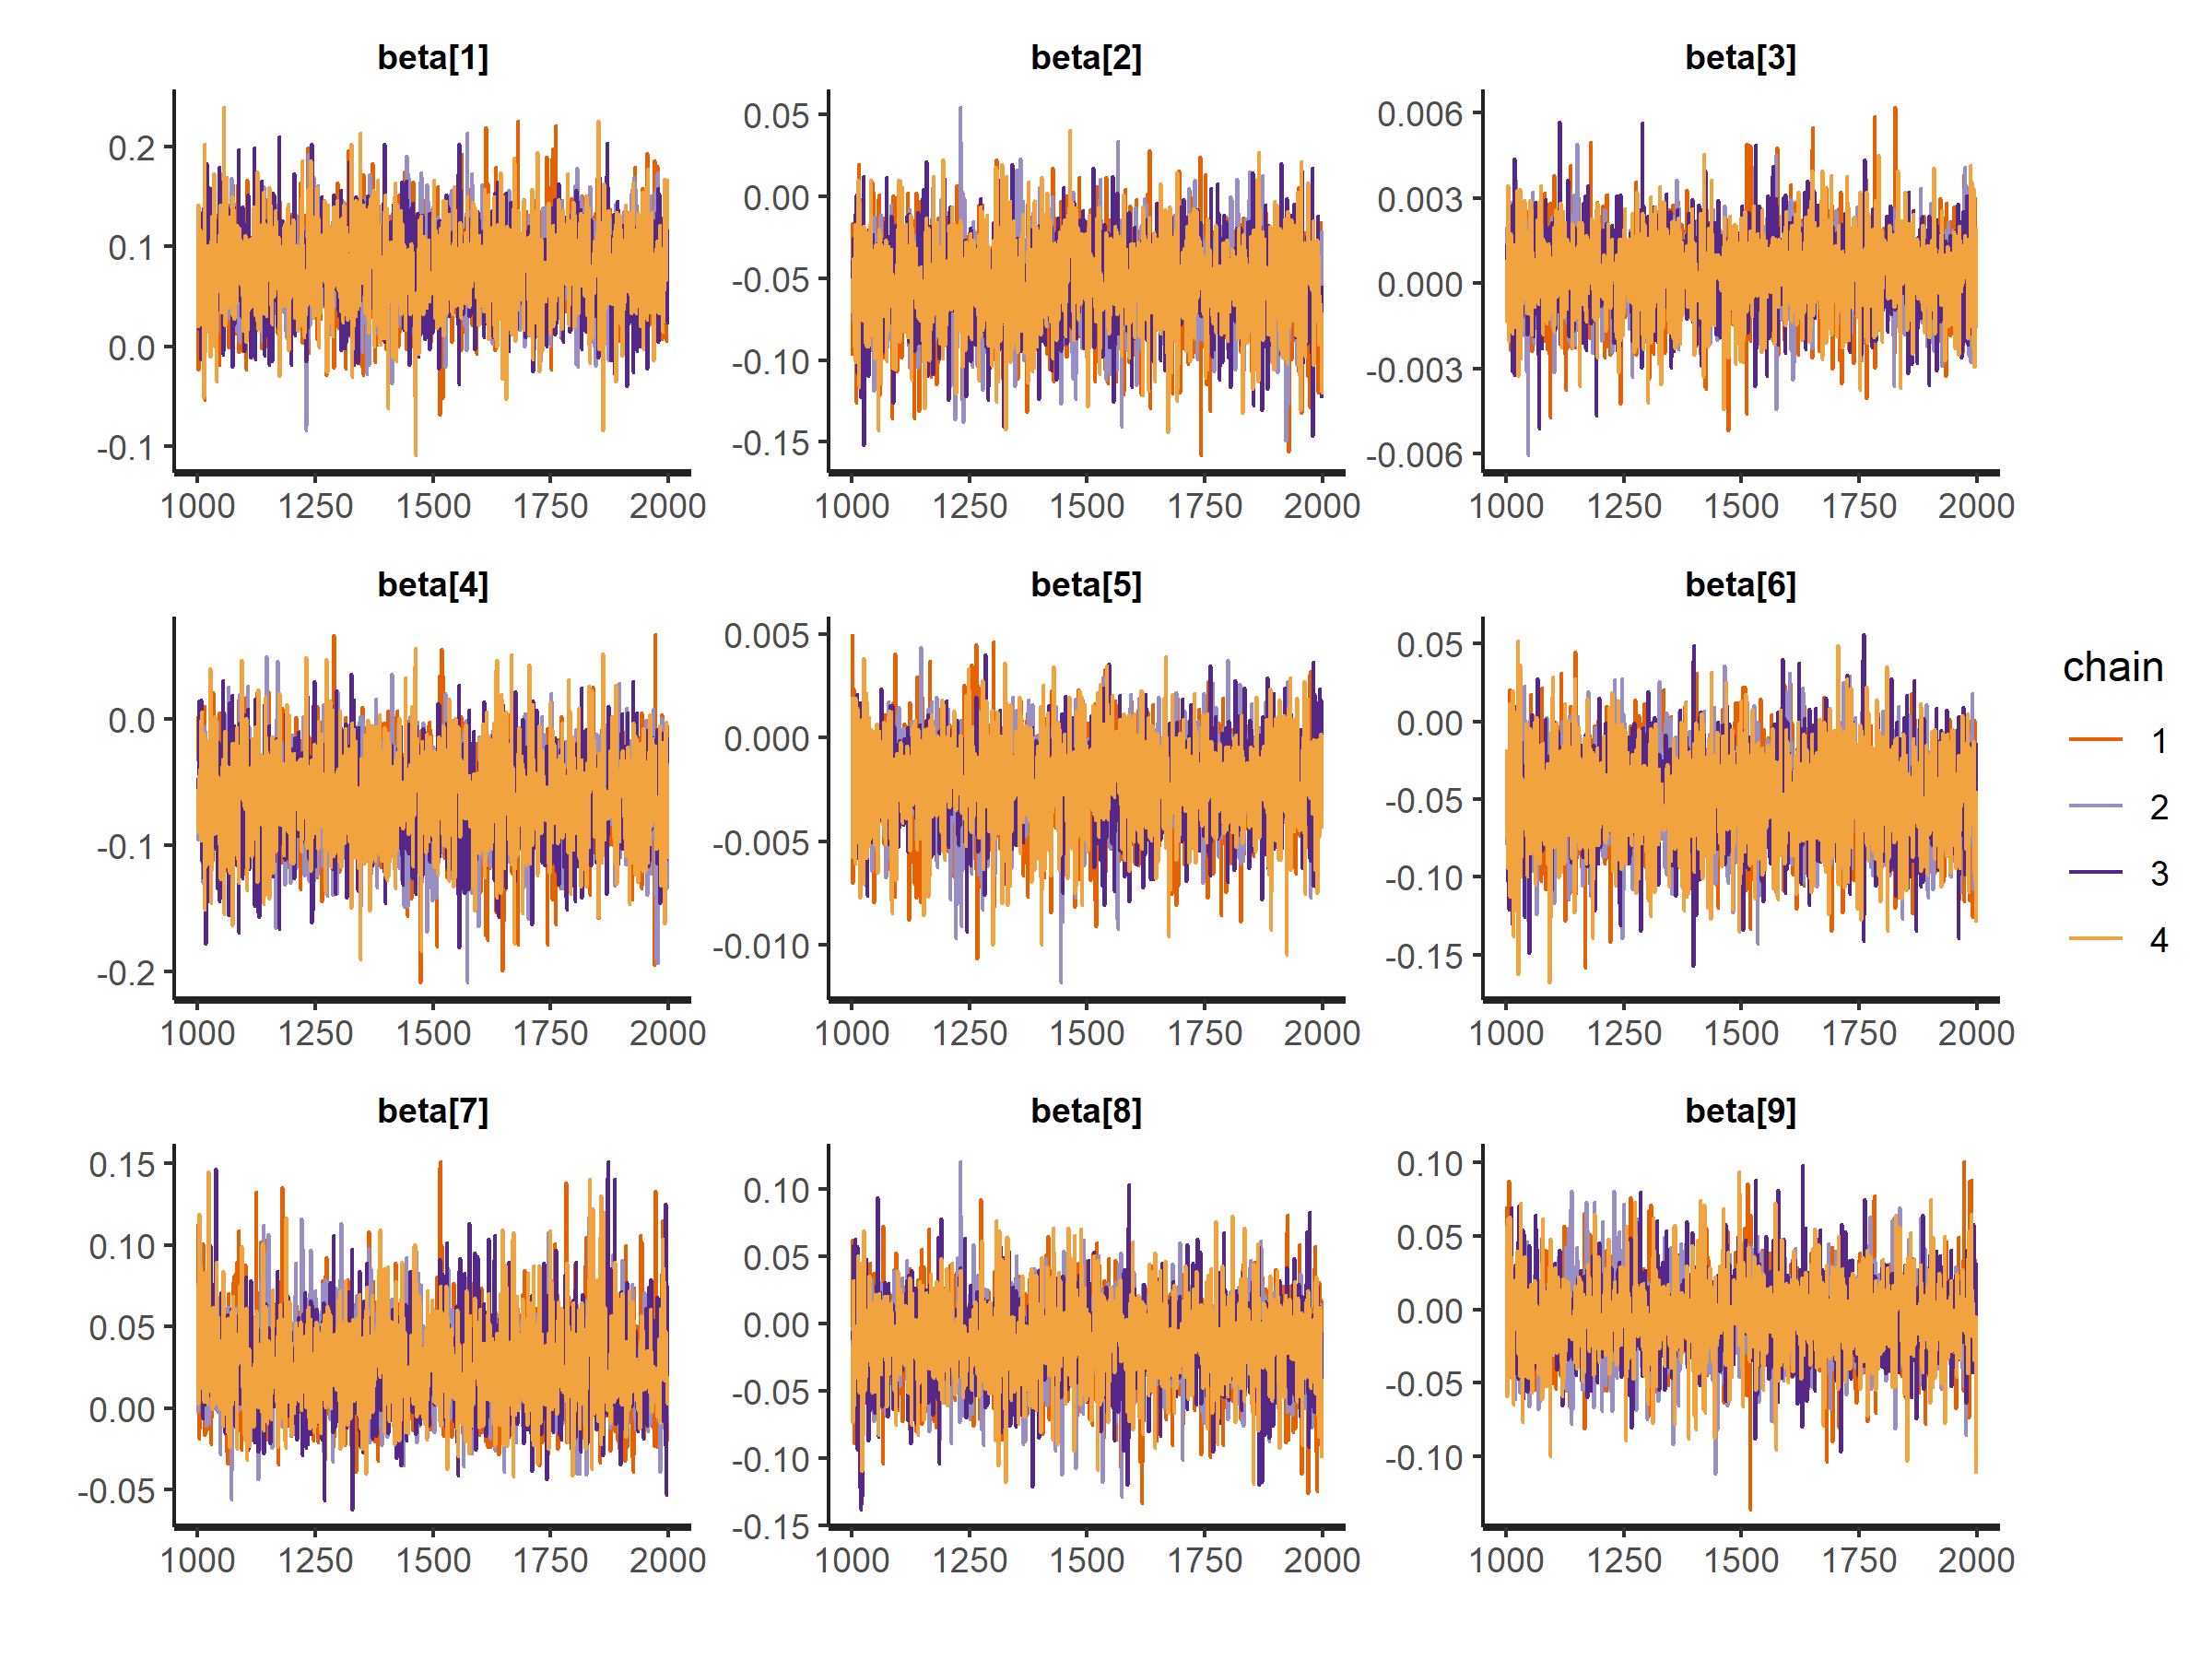
\includegraphics[width=0.95\textwidth]{beta-trace-maj.png}
\end{figure}


\end{frame}


%-----------------------------------------------

\begin{frame}{Model Check: Recovering Known Parameters}

Another way to check complicated models is simulating fake data with known parameters, then using the model to recover said parameters. 

To check my model, I simulated a dataset of 2,000 observations with 50 states, 200 years, 100 alliances and 4 variables: 2 at each level.

The 90\% credible intervals contain the known value for all regression parameters. 93 of 100 alliance specific parameter intervals contain the known value. 

\end{frame}


%-----------------------------------------------

\begin{frame}{Simulated Parameters and Credible Intervals}


\begin{figure}
	\centering
		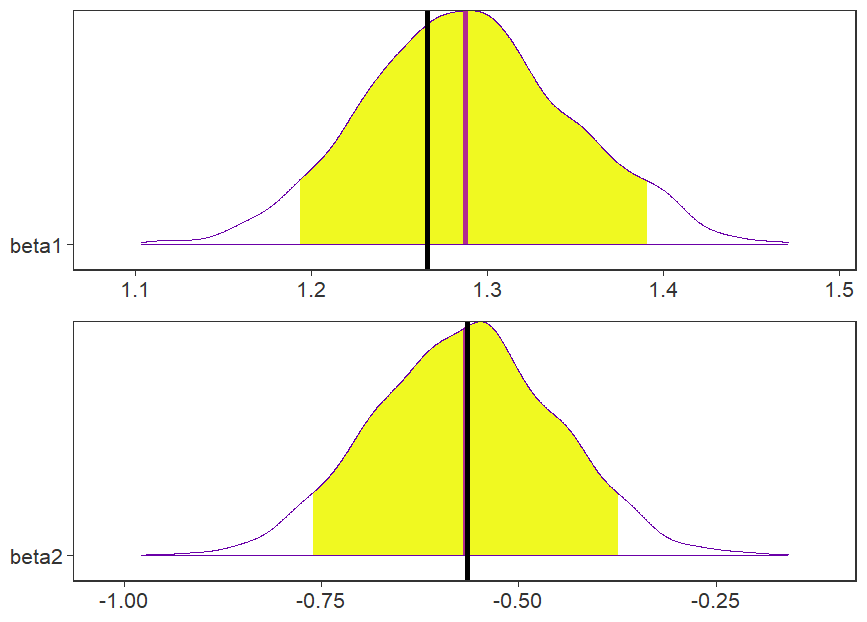
\includegraphics[width=0.95\textwidth]{sim-check-res.png}
\end{figure} 

\end{frame}



%-----------------------------------------------

\begin{frame}{Alliance-Level Regression Table: Non-Major Powers}

\resizebox{.95\textwidth}{!}{
\begin{tabular}{rrrrrrr}
  \hline
 & mean & sd & 5\% & 95\% & n\_eff & $\hat{R}$ \\ 
  \hline
Constant & -0.025 & 0.049 & -0.109 & 0.055 & 2332.133 & 1.000 \\ 
  Depth & -0.035 & 0.020 & -0.068 & -0.002 & 3566.248 & 1.000 \\ 
  Uncond Milsup & -0.020 & 0.038 & -0.084 & 0.041 & 3369.350 & 1.001 \\ 
  Econ. Link & 0.018 & 0.041 & -0.047 & 0.084 & 2597.771 & 1.002 \\ 
  FP Conc. & 0.030 & 0.021 & -0.005 & 0.063 & 3251.107 & 1.000 \\ 
  Number Members & 0.001 & 0.002 & -0.001 & 0.004 & 4309.891 & 1.001 \\ 
  FP Similarity & 0.017 & 0.058 & -0.078 & 0.111 & 2523.621 & 1.000 \\ 
  Democratic Membership & -0.001 & 0.004 & -0.007 & 0.005 & 2843.301 & 1.002 \\ 
  Wartime & 0.047 & 0.048 & -0.030 & 0.125 & 3921.848 & 1.002 \\ 
  Asymmetric & 0.039 & 0.055 & -0.048 & 0.130 & 3165.178 & 1.001 \\ 
  US. Mem & -0.044 & 0.043 & -0.110 & 0.027 & 2603.217 & 1.000 \\ 
  USSR Mem. & -0.129 & 0.091 & -0.276 & 0.021 & 2826.512 & 1.001 \\ 
  $\sigma$ Alliances & 0.118 & 0.050 & 0.037 & 0.203 & 746.918 & 1.004 \\ 
   \hline
\end{tabular}
}


\end{frame}


%------------------------------------------------

\begin{frame}{Treaty Depth and Other Alliance Characteristics}

\begin{figure}
	\centering
		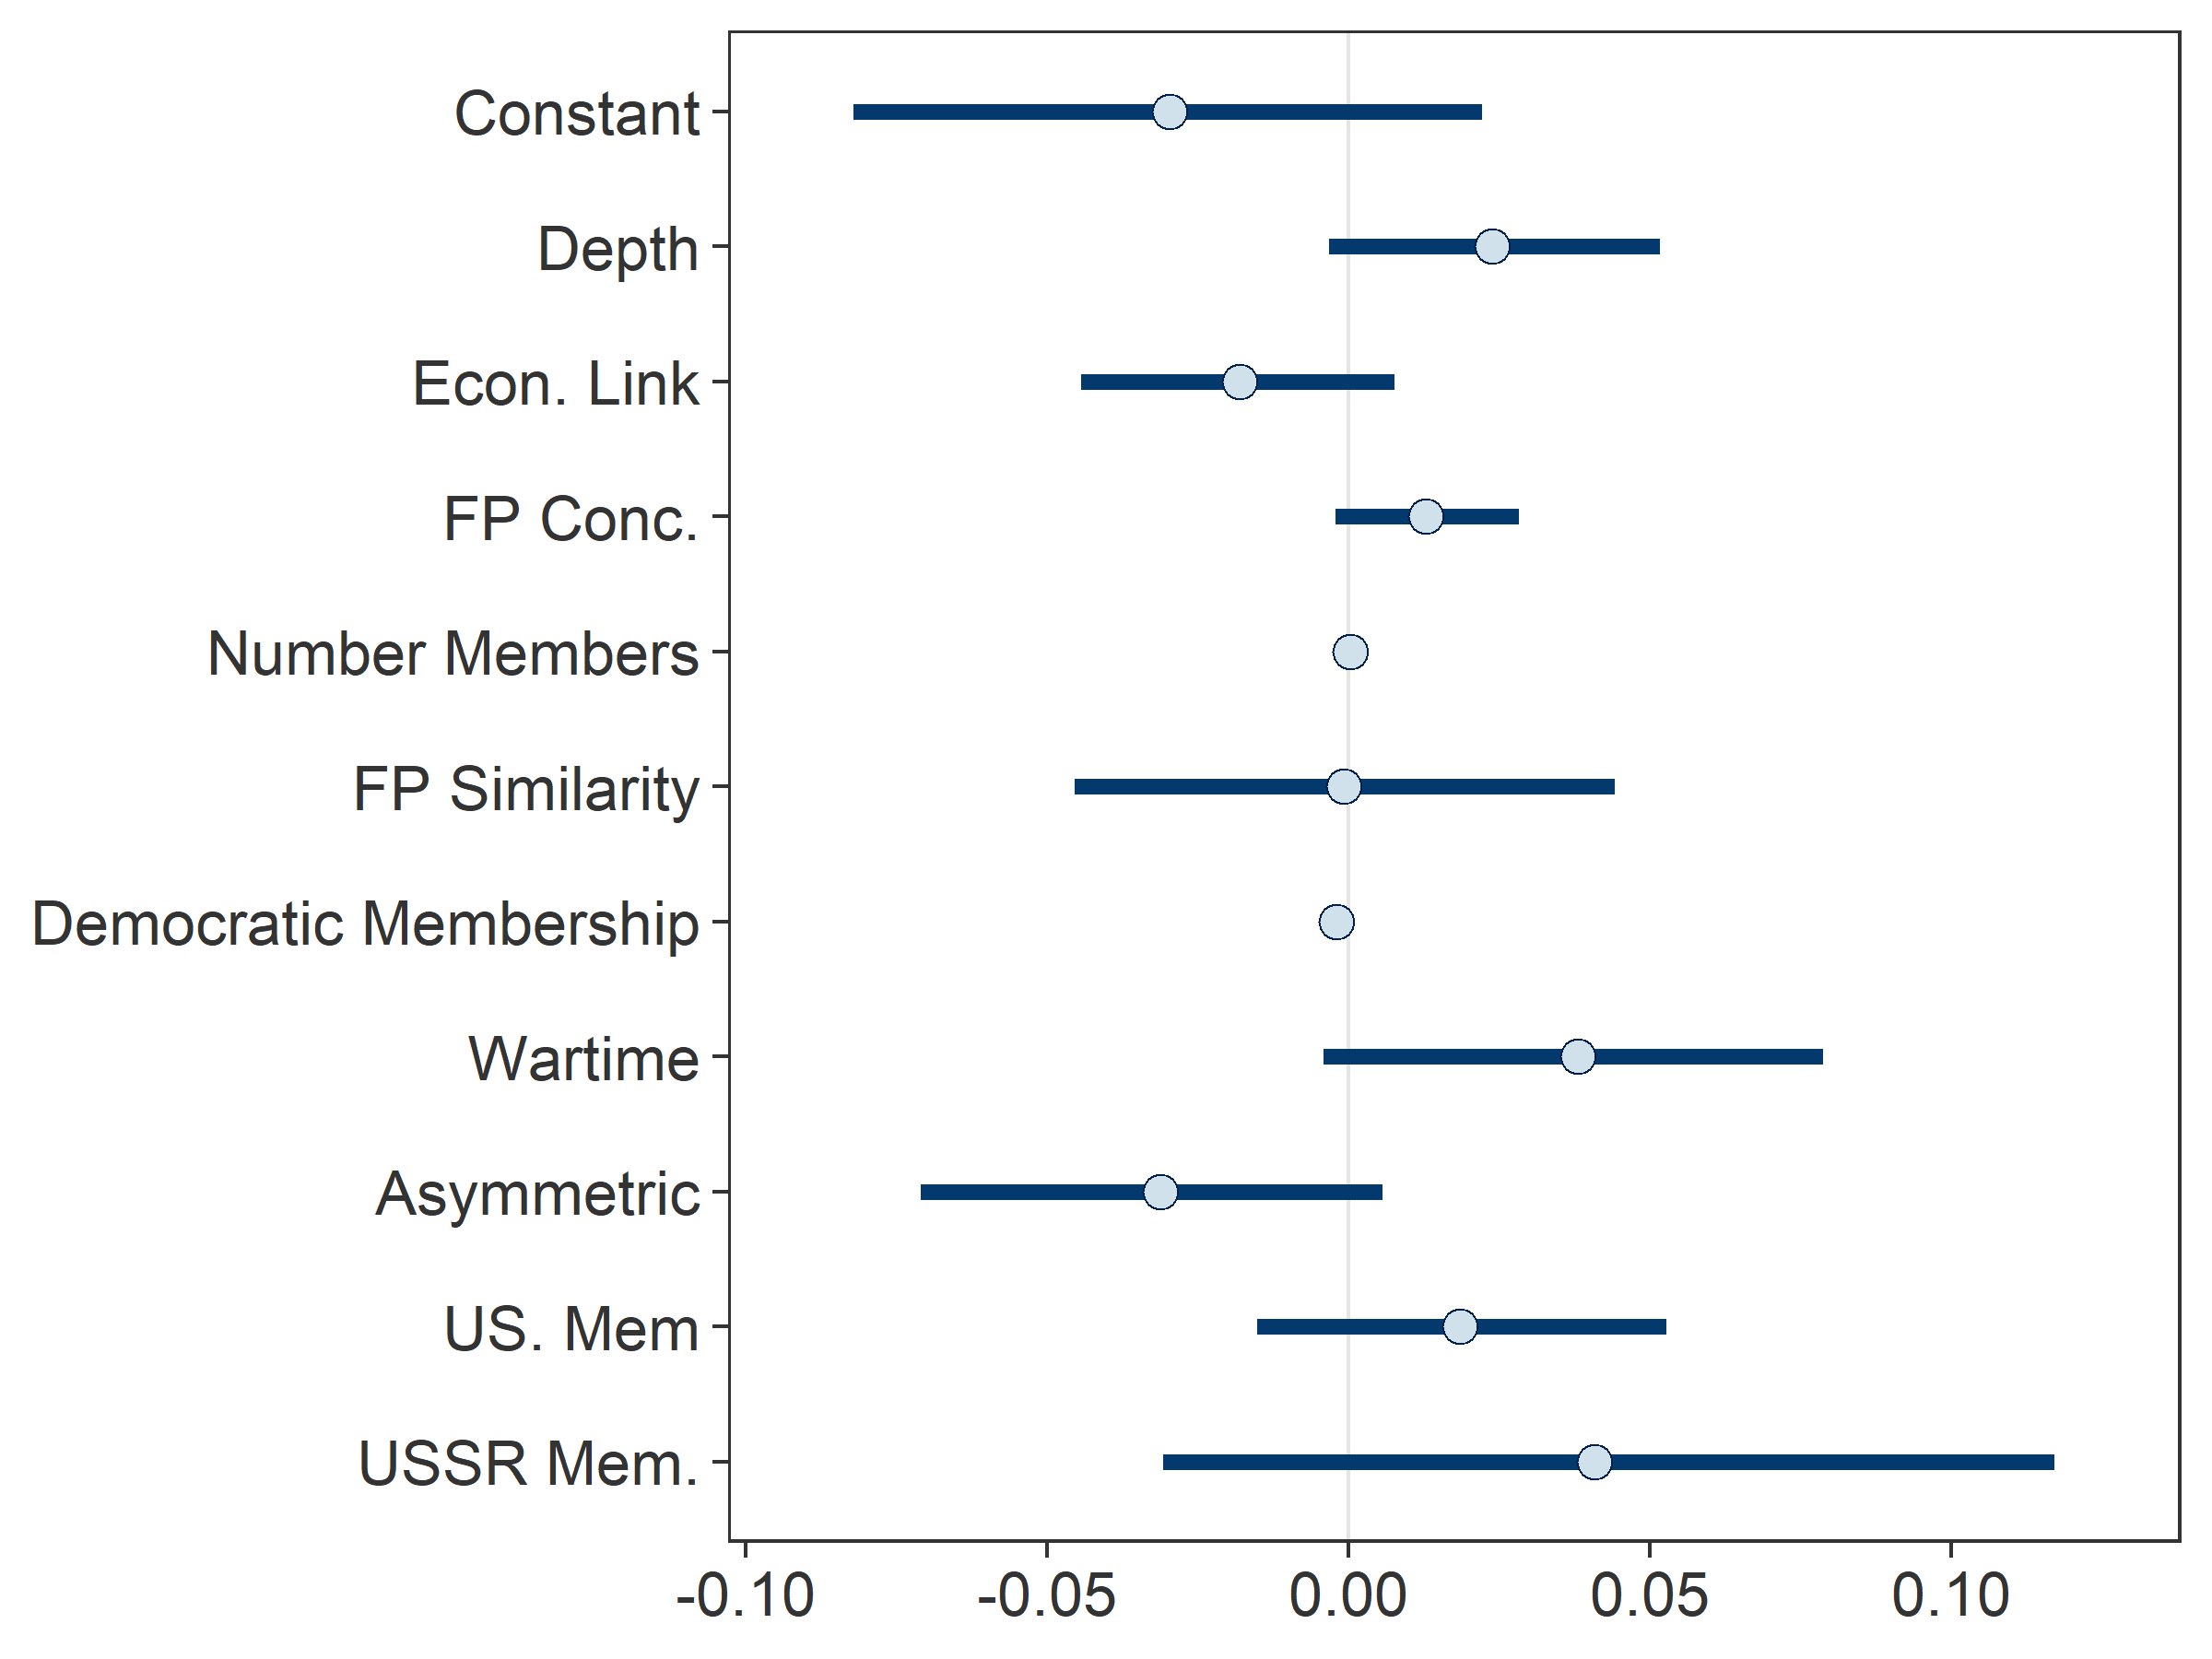
\includegraphics[width=0.9\textwidth]{beta-intervals-min.png}
	\label{fig:beta-intervals-min}
\end{figure}


\end{frame}

%------------------------------------------------


\begin{frame}{Priors}

4 Chains with 2,000 samples and 1,000 warmup iterations. 

\begin{table} % Create a table of priors.

 \begin{center}
\begin{tabular}{c} 
$ p(\alpha) \sim N(0, 1)$  \\
$ p(\sigma) \sim \mbox{half-}N(0, 1) $ \\
$ p(\alpha^{yr}) \sim N(0, \sigma^{yr}) $ \\ 
$ p(\sigma^{yr}) \sim N(0, 1) $ \\
$ p(\alpha^{st}) \sim N(0, \sigma^{st}) $ \\ 
$ p(\sigma^{st}) \sim \mbox{half-}N(0, .5) $ \\ 
$ p(\sigma^{all}) \sim \mbox{half-}N(0, .5) $ \\
$ p(\beta) \sim N(0, .5) $ \\
$ p(\gamma) \sim N(0, .5) $ \\ 
$ p(\nu) \sim gamma(2, 0.1)$ 
\end{tabular} 
\end{center} 
\label{tab:priors}
\end{table} 


\end{frame}


%------------------------------------------------


\begin{frame}{ML Model Specification}

\begin{equation}
y \sim student_t(\nu, \mu, \sigma)
\end{equation}
\begin{equation}
\mu = \alpha + \alpha^{st} + \alpha^{yr} +\textbf{W}_{n \times k} \gamma + \textbf{Z}_{n \times a} \lambda
\end{equation}

\begin{equation}
\lambda_{a} \sim N(\theta_{a}, \sigma_{all})
\end{equation}
\begin{equation}
\theta_a = \alpha_{all} + \beta_1 \mbox{Treaty Depth} + \textbf{X}_{a \times l} \beta
\end{equation}


\end{frame}


%------------------------------------------------

\begin{frame}{Example}

\setbeamercovered{transparent}

\begin{equation*}
\uncover<2->{\mu_{it} =} \uncover<3>{\alpha} \uncover<4>{+ \alpha^{st} + \alpha^{yr}} \uncover<5>{+ W_{it} \gamma} \uncover<6>{+ Z_{it} \lambda}
\end{equation*}

Example year: Argentina 1955

\begin{equation*}
\begin{split}
& \uncover<2->{\mbox{1955 \% Change Milex.} = } \uncover<3>{\mbox{Overall mean}} \\
& \uncover<4>{+ \mbox{Argentine Intercept} + \mbox{1955 Intercept}} \\
& \uncover<5>{+ \mbox{Argentine Characteristics}} \\
& \uncover<6>{+ \lambda_{OAS} * \mbox{OAS Expenditure} + \lambda_{Rio} * \mbox{Rio Pact Expenditure}}
\end{split}
\end{equation*}

\uncover<7>{
\begin{equation*}
\lambda_{OAS} = \alpha_{all} + \beta_1 -0.11 + \mbox{Controls}
\end{equation*}
} 


\end{frame}




%------------------------------------------------


\begin{frame}[standout]{Z} 

\begin{tabular}{lccc}
State-Year & Rio Pact & Warsaw Pact & \ldots \\
\hline
Argentina 1954 & .347 & 0 & \ldots \\
Argentina 1955 & .418  & 0 & \ldots  \\
 \vdots & \vdots & \vdots & \ldots  
\end{tabular}

 \end{frame}
 
 
 %------------------------------------------------


\begin{frame}{Choice of Capability in Z} 

Used leave-one-out cross validation to assess model fit with different codings of \textbf{Z}. 

\begin{center}
\begin{tabular}{rrrrrrrrr}
  \hline
 Allied Capability & elpd\_diff & se\_diff & elpd\_loo & se\_elpd\_loo  \\ 
  \hline
  Normalized by Year & 0.000 & 0.000 & -1159.513 & 184.714 \\ 
  Rescaled by Maximum & -3.165 & 2.643 & -1162.679 & 184.723  \\ 
  Recaled by 2SD & -10.749 & 6.116 & -1170.262 & 184.741  \\ 
  Total Allied CINC & -12.308 & 5.576 & -1171.821 & 184.683  \\ 
   \hline
\end{tabular}
\end{center} 

 \end{frame}




%------------------------------------------------

\begin{frame}{Notable Major Power Alliances}


\begin{figure}
	\centering
		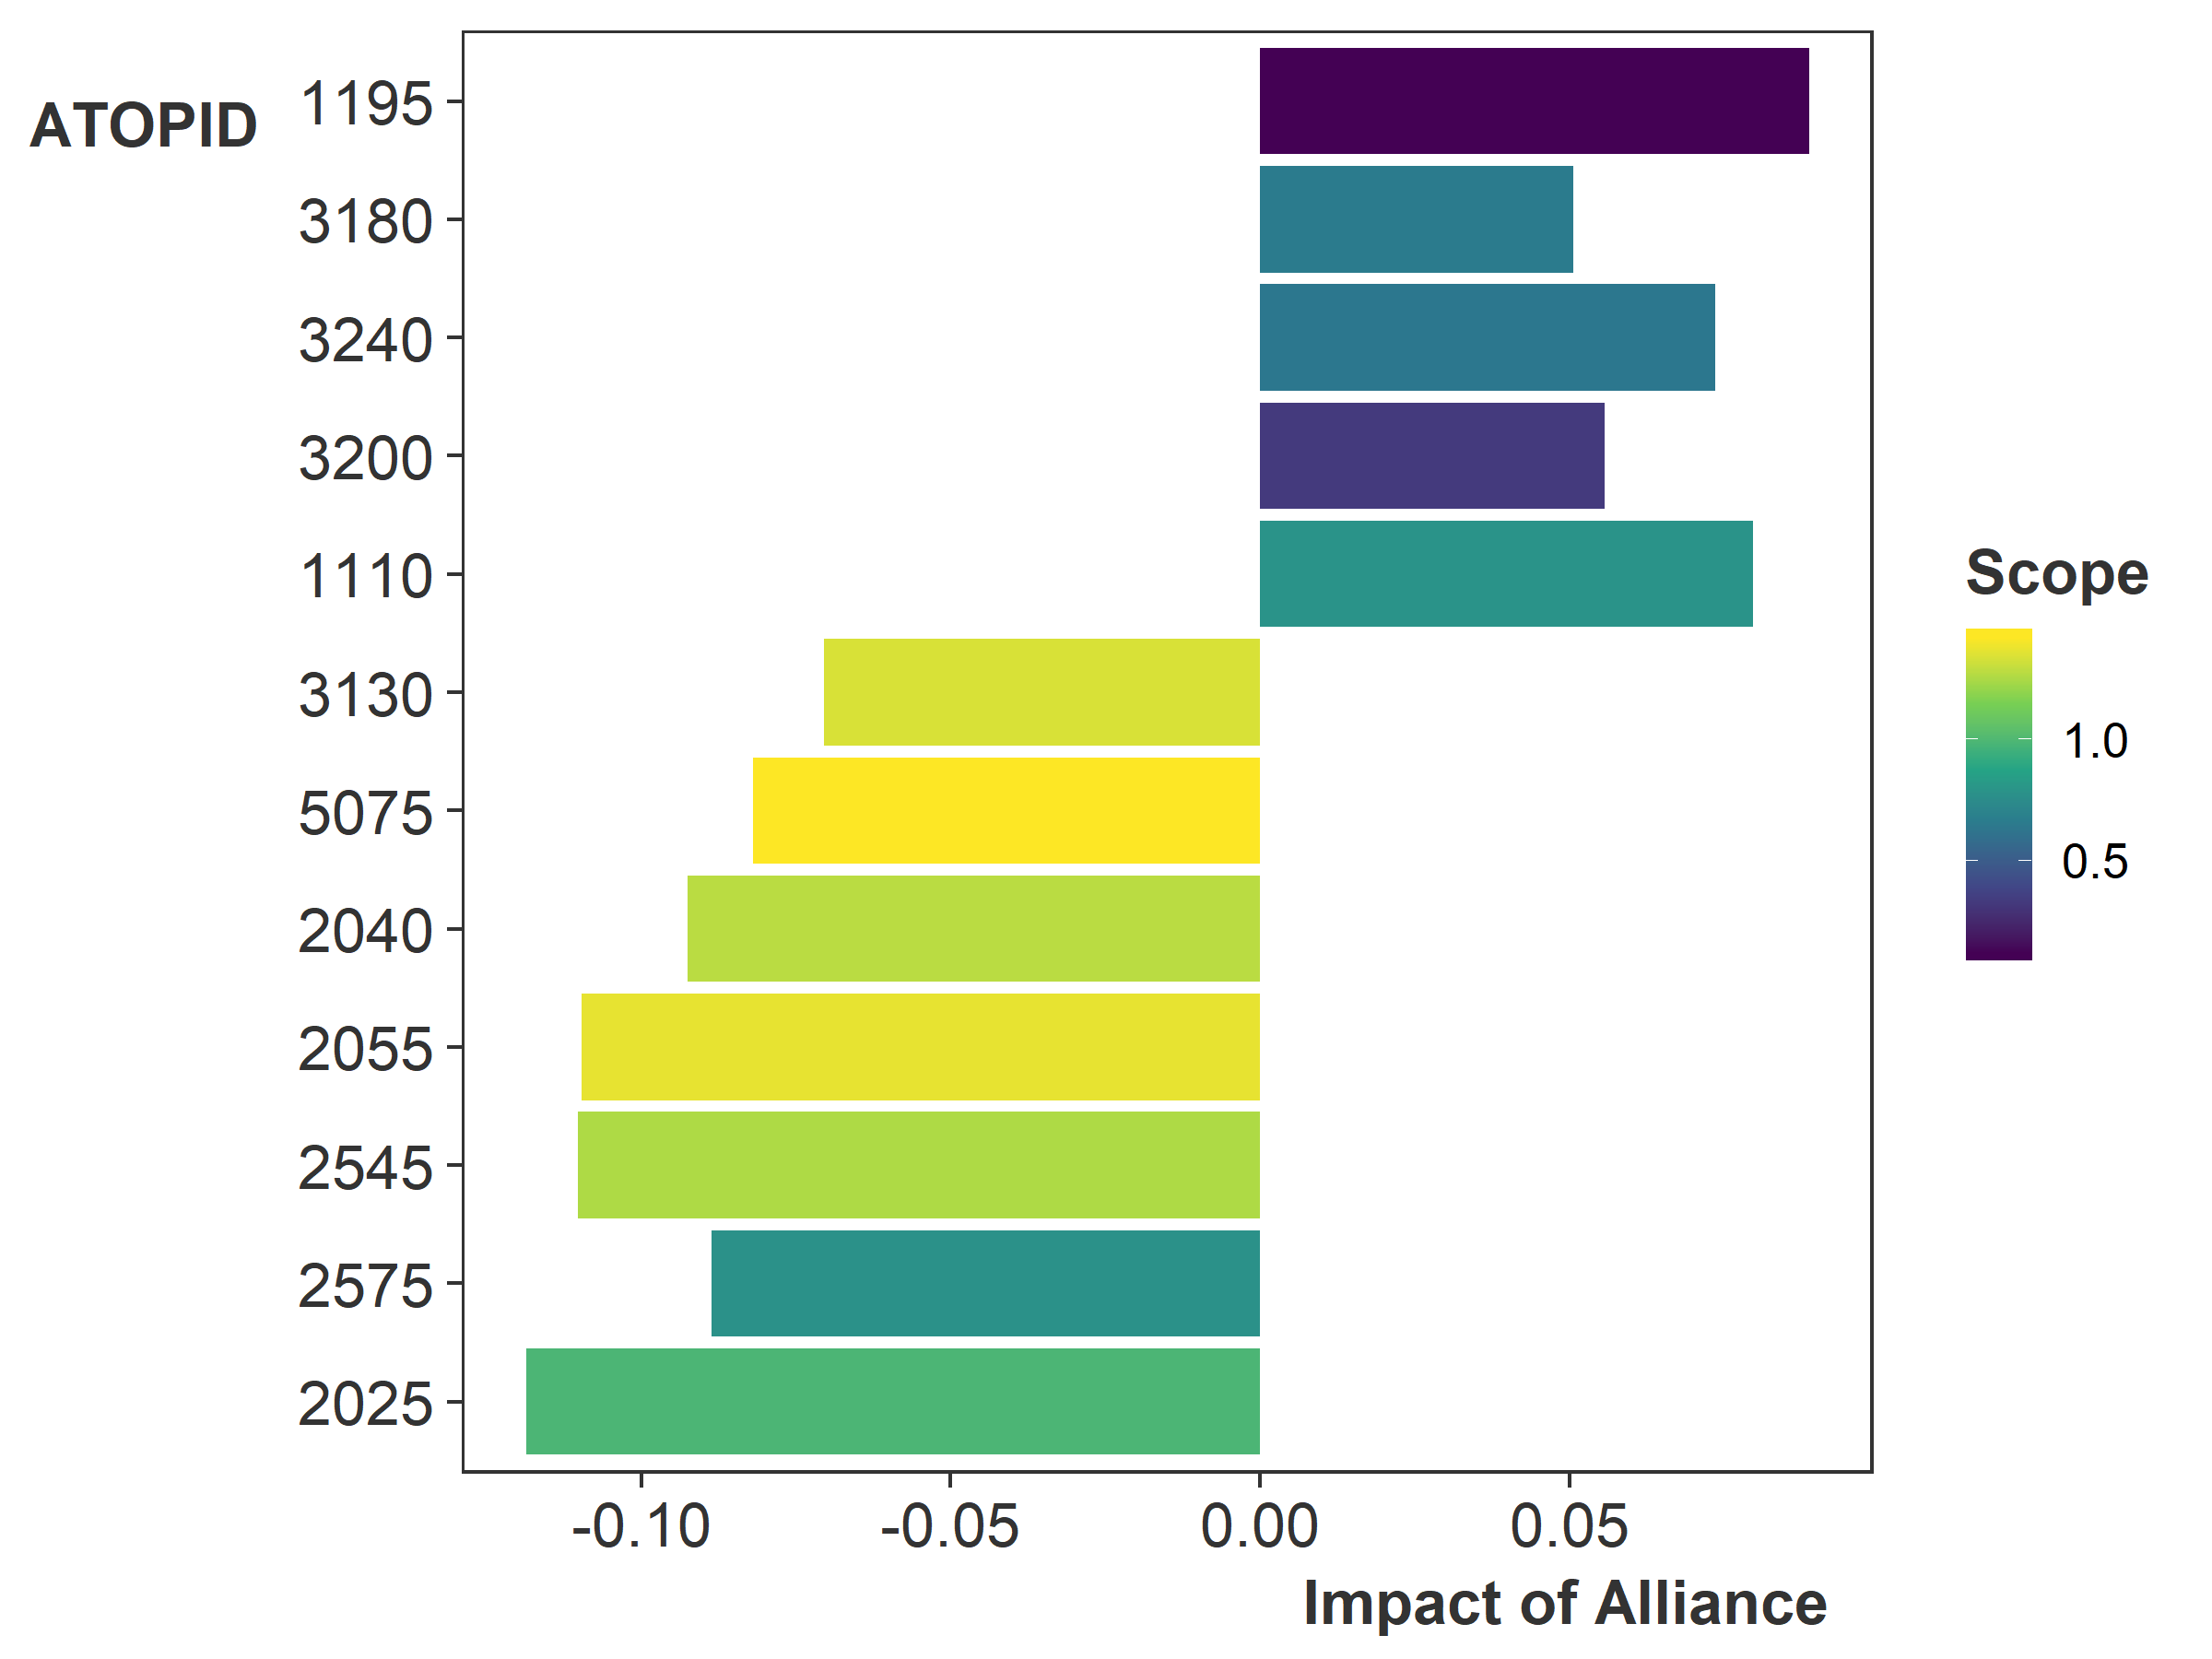
\includegraphics[width=0.95\textwidth]{non-zero-maj.png}
	\label{fig:non-zero-maj}
\end{figure}


\end{frame}

%------------------------------------------------

\begin{frame}{Notable Non-Major Power Alliances}


\begin{figure}
	\centering
		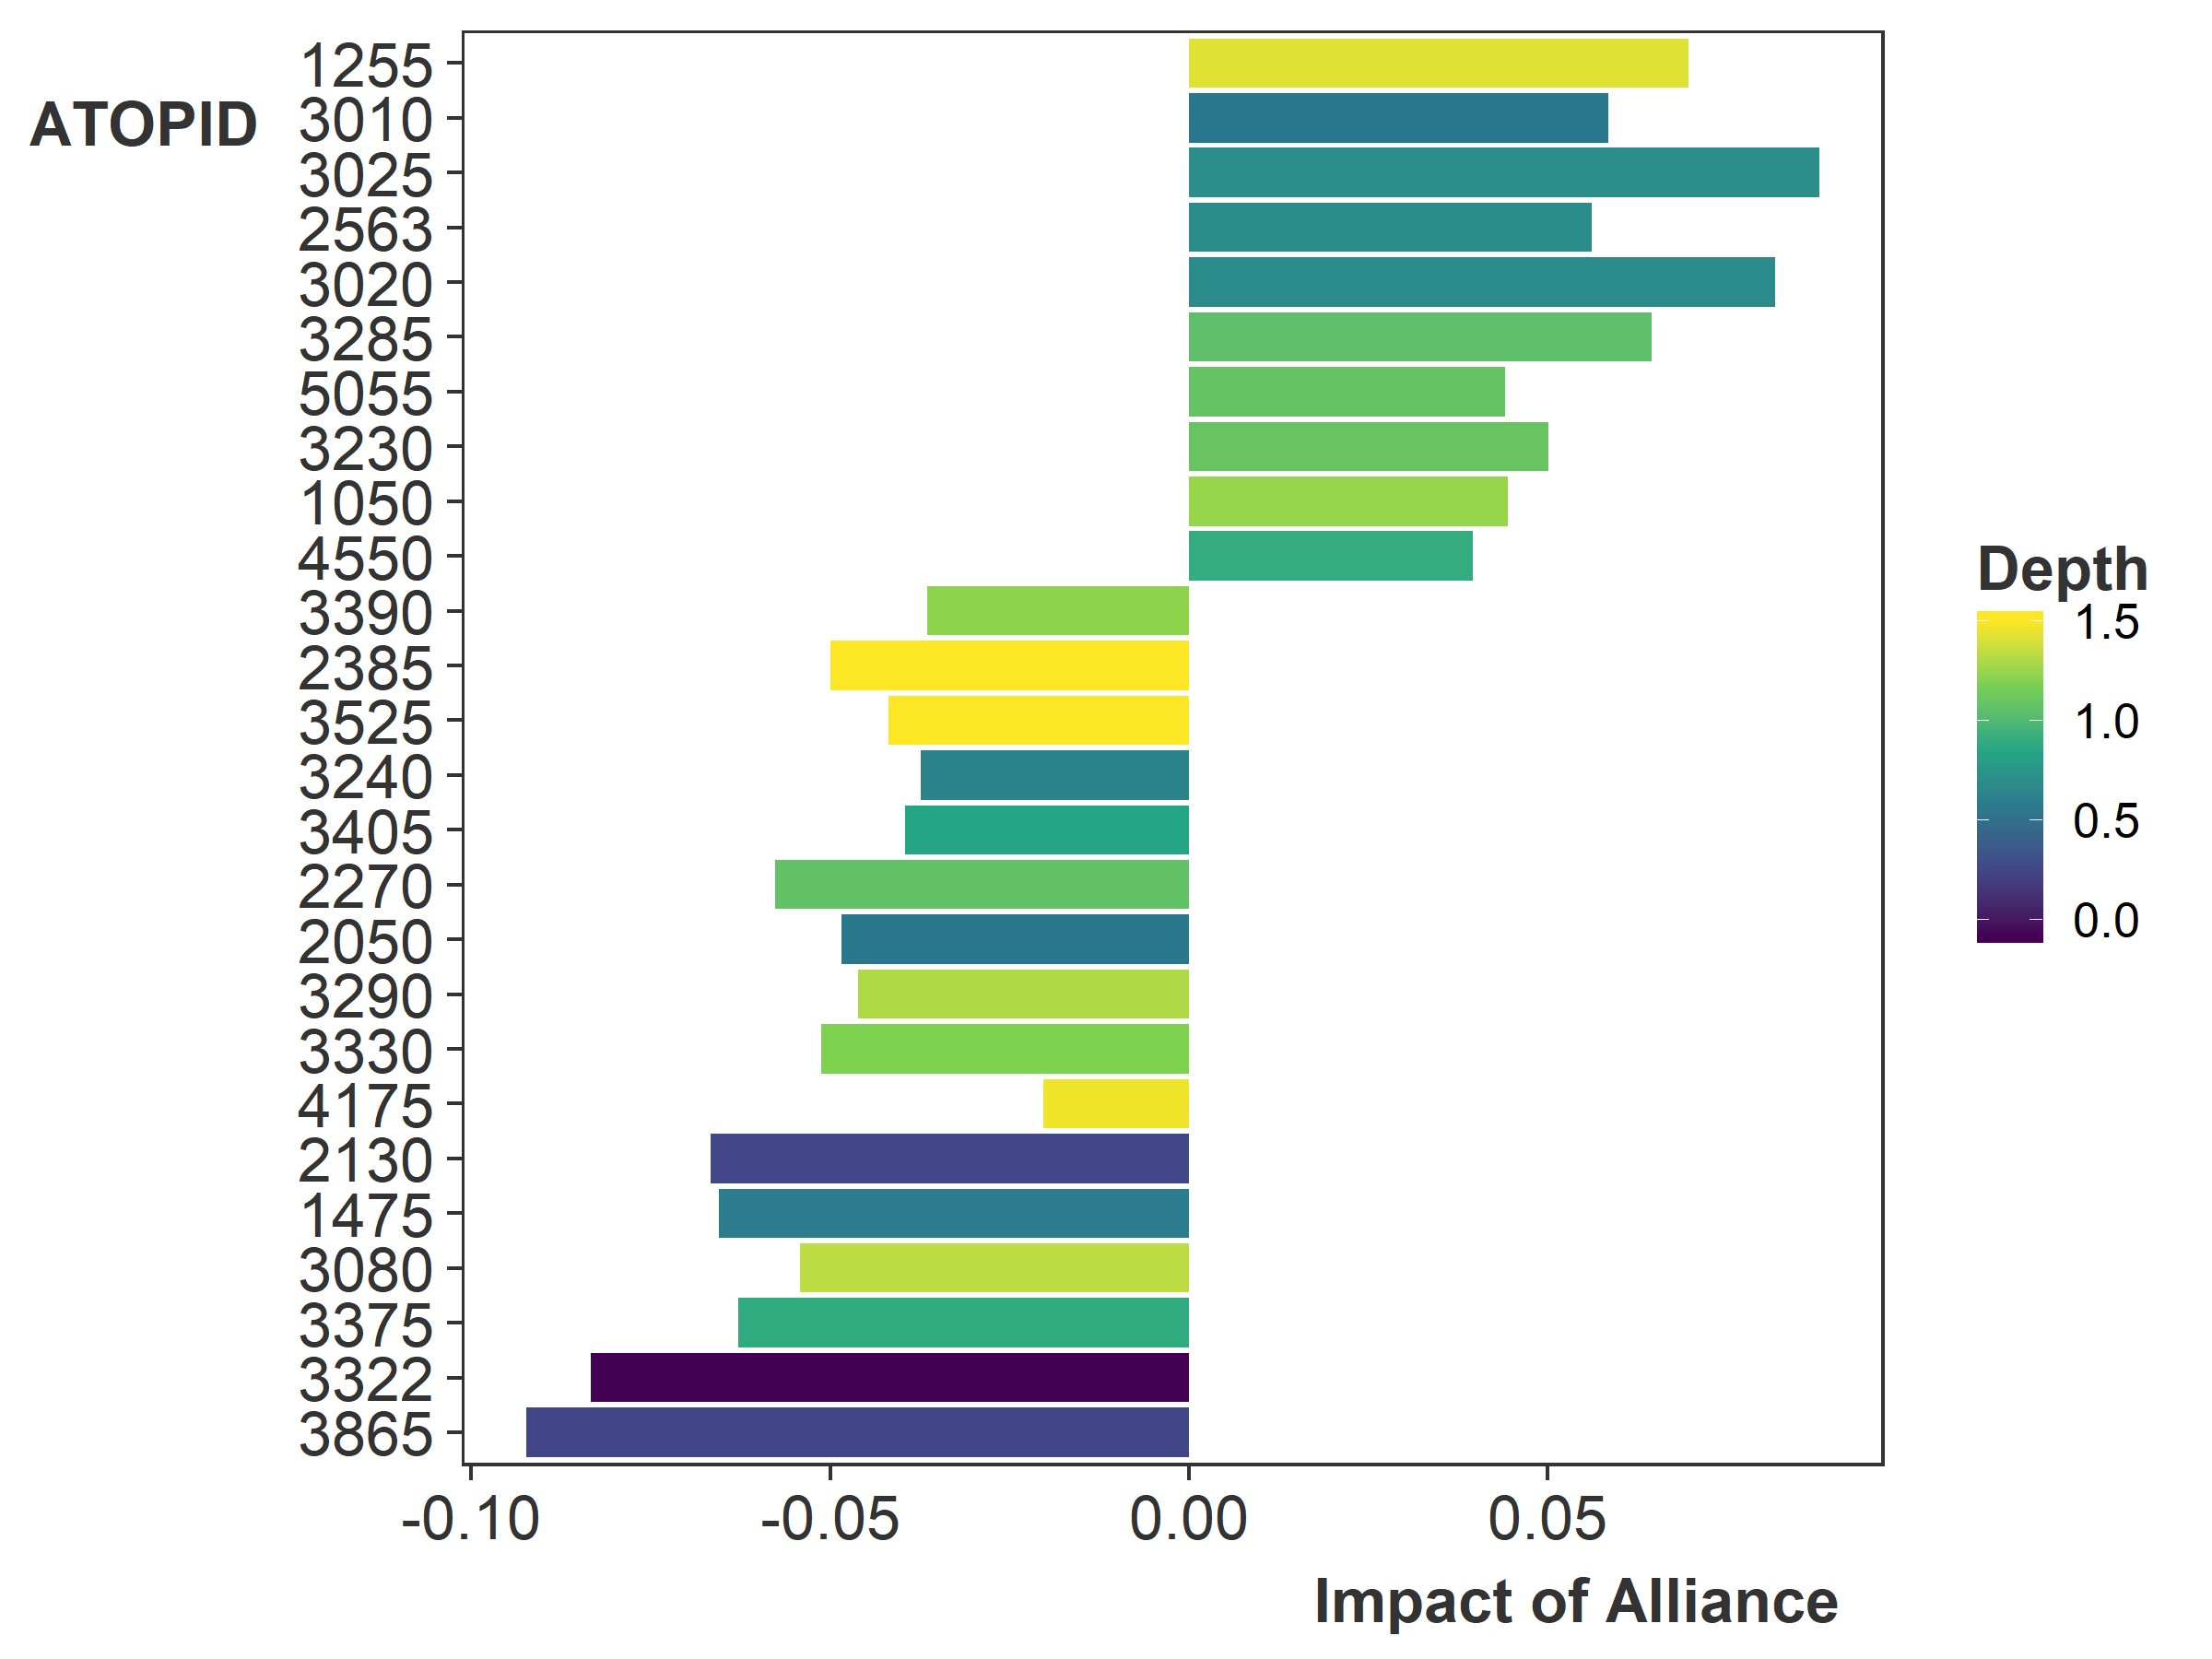
\includegraphics[width=0.95\textwidth]{non-zero-min.png}
	\label{fig:non-zero-min}
\end{figure}


\end{frame}


%------------------------------------------------

\begin{frame}{Impact of US Alliance on Non-major Power Military Spending} 

\begin{figure}
	\centering
		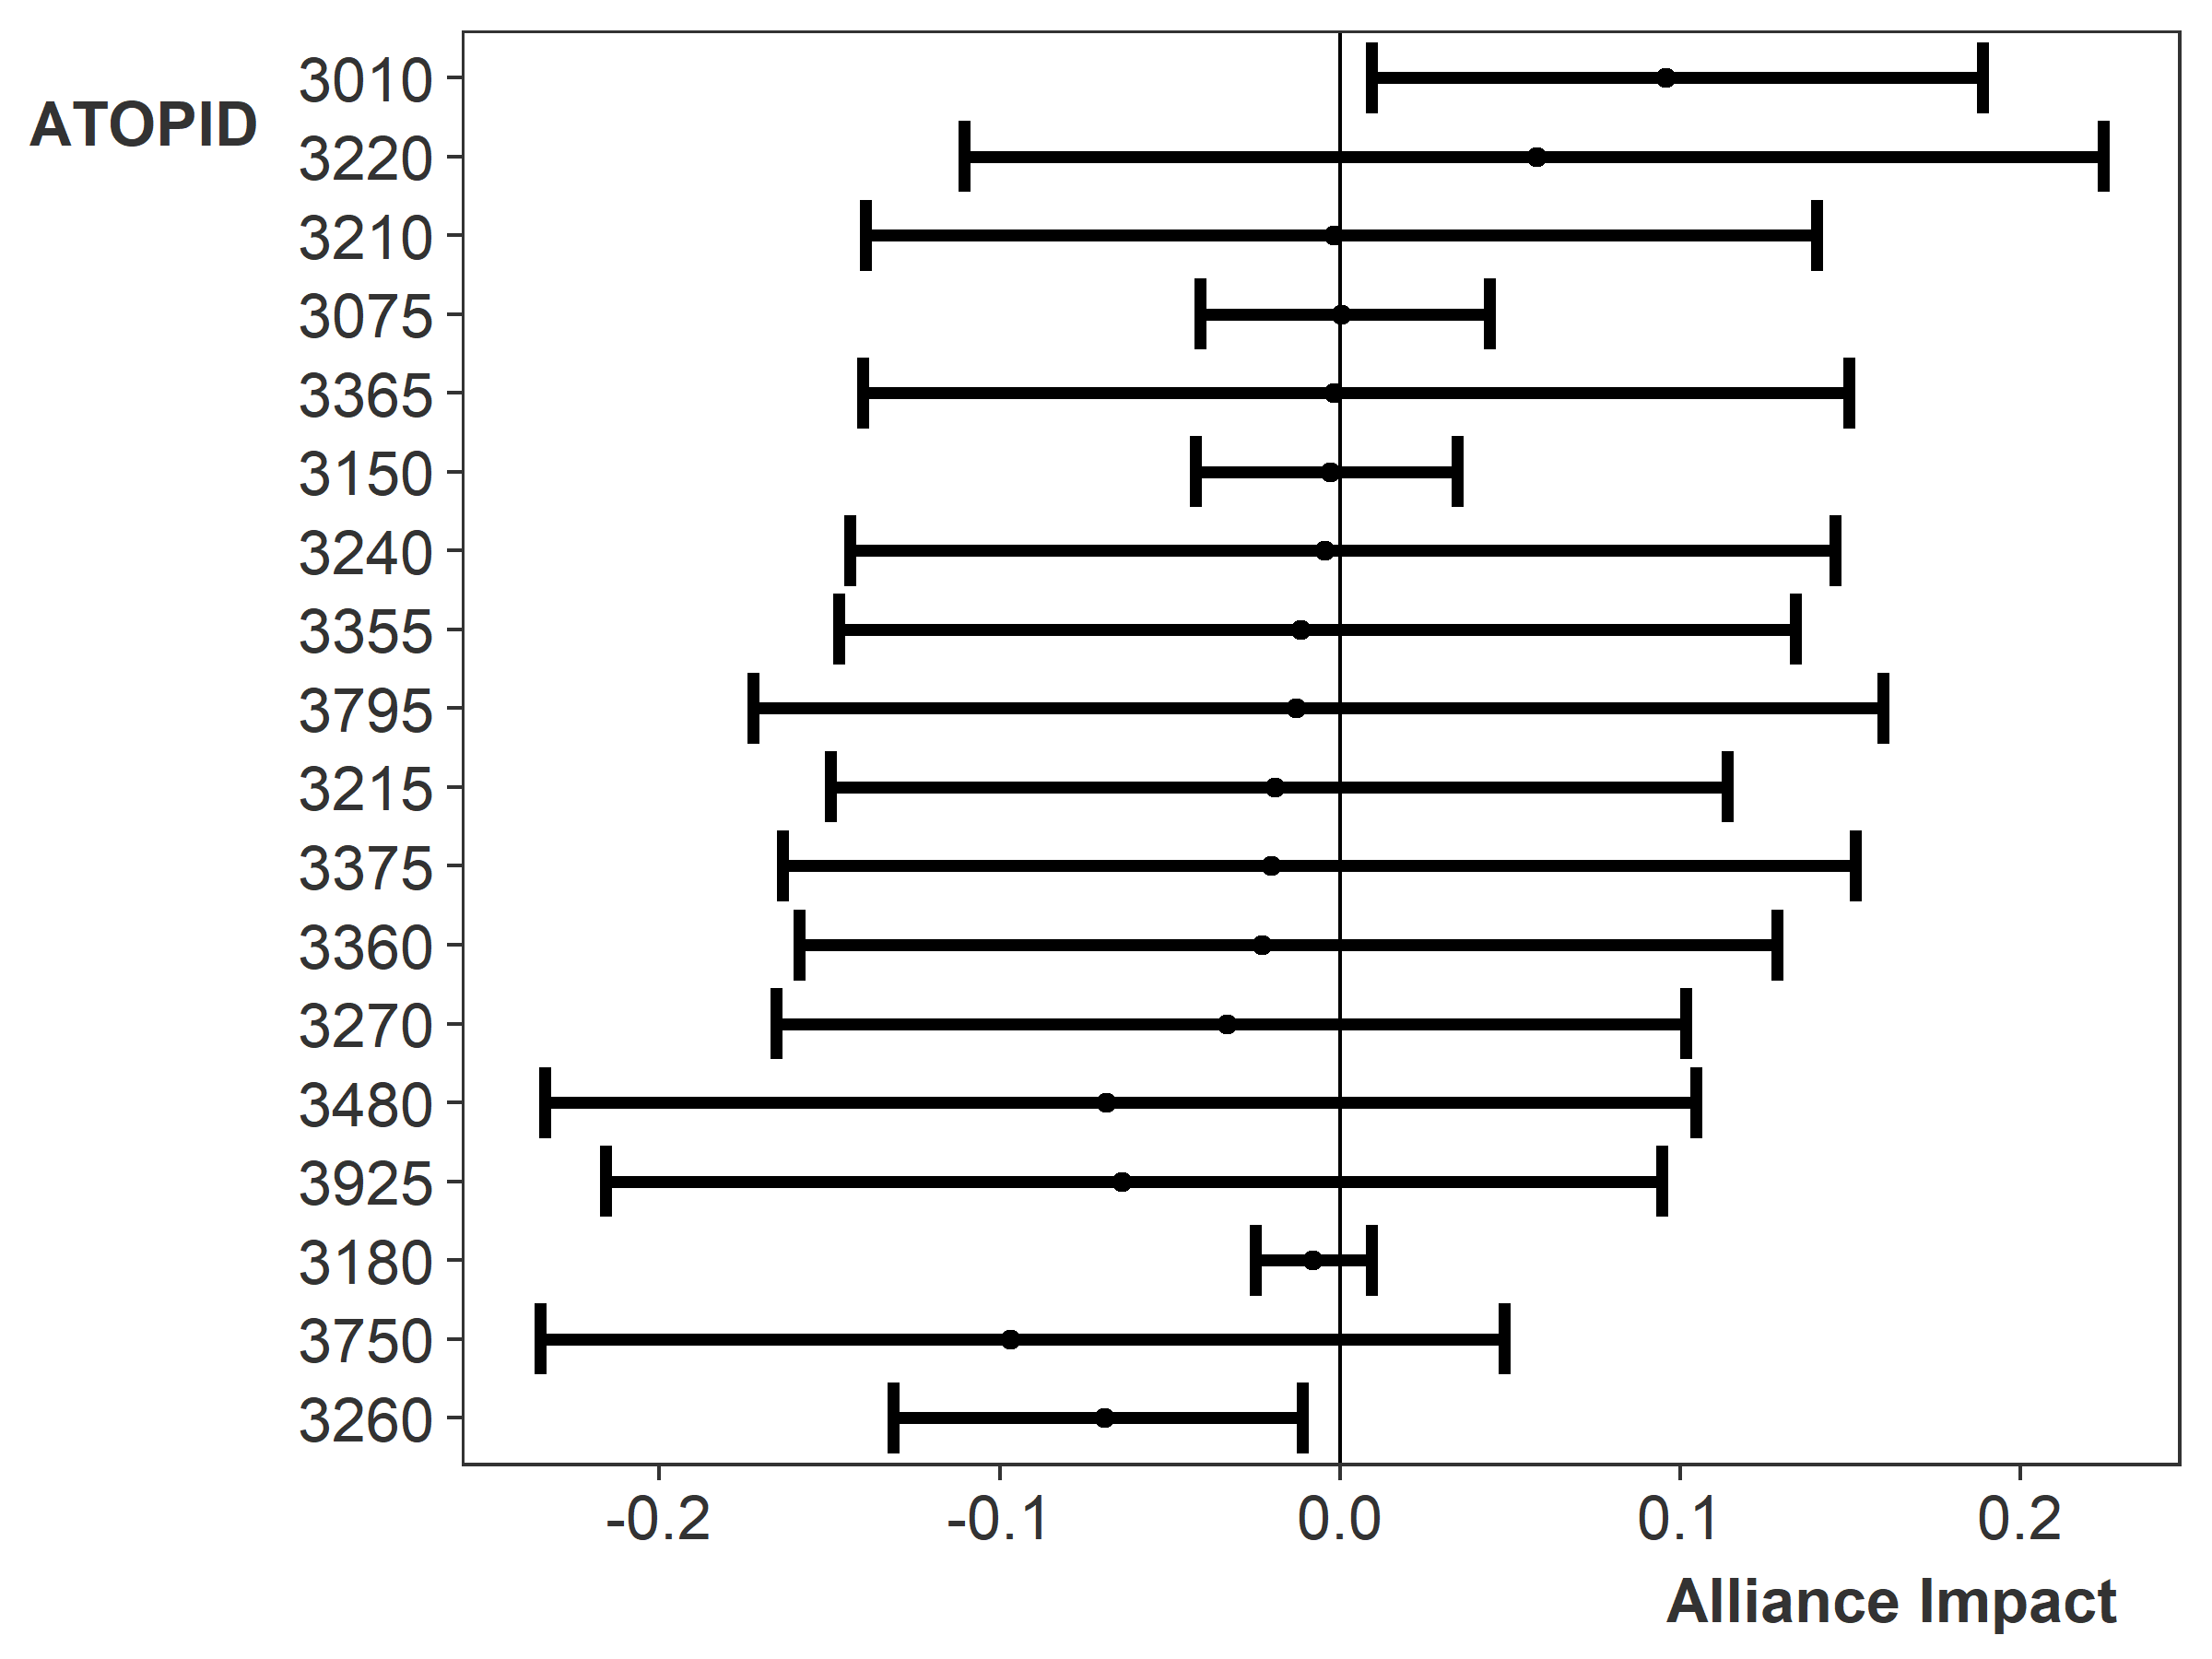
\includegraphics[width=0.85\textwidth]{lambda-us-min.png}
\end{figure}


\end{frame}

%------------------------------------------------

\begin{frame}{NATO} 

\begin{figure}
	\centering
		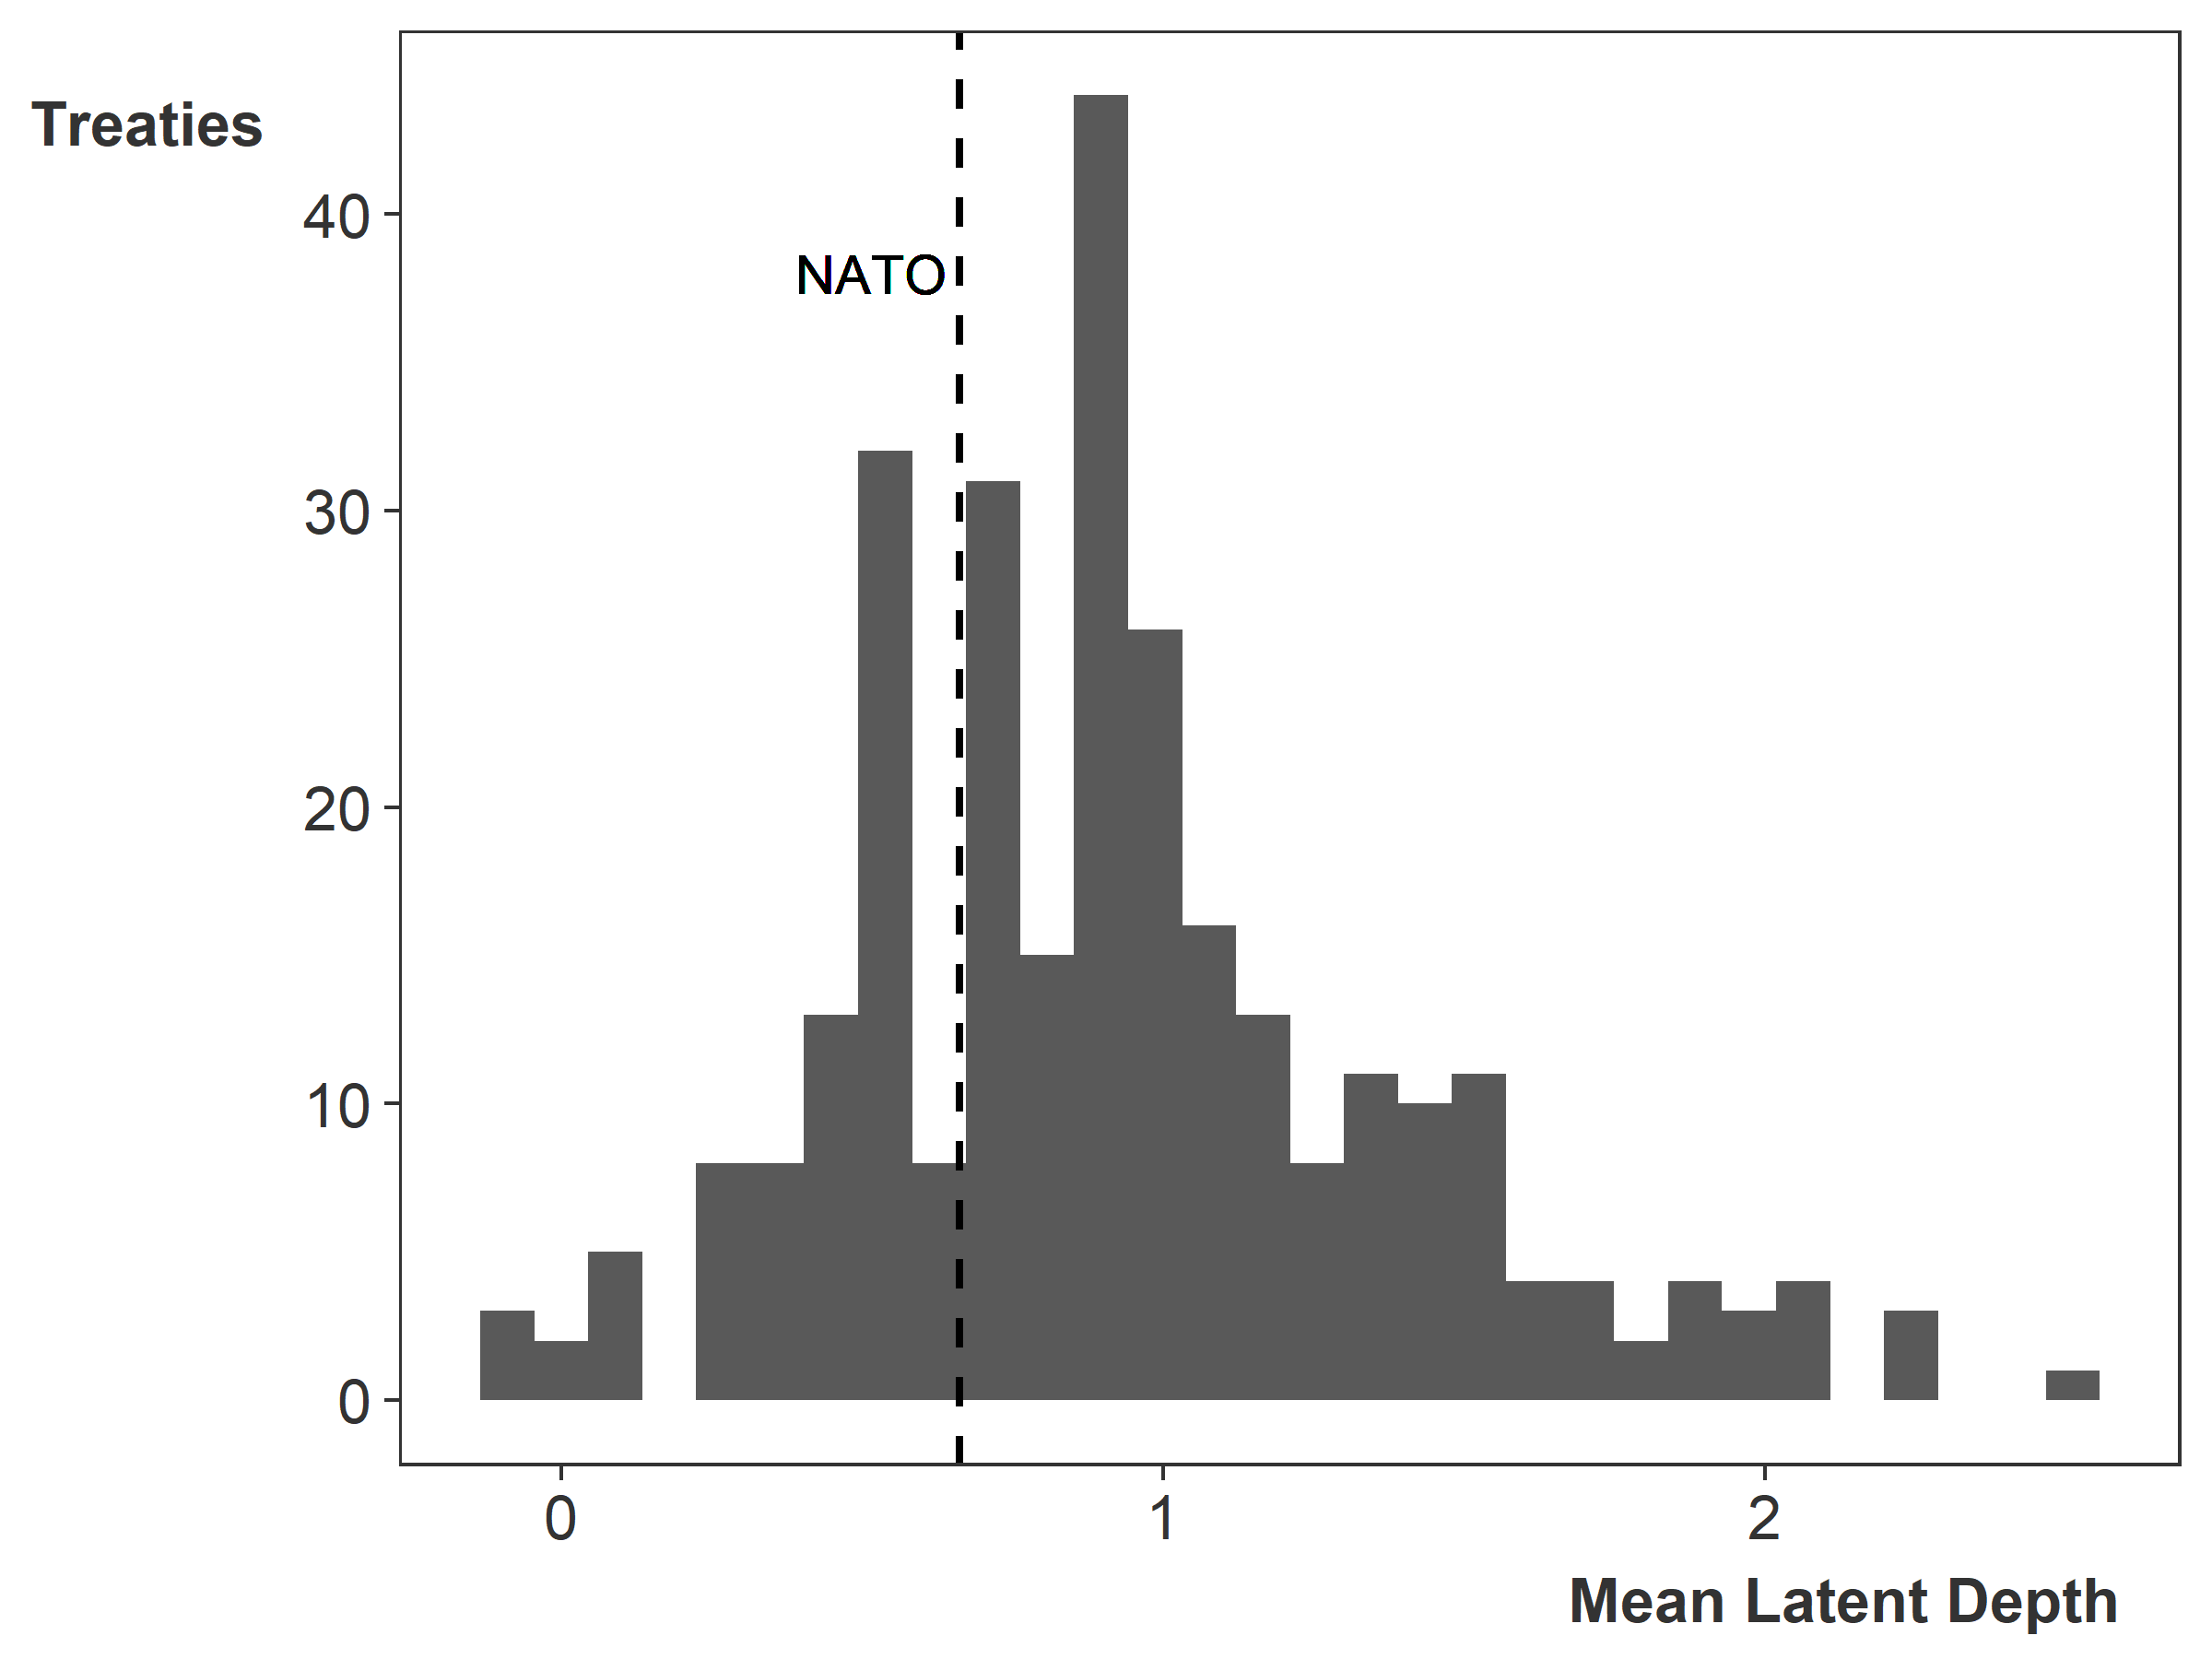
\includegraphics[width=0.95\textwidth]{ld-hist-nato.png}
\end{figure}


 \end{frame}


%%------------------------------------------------
%
%\begin{frame}{Alliance Participation and Military Spending: Belgium}
%
%
%\begin{figure}
%	\centering
%		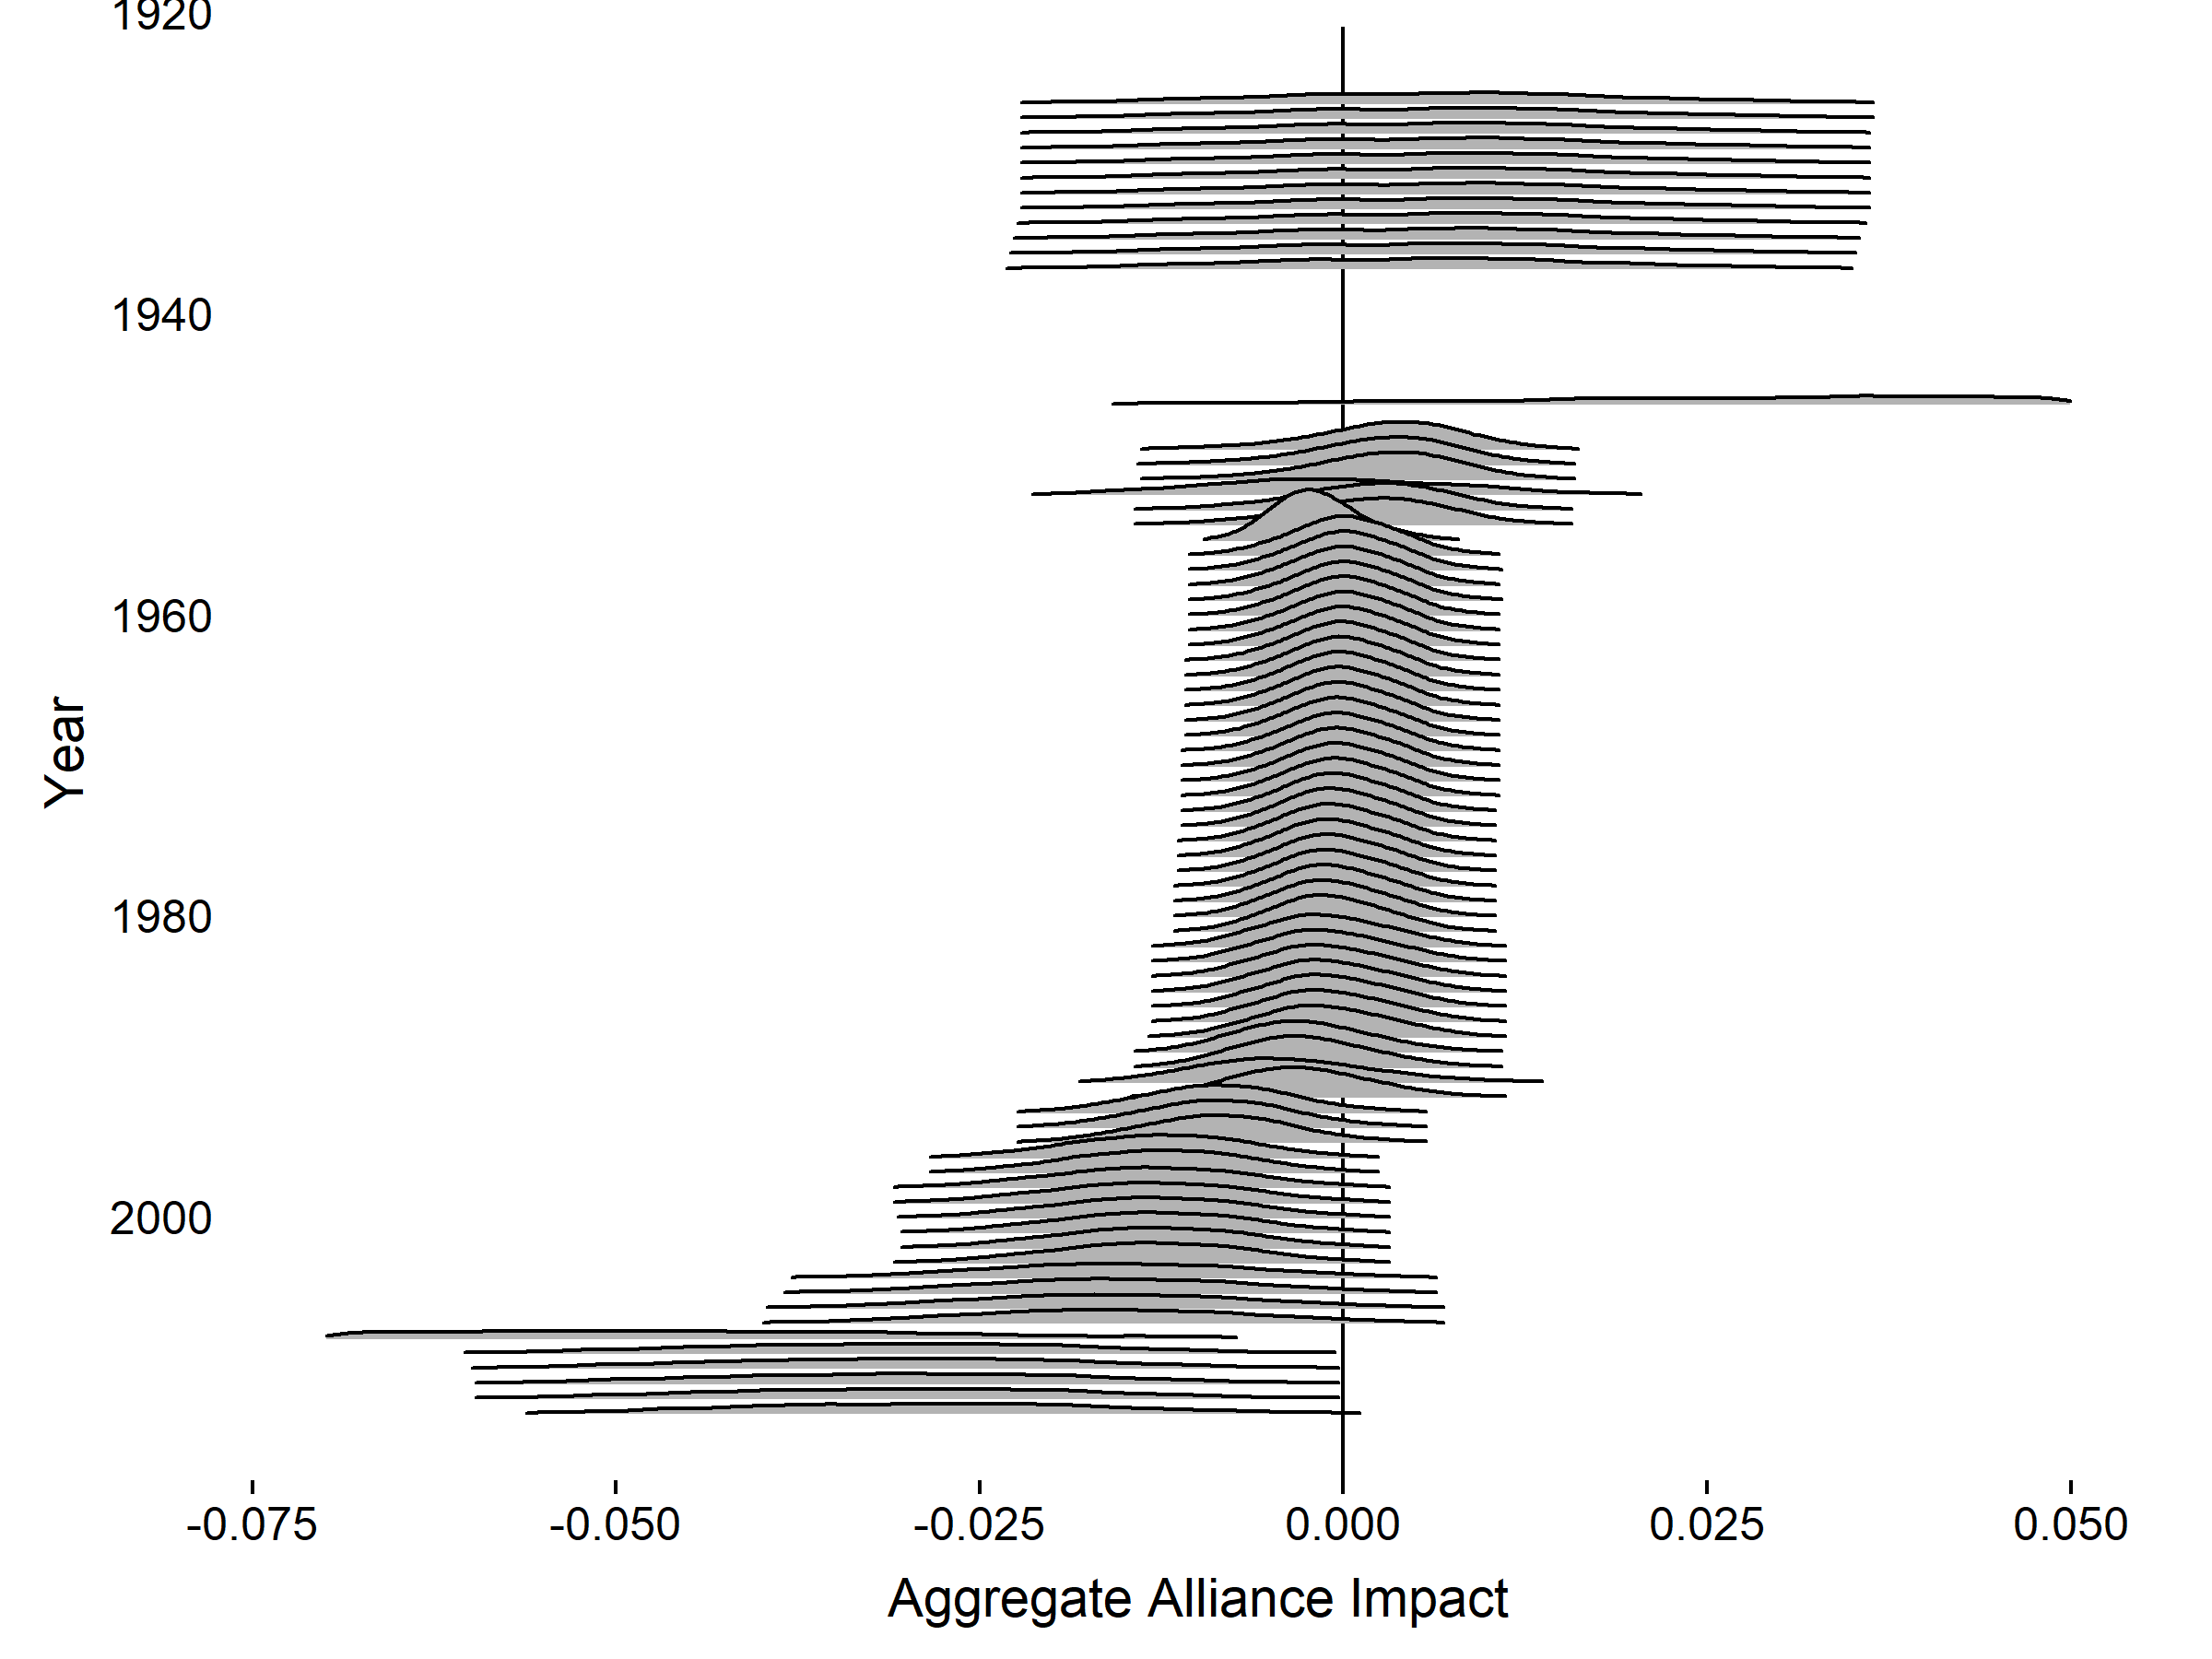
\includegraphics[width=0.95\textwidth]{bel-agg-imp.png}
%\end{figure}
%
%
%\end{frame}
%
%
%%------------------------------------------------
%
%\begin{frame}{Impact of NATO on Belgium}
%
%
%\begin{figure}
%	\centering
%		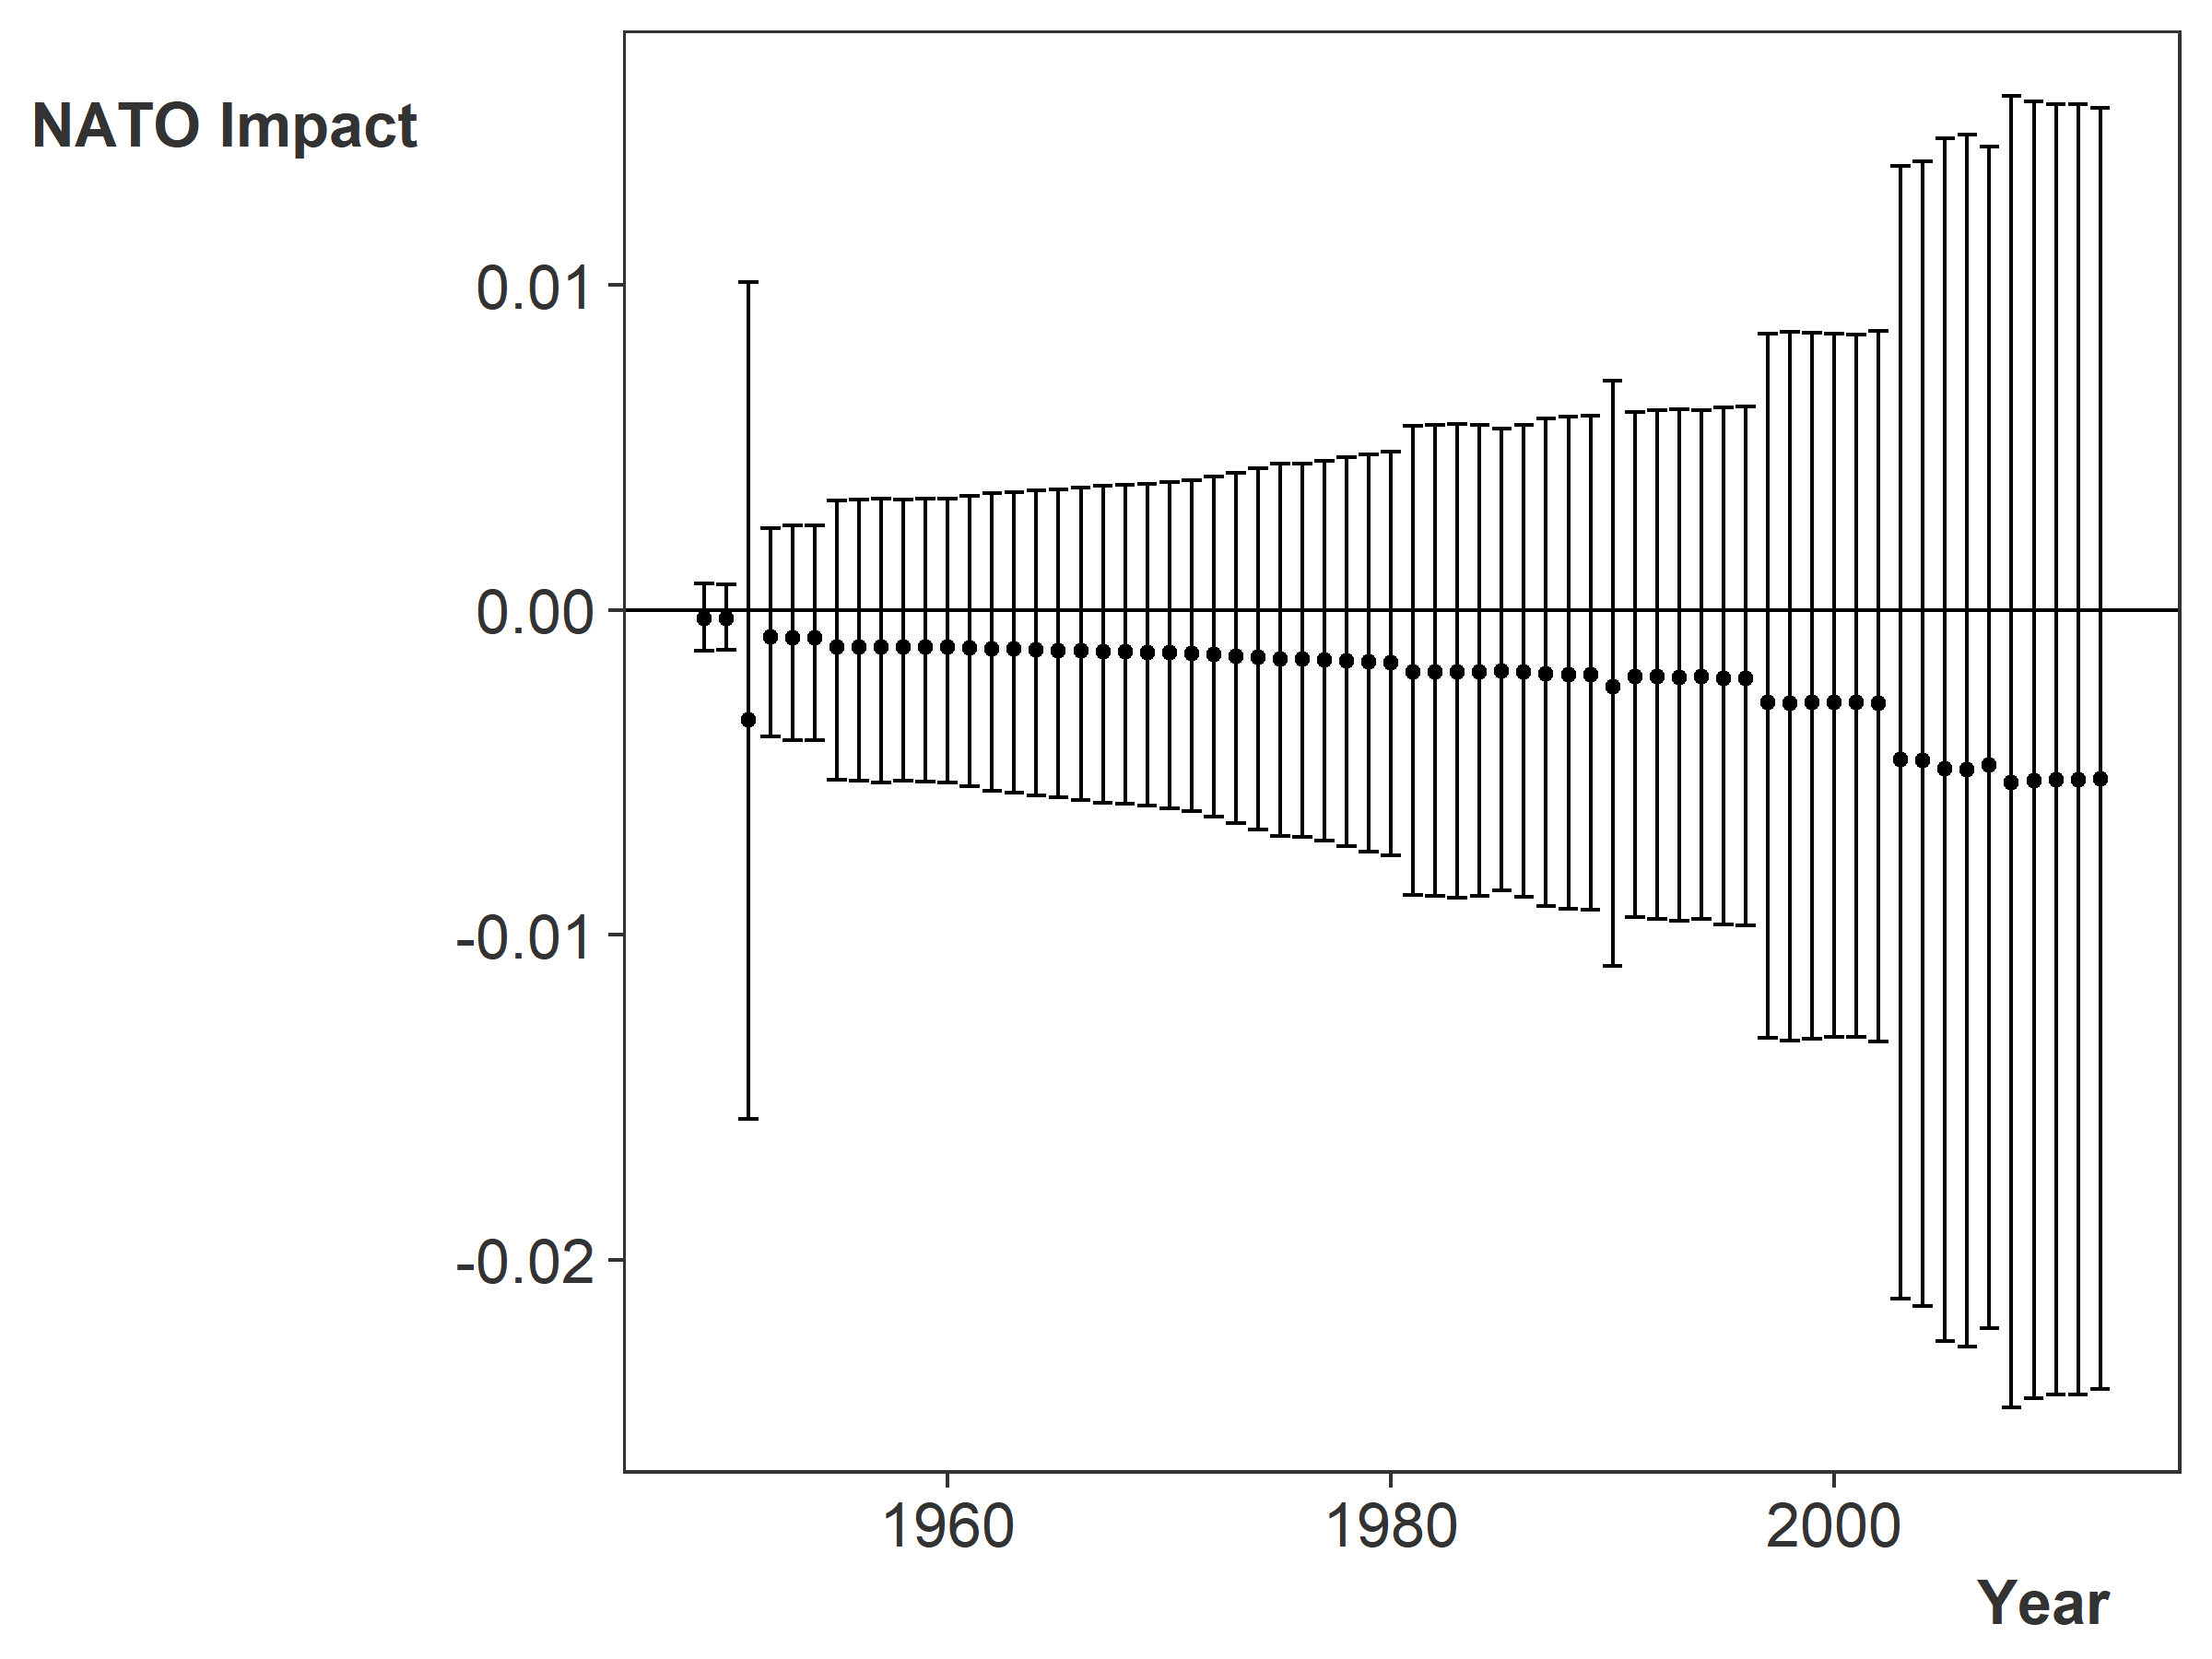
\includegraphics[width=0.95\textwidth]{bel-nato-imp.png}
%\end{figure}
%
%
%\end{frame}
%
%
%%------------------------------------------------
%
%\begin{frame}{Impact of EU on Belgium}
%
%
%\begin{figure}
%	\centering
%		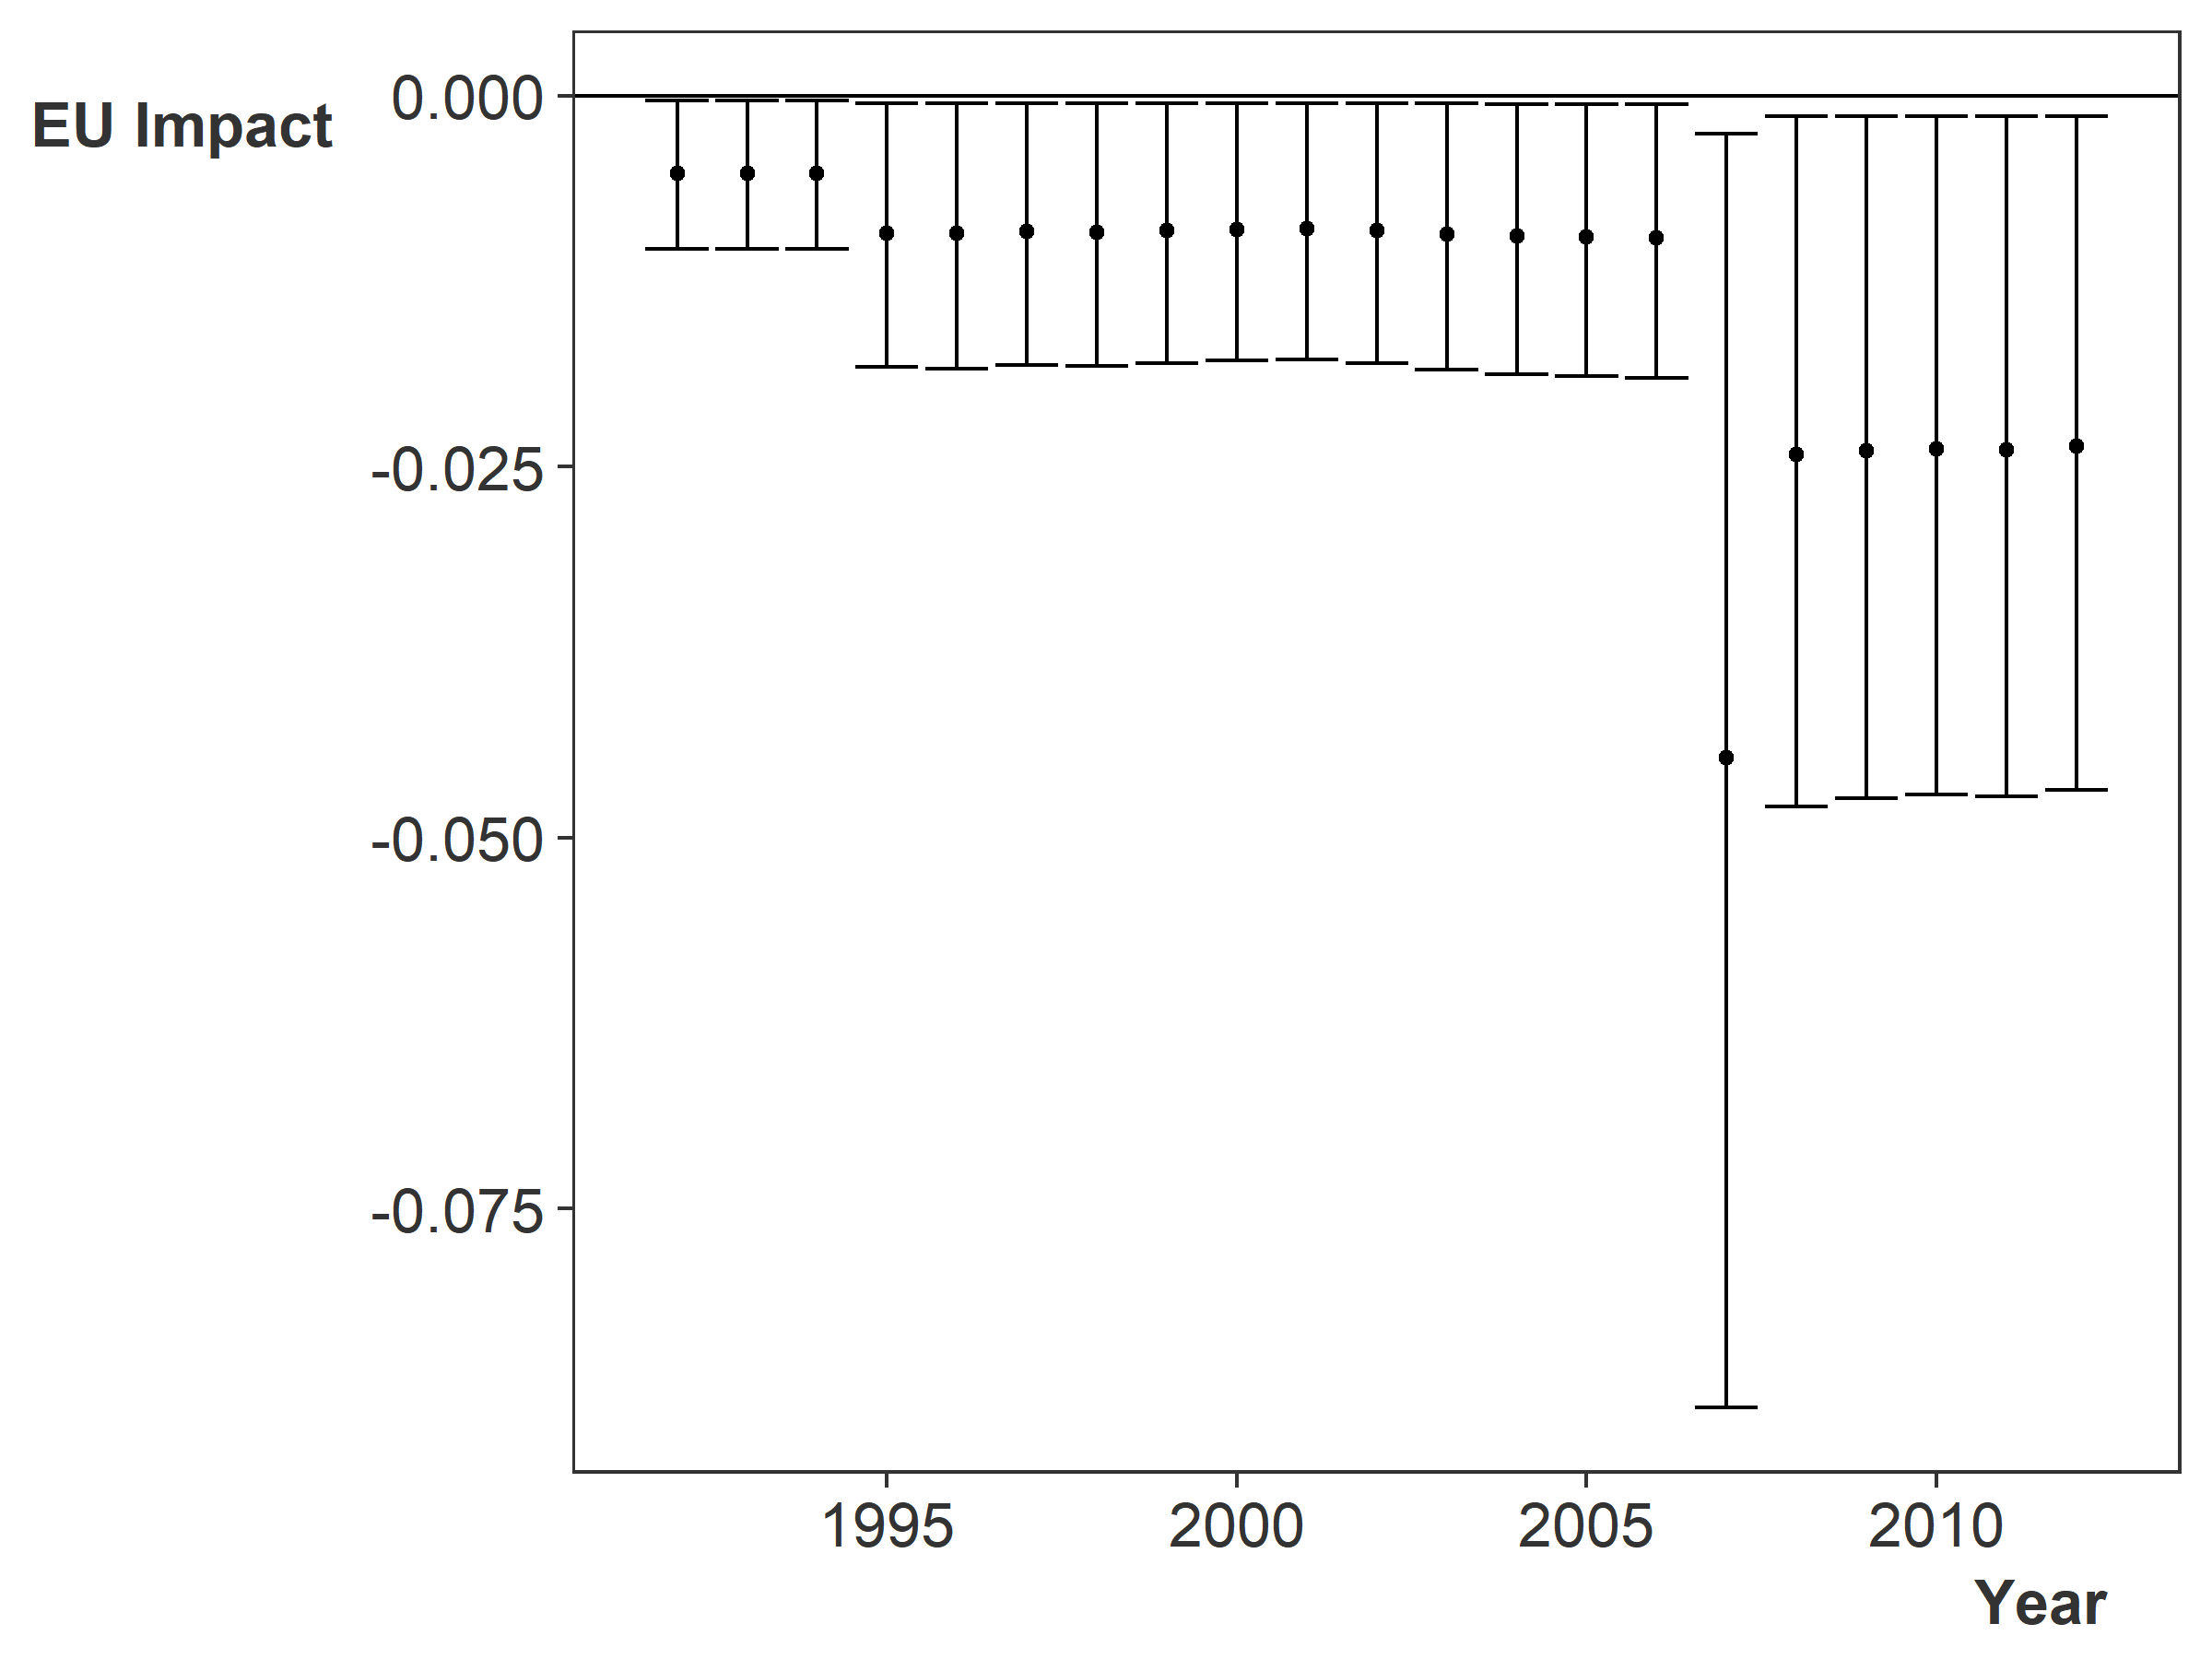
\includegraphics[width=0.95\textwidth]{bel-eu-imp.png}
%\end{figure}
%
%
%\end{frame}




%------------------------------------------------

\begin{frame}{Varying Slopes Model}

Within each of the $j$ groups of state capability, for $i$ in $1 ... n_j$: 
\begin{equation*}
y_i \sim student_t(\nu_j, \alpha_j + \alpha^{st} + \alpha^{yr} +\textbf{W}_{i} \gamma  + \textbf{Z}_{ji} \lambda_{j}, \sigma_j) 
\end{equation*} 

\begin{equation*}
\lambda_{j} \sim N(\theta_{j}, \sigma^{all}_{j})
\end{equation*} 

\begin{equation*}
\theta_{j} = \alpha^{all}_{j} + \textbf{X} \beta_j
\end{equation*}

I give $\beta_j$ a multivariate normal prior with prior scale $\tau$:
\begin{equation*}
\beta_j \sim MVN(\mu_{\beta_j}, \Sigma_{\beta}) 
\end{equation*}

\end{frame}


%------------------------------------------------

\begin{frame}{Varying Slopes Results: Depth}

\begin{figure}[htbp]
	\centering
		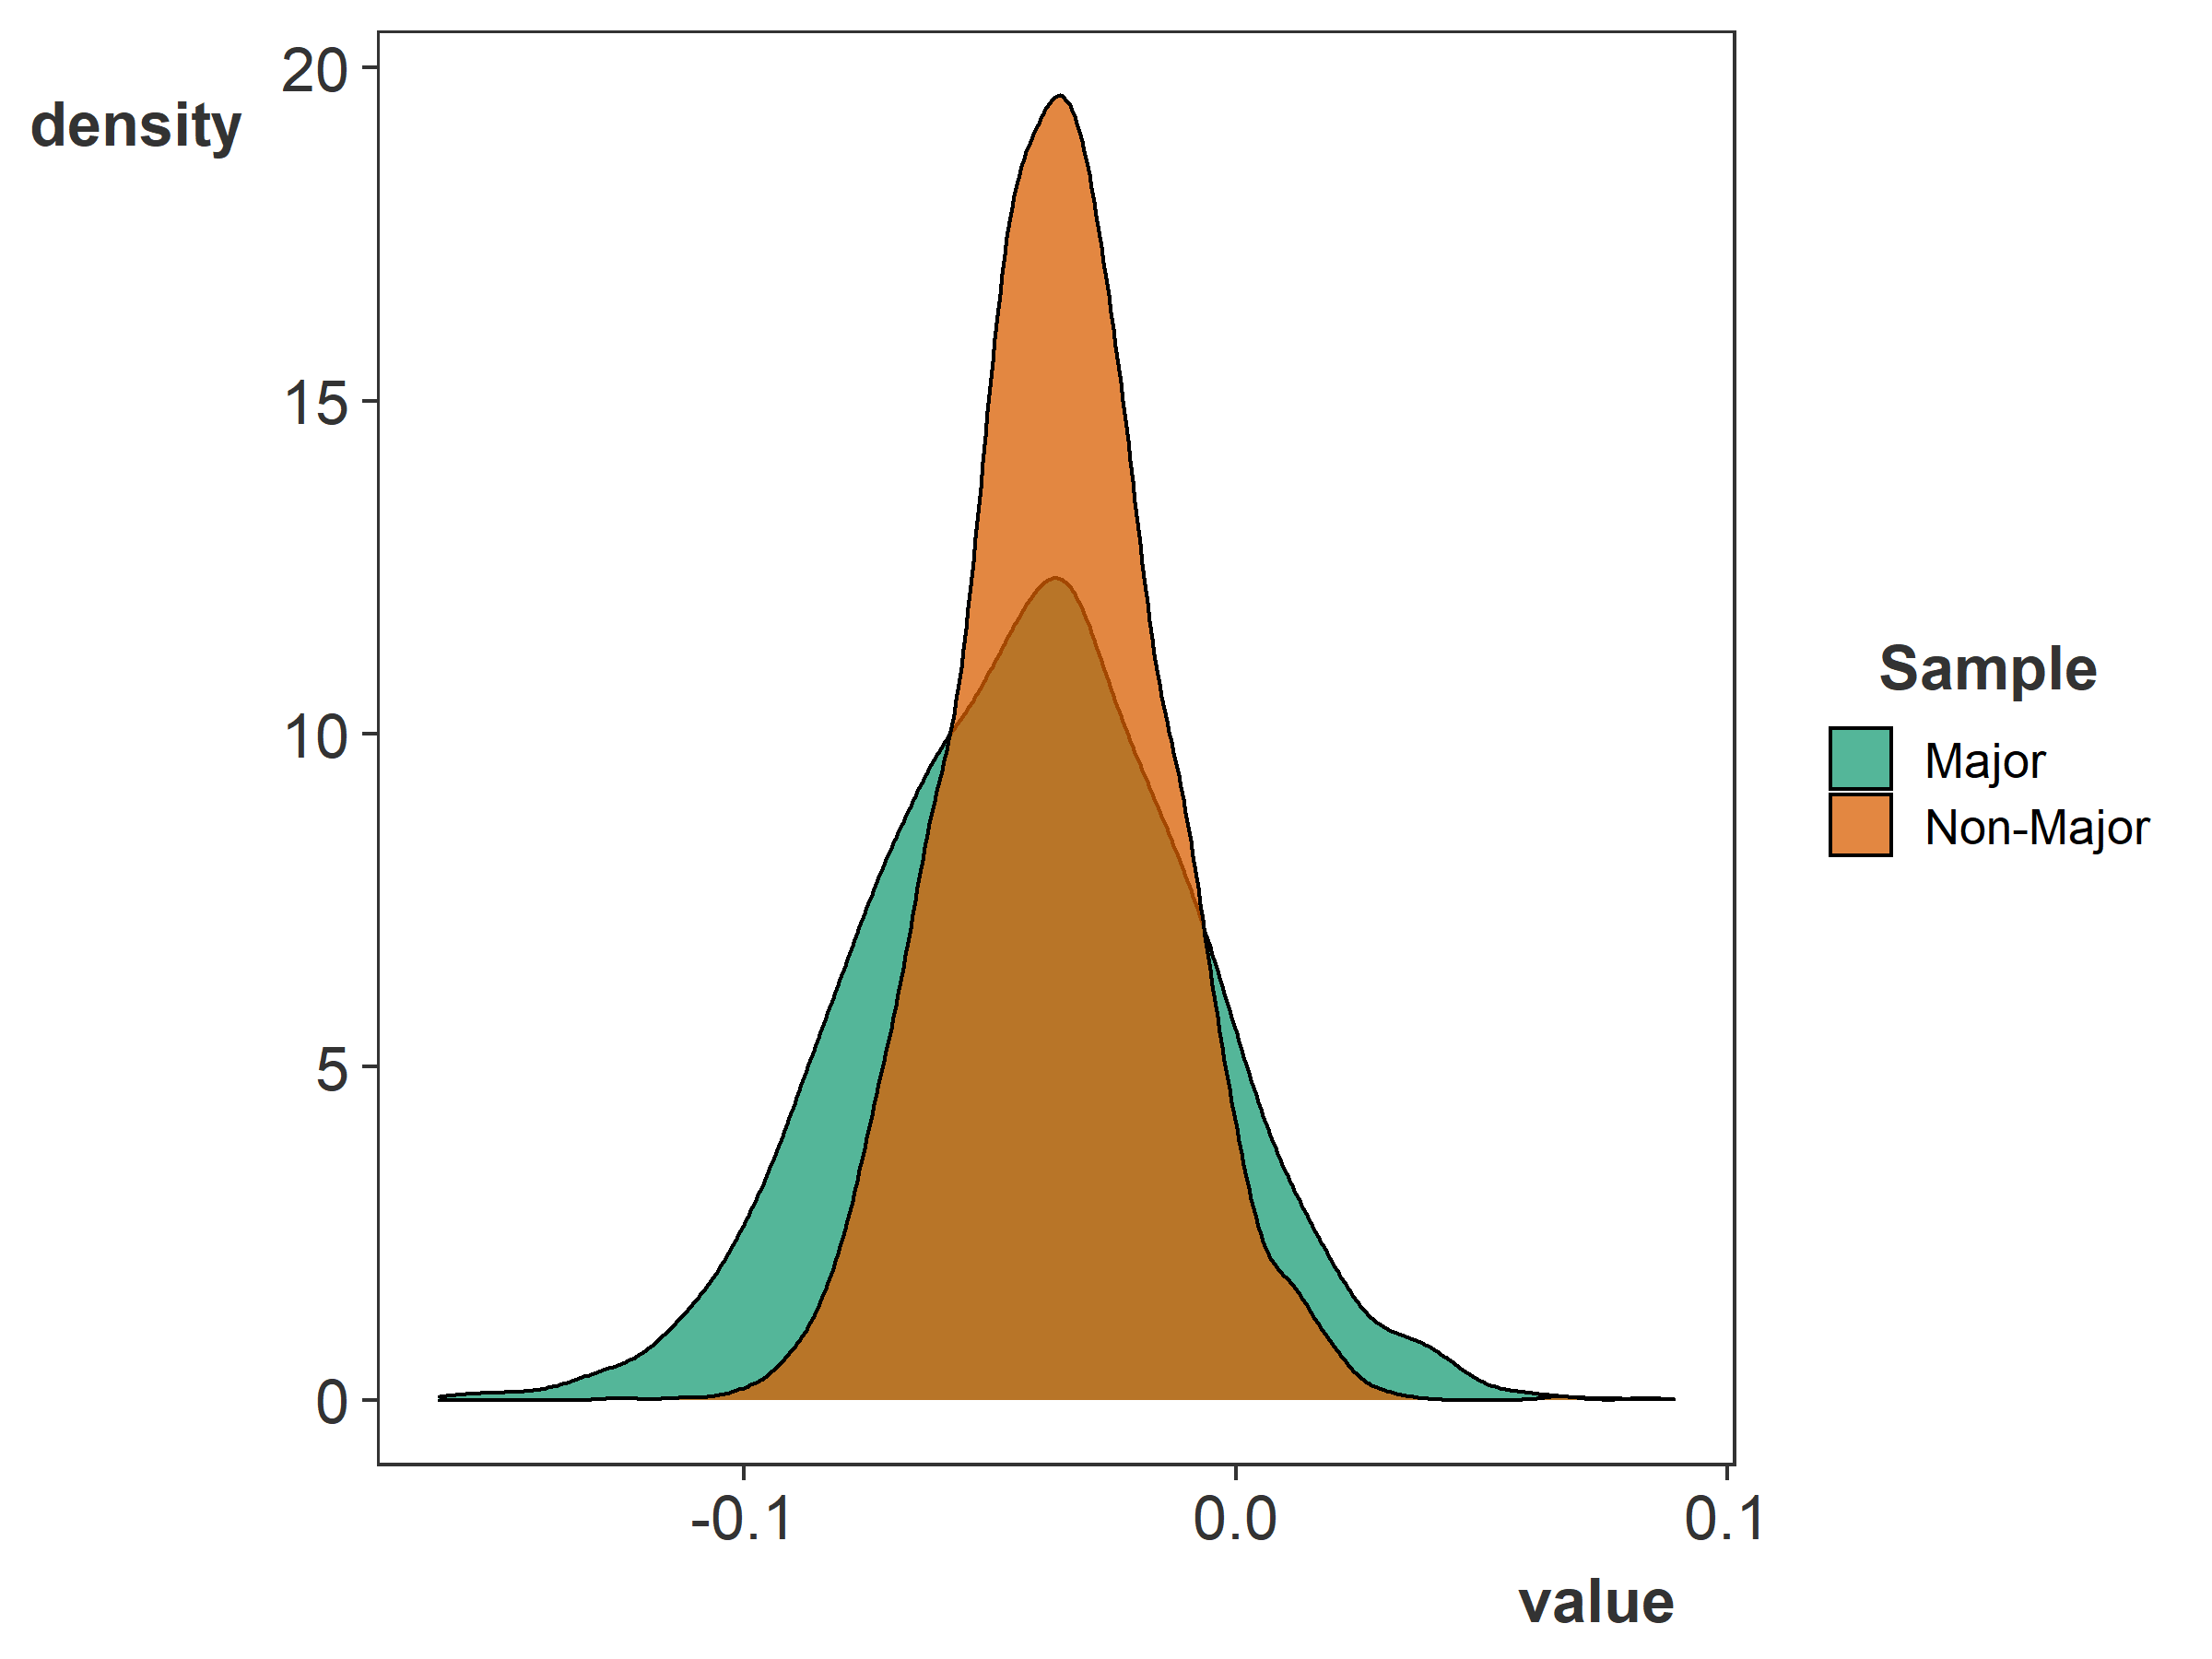
\includegraphics[width=0.95\textwidth]{var-slopes-depth.png}
\end{figure}

\end{frame}


%------------------------------------------------

\begin{frame}{Treaty depth and $\lambda$: Major Powers}

\begin{figure}
	\centering
		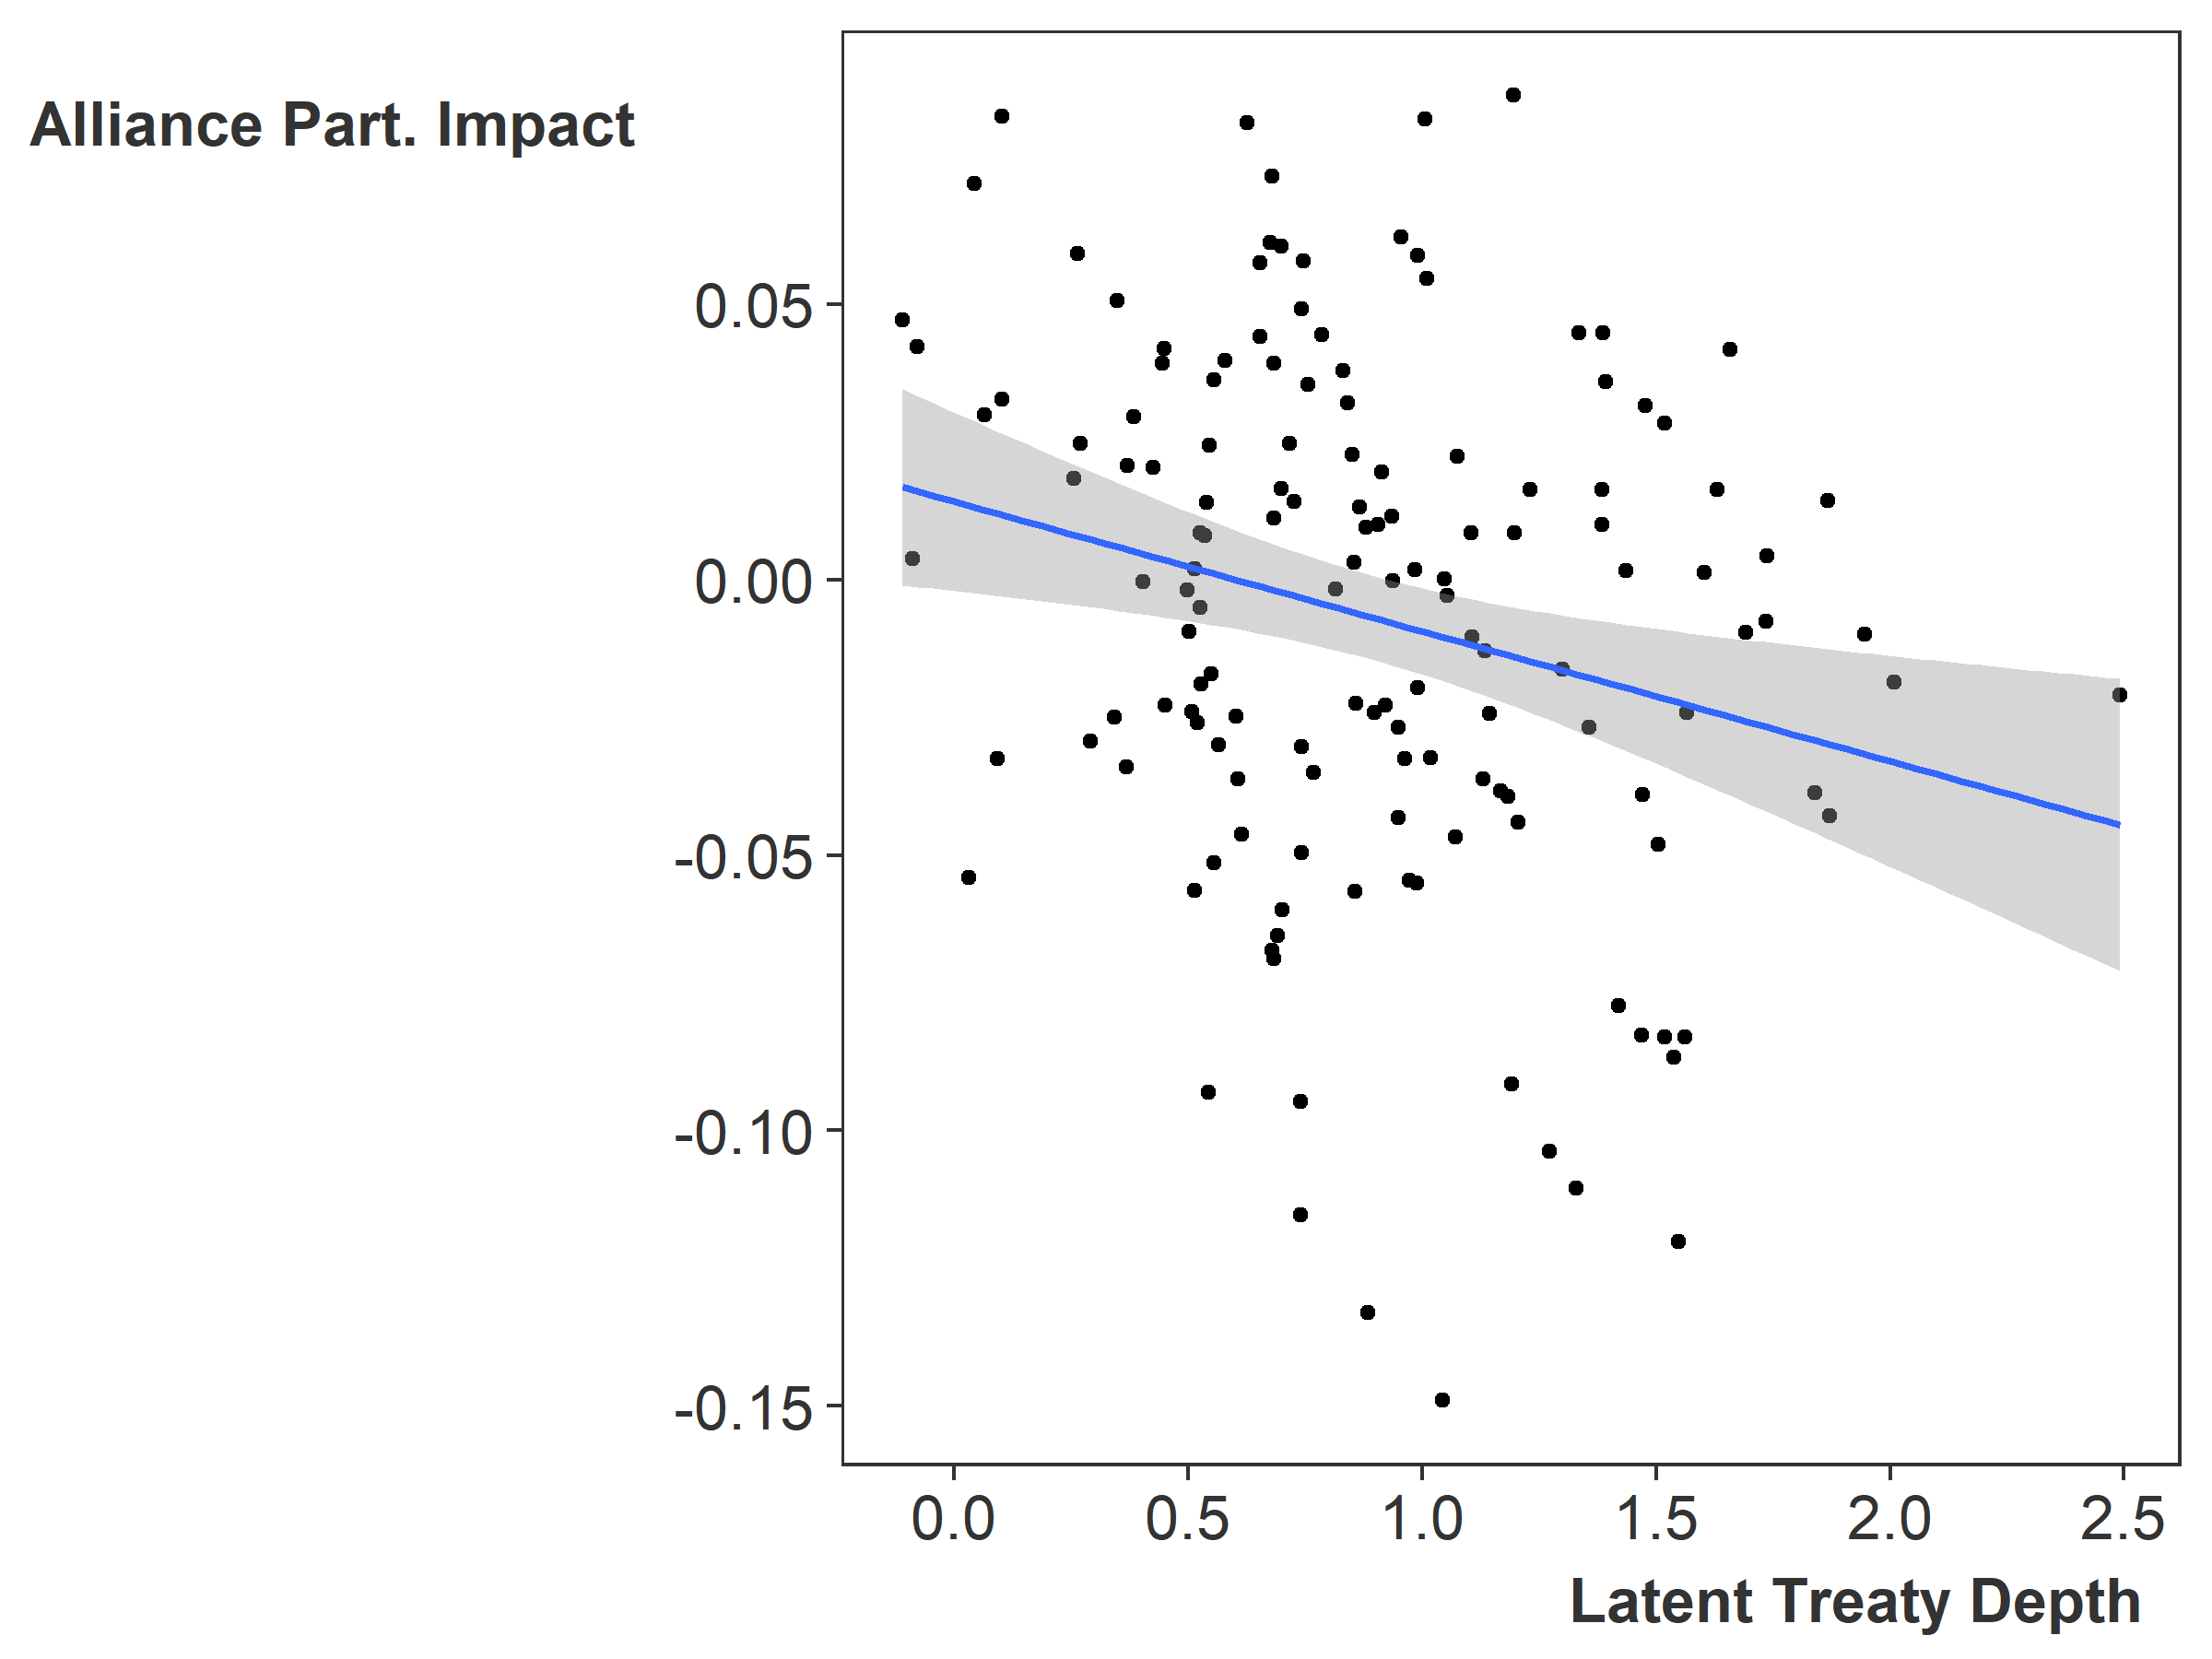
\includegraphics[width=0.95\textwidth]{ld-lambda-maj.png}
	\label{fig:ls-lambda-min}
\end{figure}


\end{frame}

%------------------------------------------------

\begin{frame}{Full Varying Slopes Results}

\begin{figure}[htbp]
	\centering
		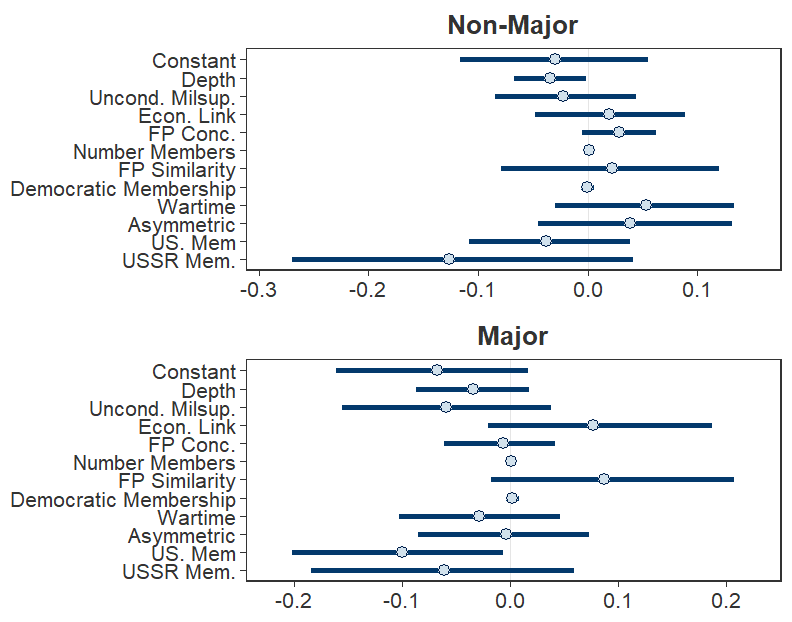
\includegraphics[width=0.95\textwidth]{vs-res-full.png}
\end{figure}

\end{frame}

%------------------------------------------------

\begin{frame}{Impact of Alliances on US}


\begin{figure}
	\centering
		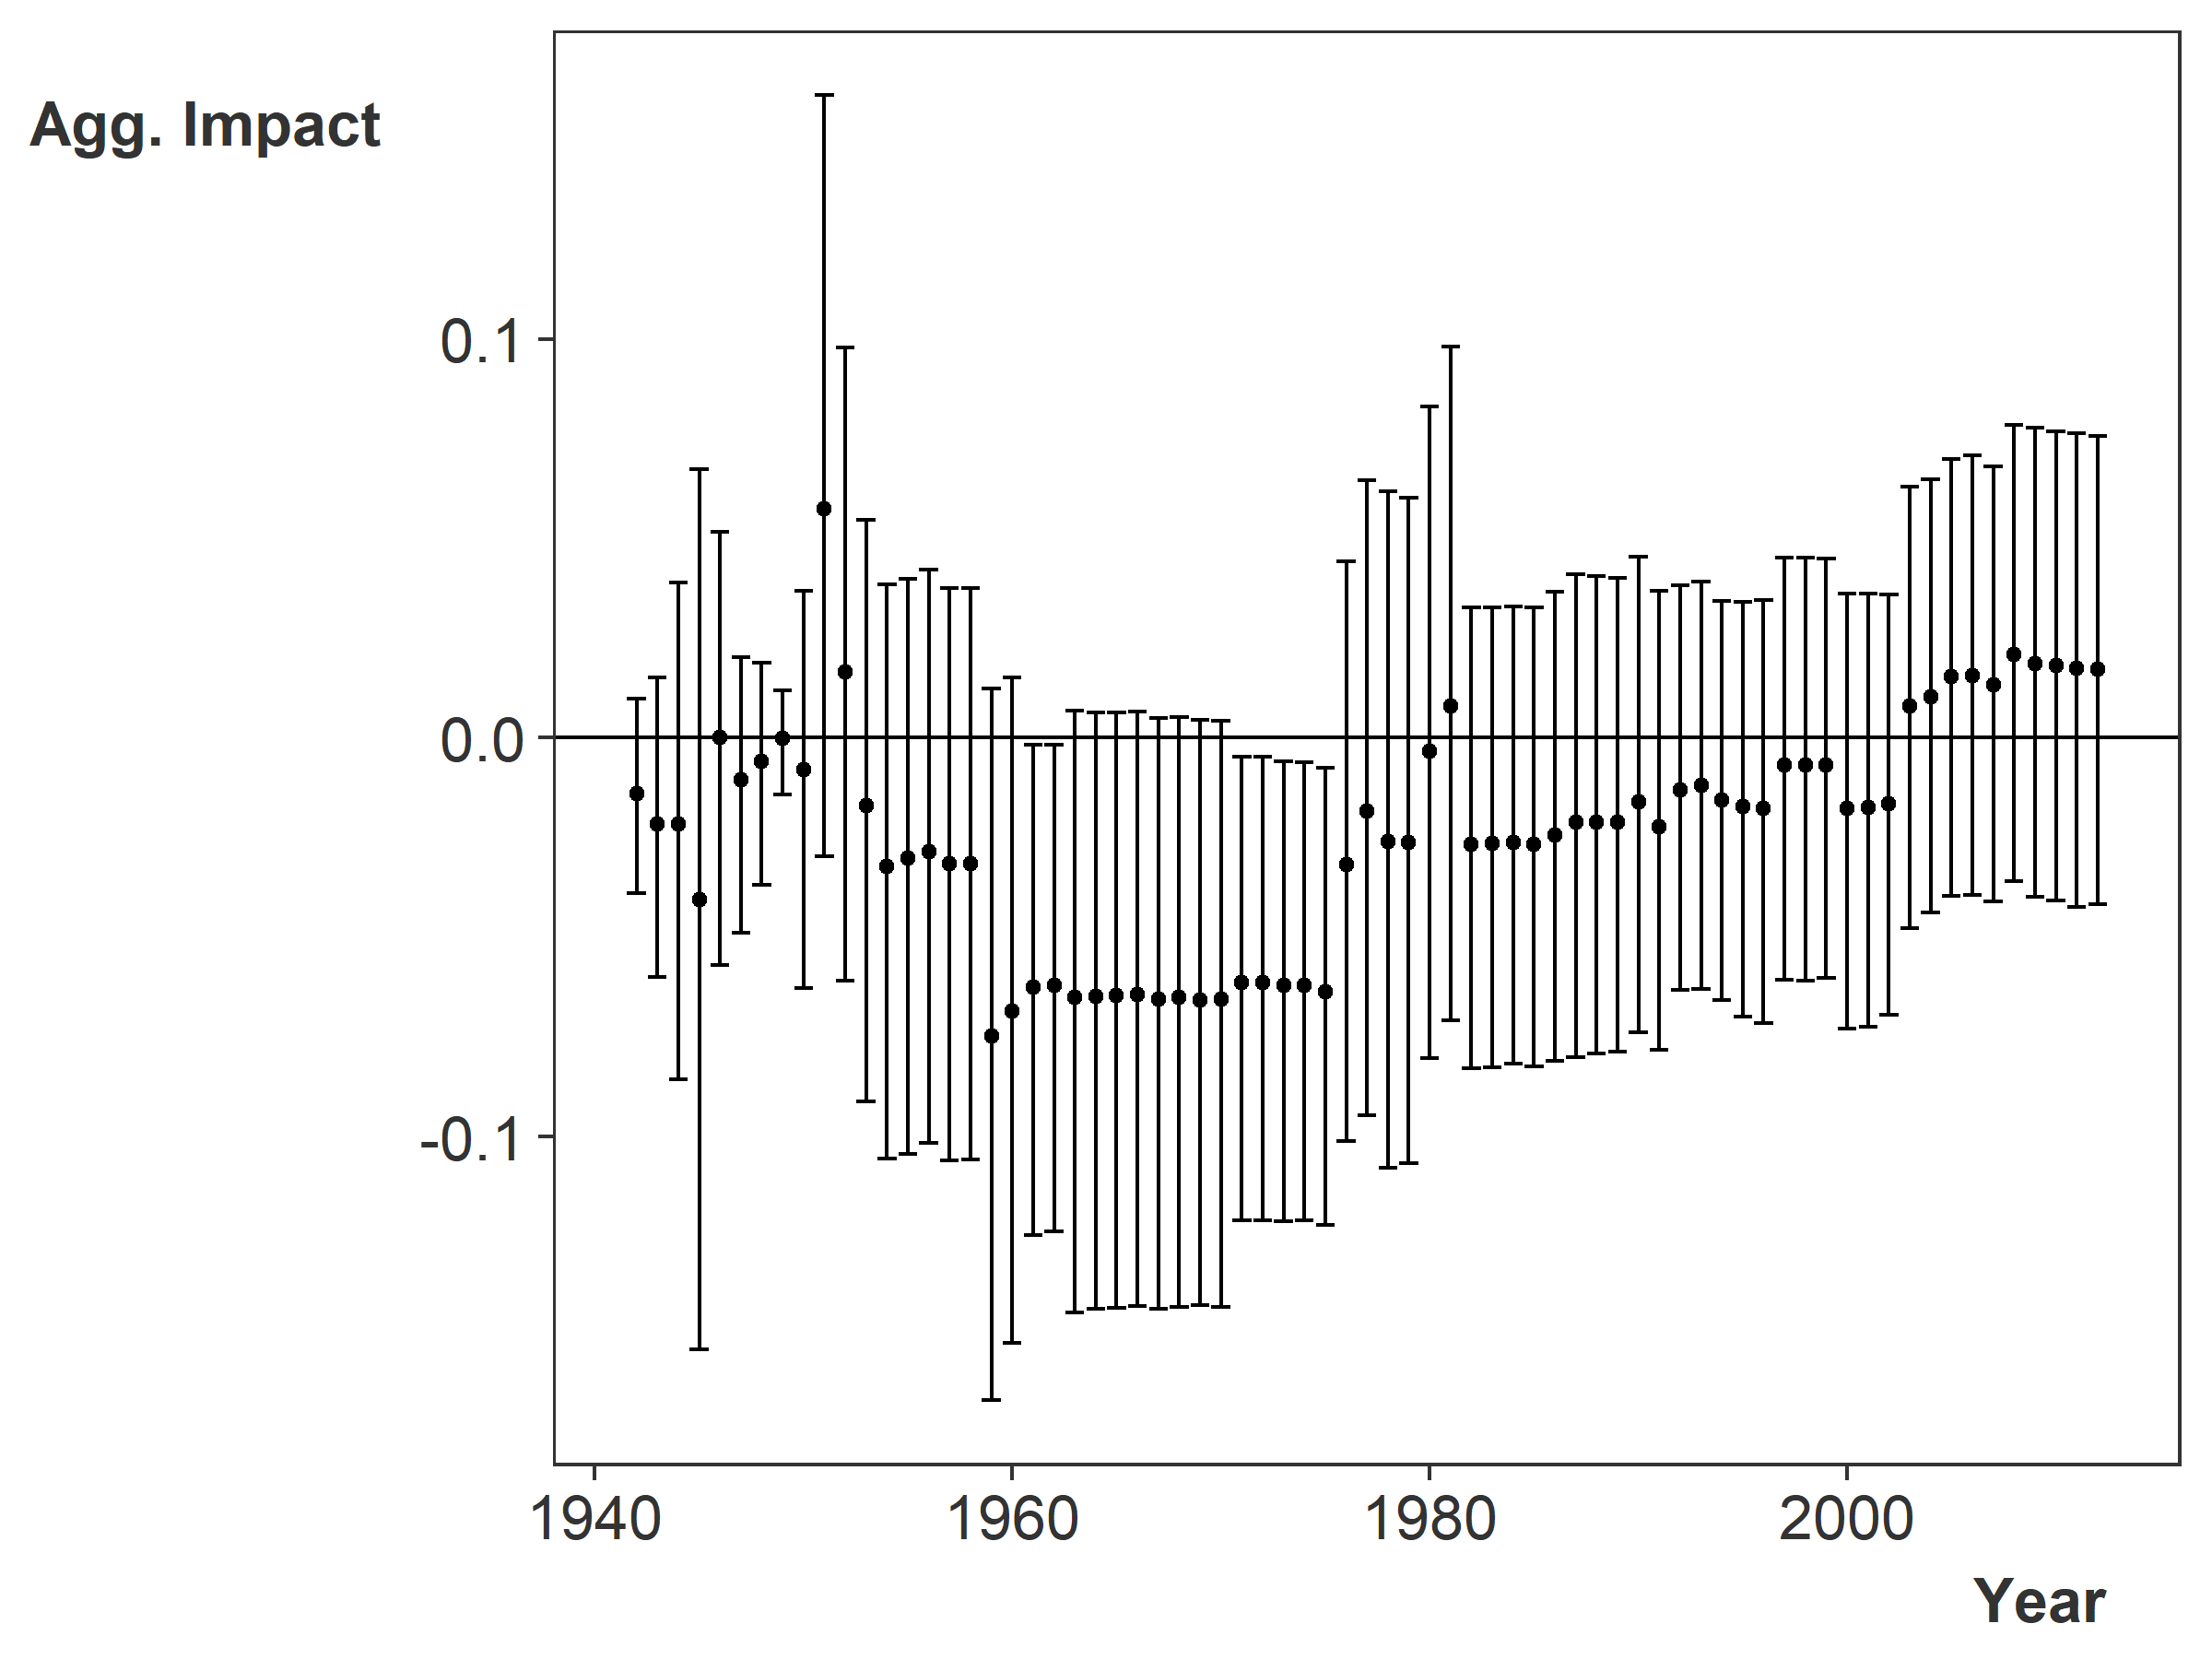
\includegraphics[width=0.95\textwidth]{us-agg-imp.png}
\end{figure}


\end{frame}

%------------------------------------------------

\begin{frame}{Impact of NATO on US}


\begin{figure}
	\centering
		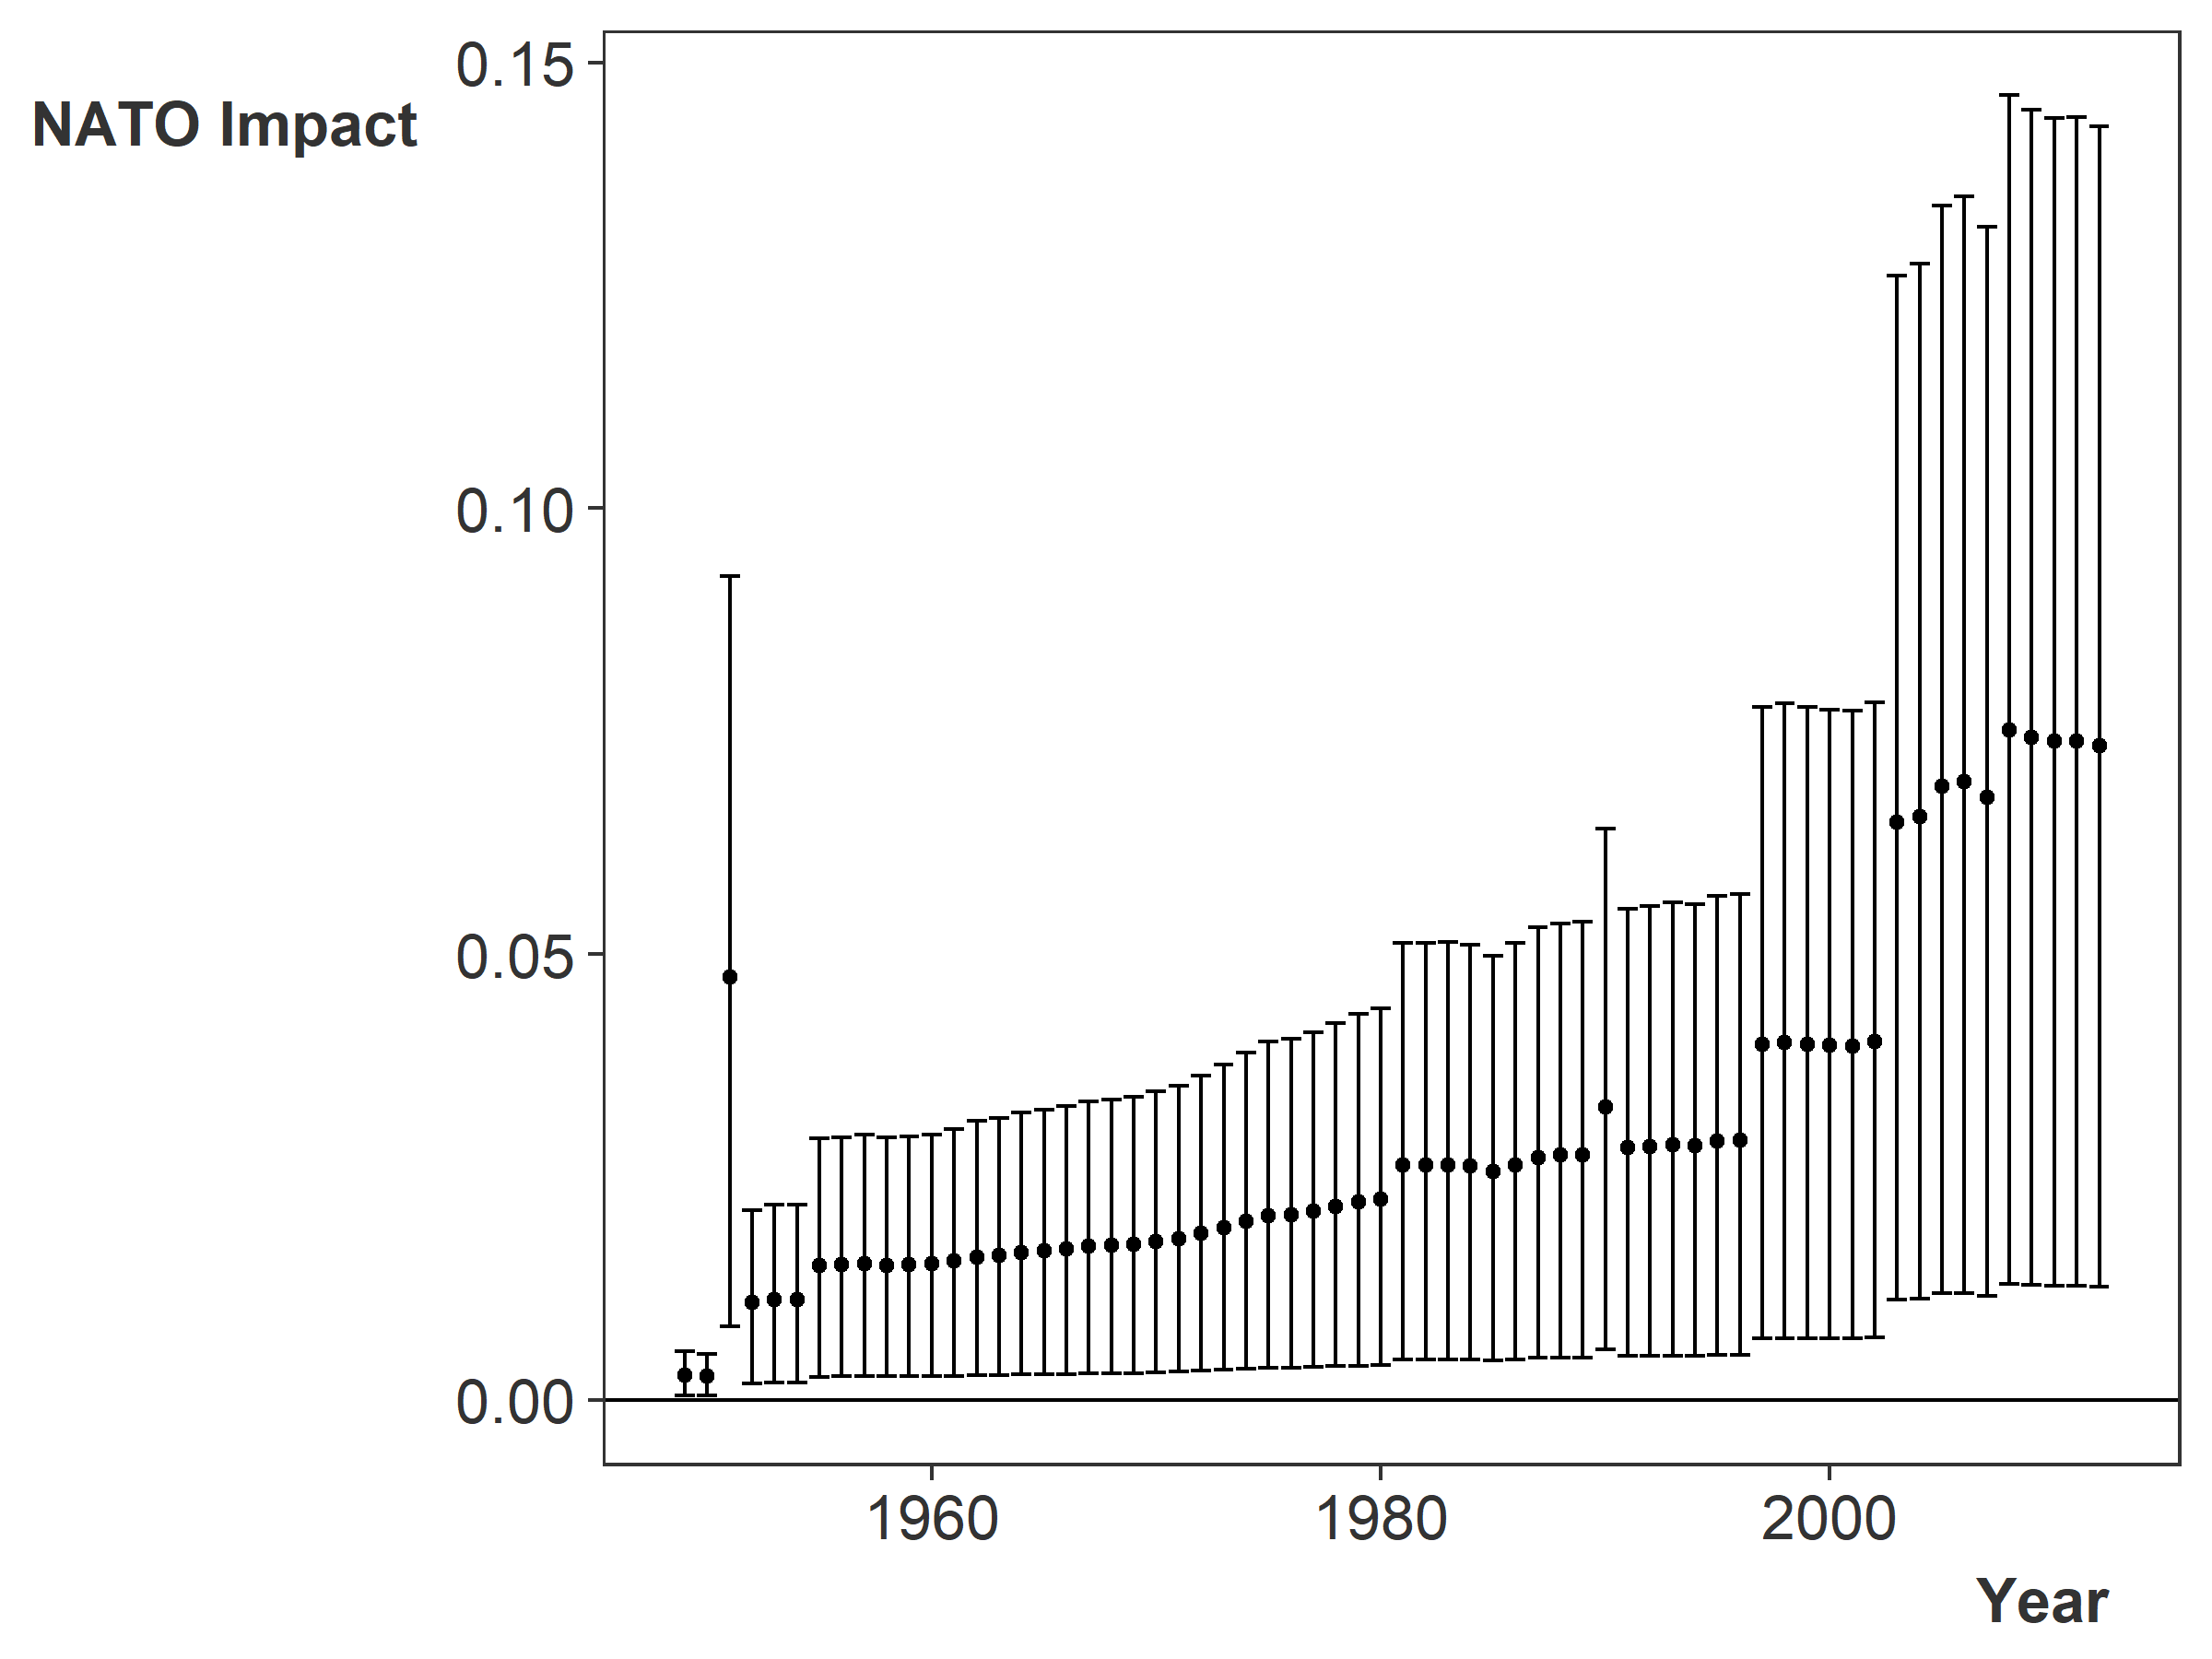
\includegraphics[width=0.95\textwidth]{nato-imp-us.png}
\end{figure}


\end{frame}

%------------------------------------------------


\begin{frame}{Correlates of War Spending Data}

Is messy... 

\begin{itemize}
\item Converted to standard units (British Pounds prior to 1914, US dollars thereafter). 
\item Occasionally smoothed with a seven-year moving average.
\item Interpolation with stable currency.
\end{itemize} 


\end{frame}


%------------------------------------------------

\begin{frame}{Alternative Measure of Military Spending}


\begin{itemize} 
\item Nordhaus et al 2012 data: mix of COW and SIPRI- fully rebased
\item 1949 to 2001
\item Same model: use changes in spending instead of percentage changes. 
\end{itemize}

\end{frame}


%------------------------------------------------

\begin{frame}{Alternative Measure of Military Spending: Results}

\begin{figure}[htbp]
	\centering
		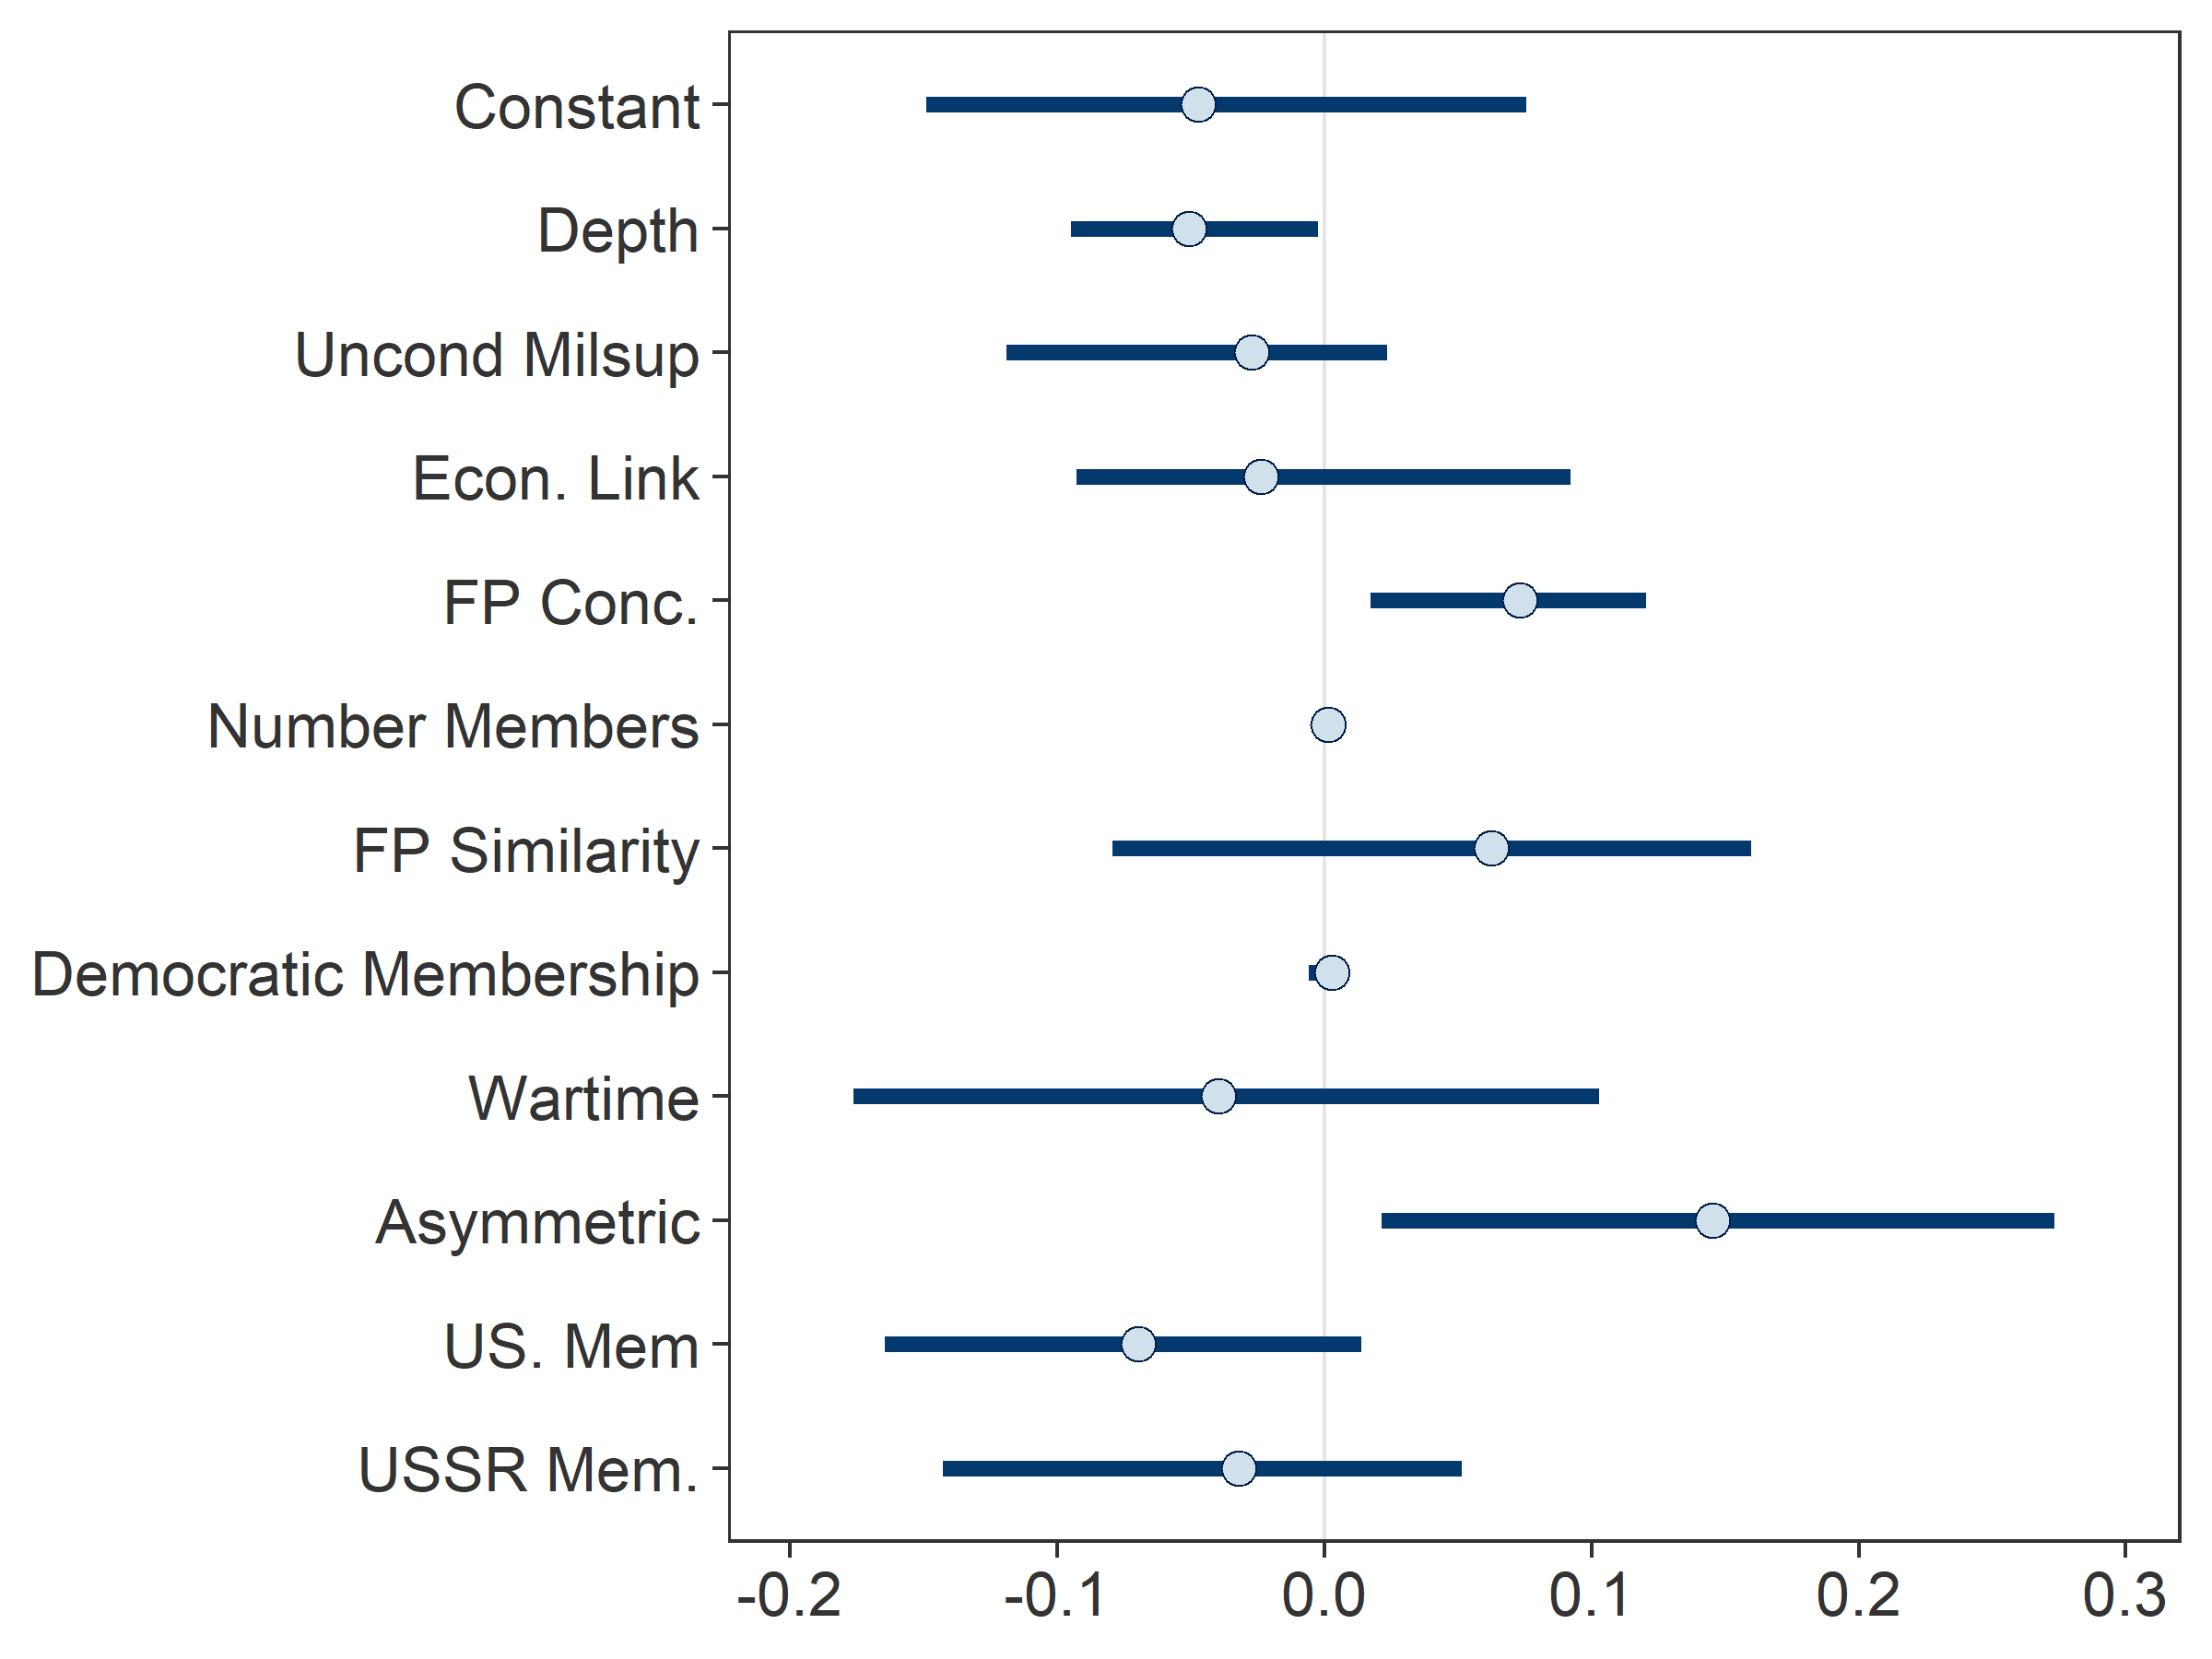
\includegraphics[width=0.85\textwidth]{beta-intervals-post45.png}
\end{figure}

\end{frame}

%------------------------------------------------


\begin{frame}{Single-Level Regression: Average Depth}


\begin{figure}[htbp]
	\centering
		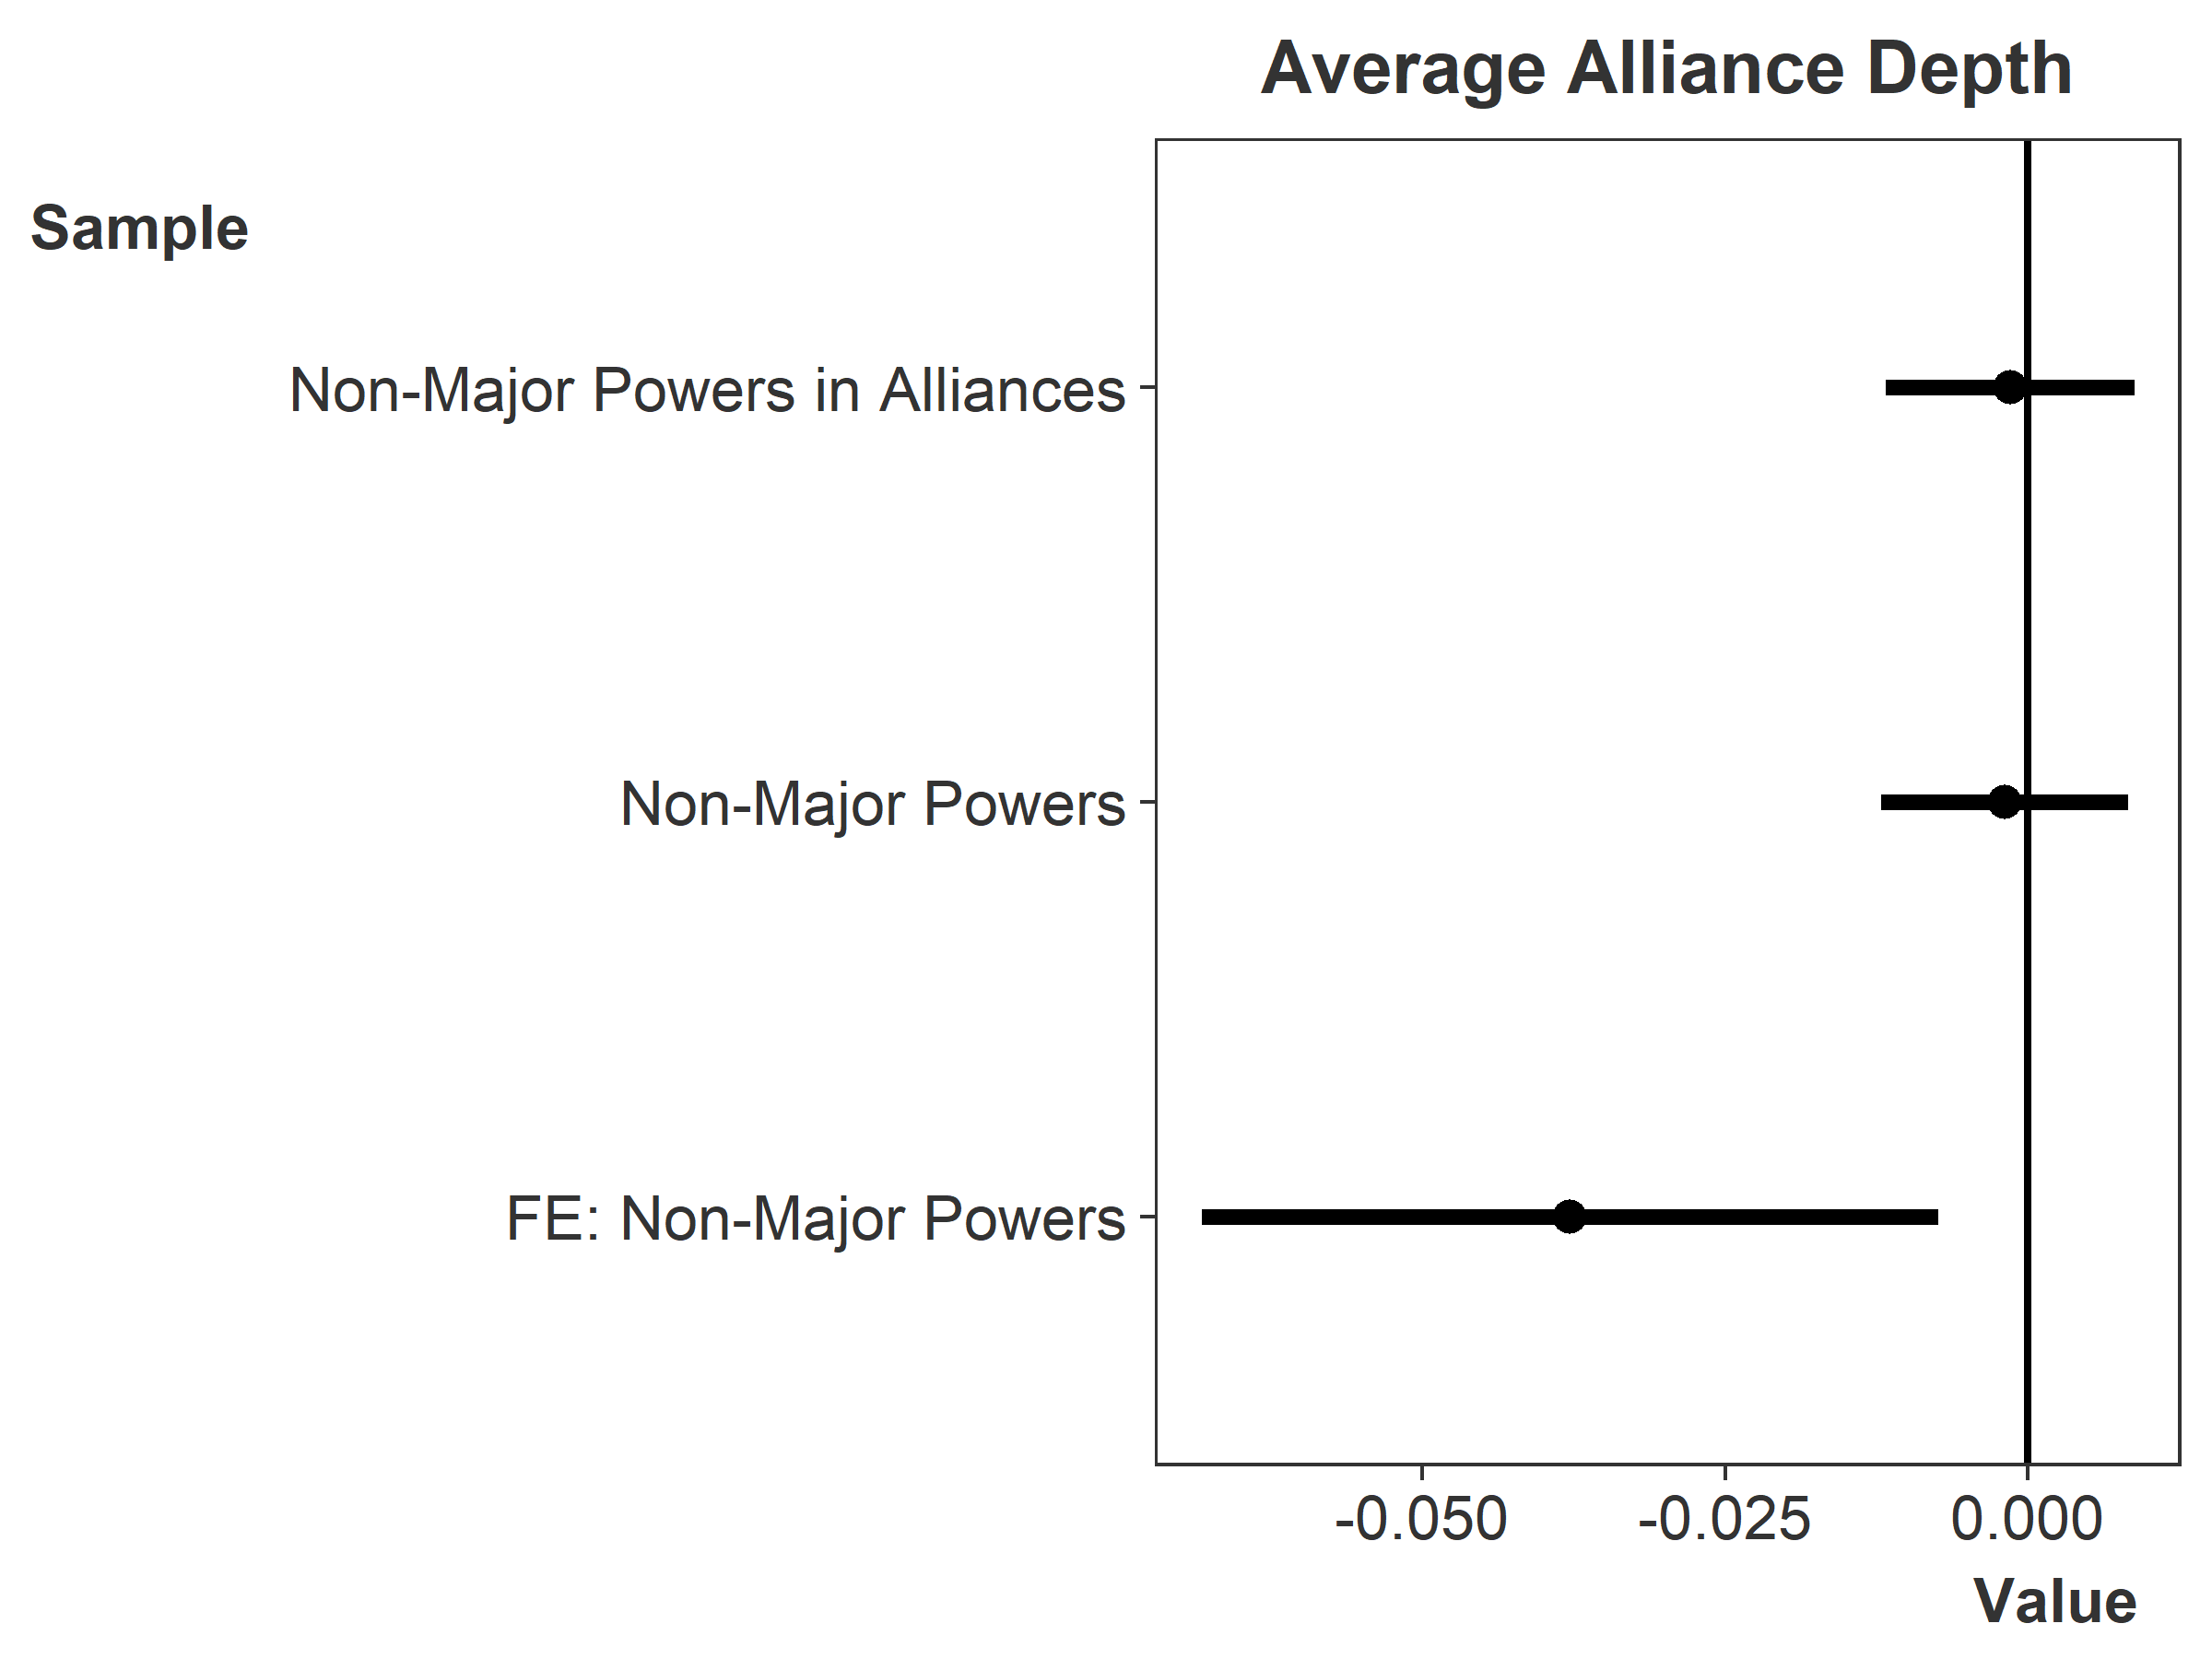
\includegraphics[width=0.95\textwidth]{single-level-average.png}
\end{figure}


\end{frame}

%------------------------------------------------

\begin{frame}{Single-Level Regression: Deep Alliance Dummy}


\begin{figure}[htbp]
	\centering
		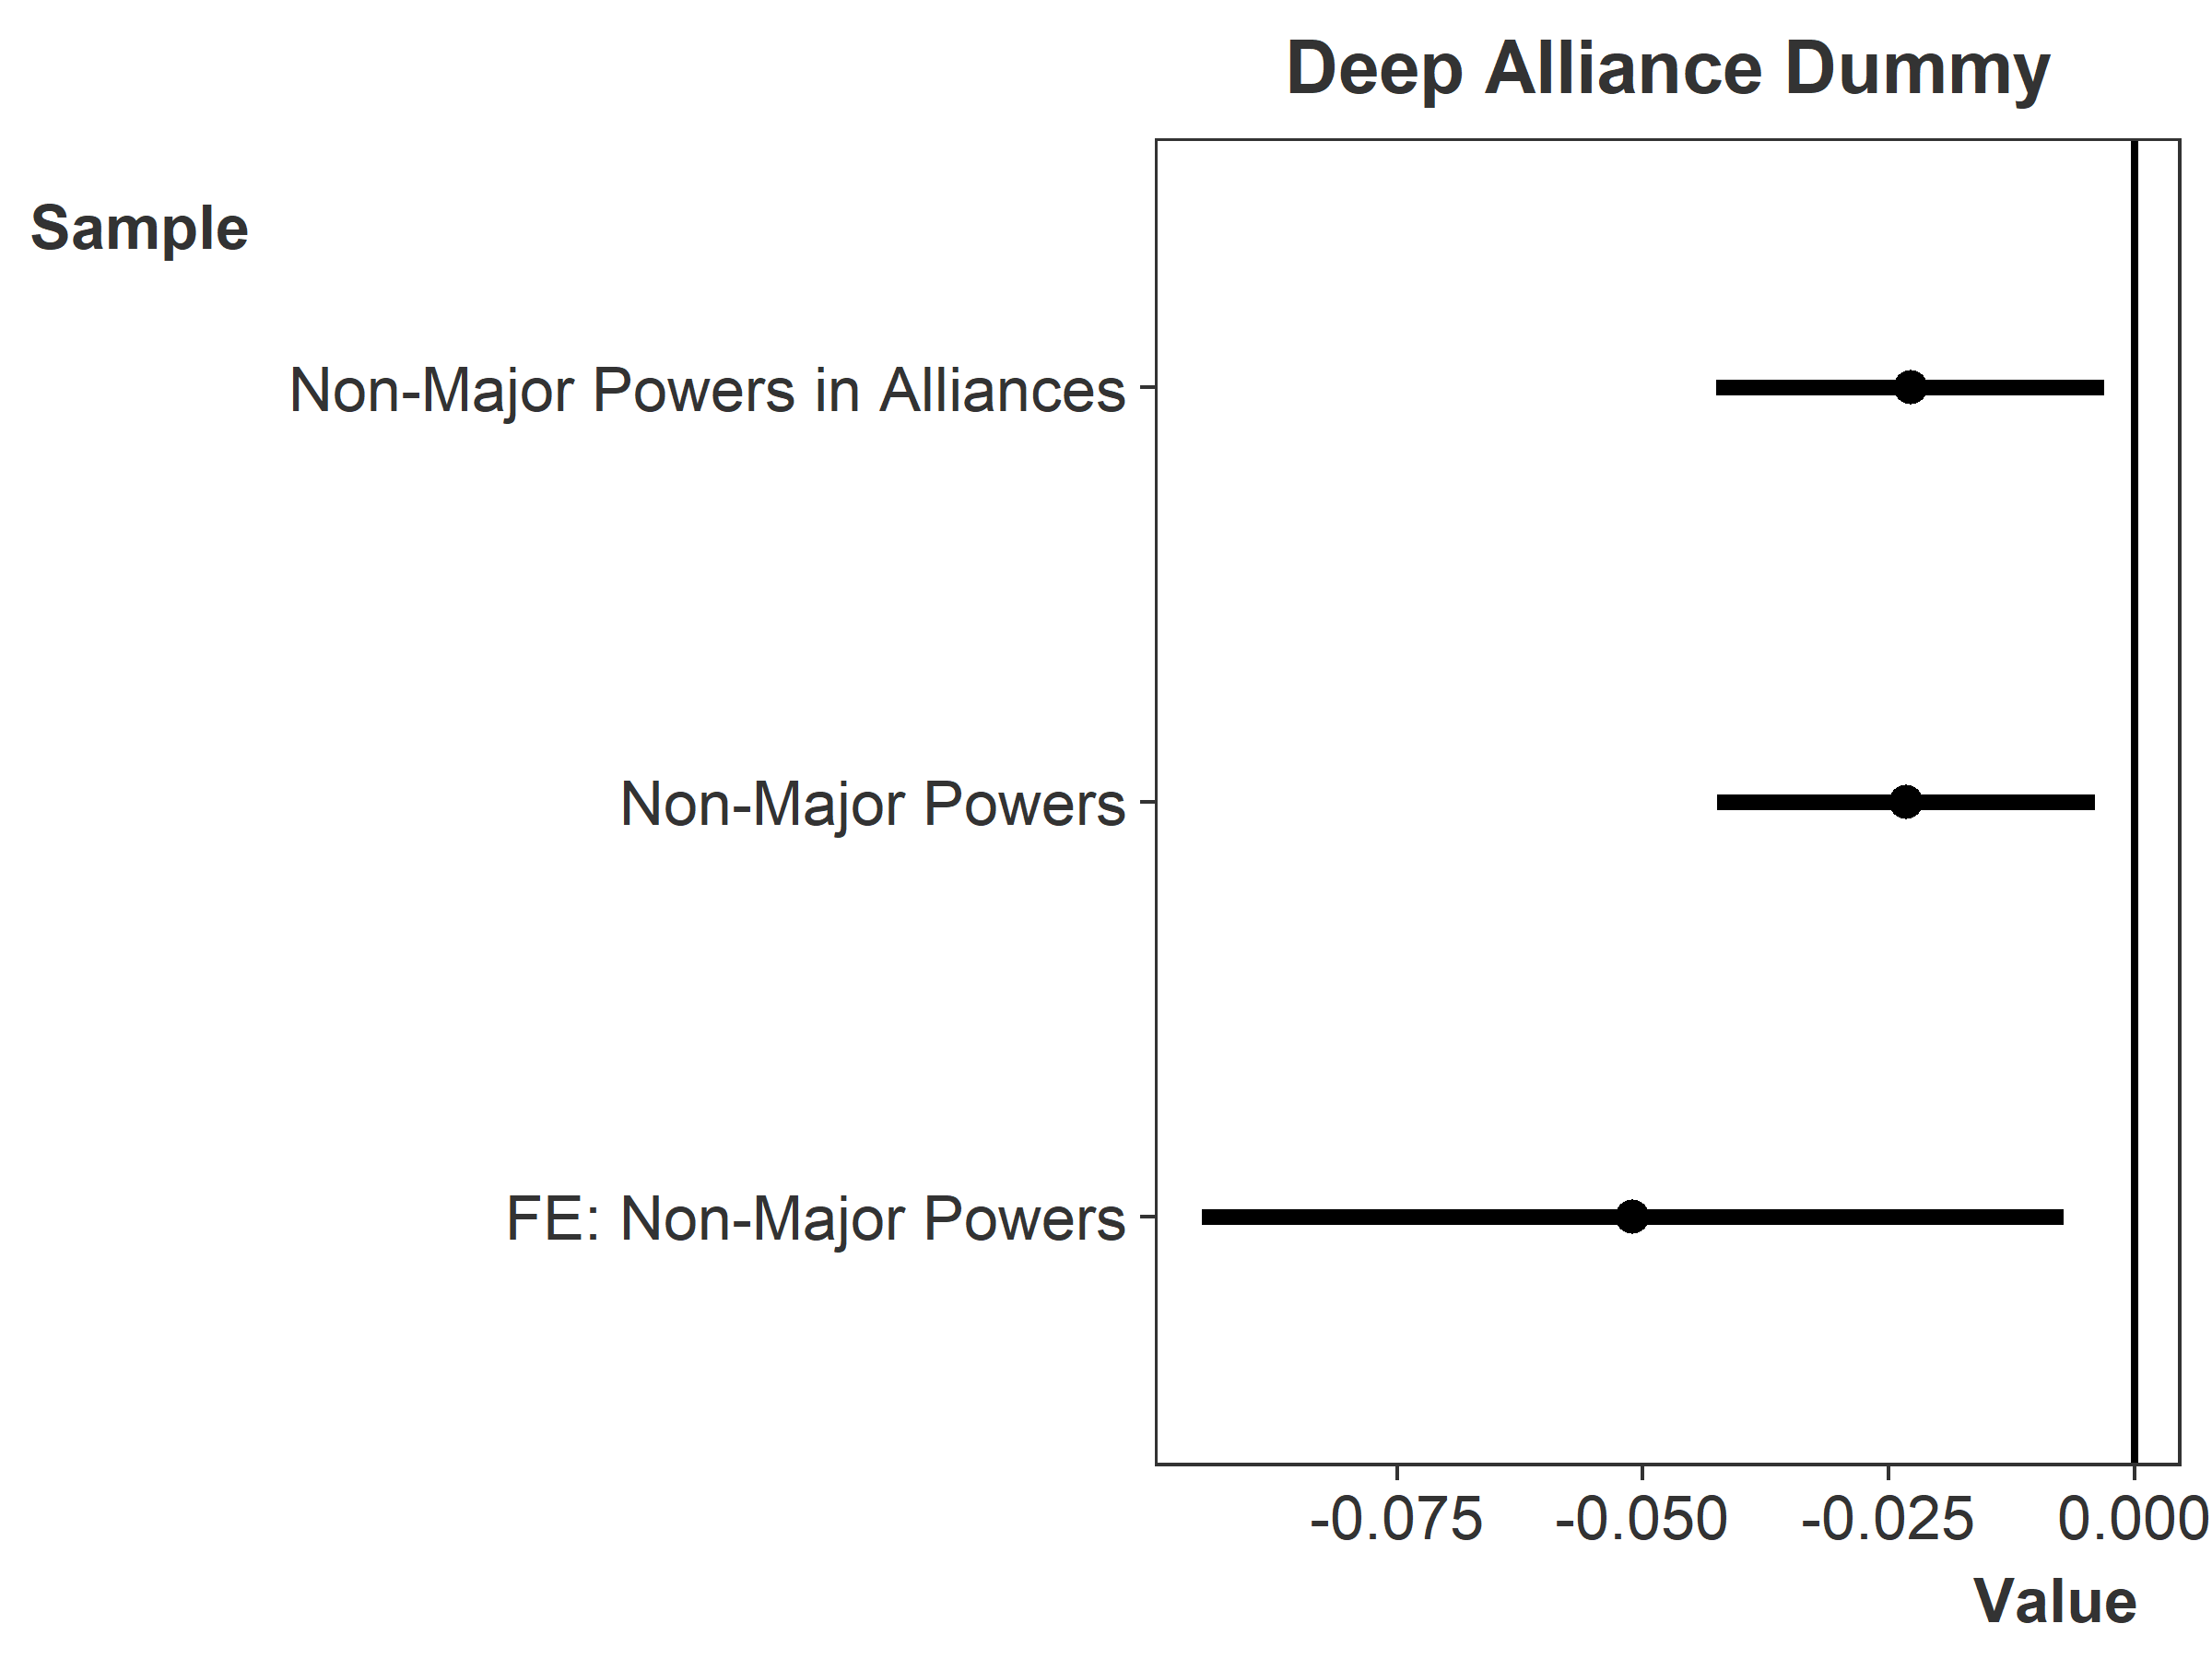
\includegraphics[width=0.95\textwidth]{single-level-dummy.png}
\end{figure}


\end{frame}



%------------------------------------------------


\begin{frame}{Bounds Analysis of Single-Level Regression}

\begin{figure}[htbp]
	\centering
		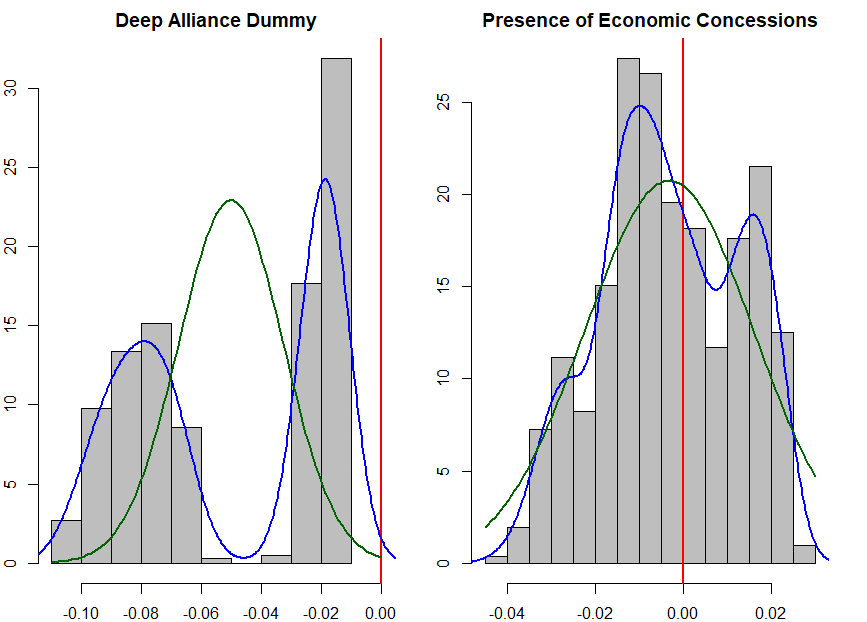
\includegraphics[width=0.95\textwidth]{eba-single-level.png}
\end{figure}


\end{frame}









%----------------------------------------------------------------------------------------

\end{document}
